%%%%%%%%%%%%%%%%%%%%%%%%%%%%%%%
% NB:
% This file requires 'biber' instead of 'bibtex' to create the bibliography. Please change the setting in your editor / makefile to call 'biber' instead of 'bibtex'.
%%%%%%%%%%%%%%%%%%%%%%%%%%%%%%%

% Determine general 'layout'
\documentclass[twoside, paper=a4, english, abstracton, 12pt, listof=entryprefix, toc=sectionentrywithdots, toc=listof]{scrartcl}

% Section title in serif font
\addtokomafont{disposition}{\rmfamily}

% duplicate Word-page borders
\usepackage[left=2.5cm,right=2.5cm, top=3cm, bottom=3cm]{geometry}

% languages
\usepackage[ngerman, english,main=english]{babel}

% 'draft' line is a switch: if there are huge figures, use draft to get a quick compile.
\usepackage[
%draft
]{graphicx}
\usepackage{caption}
\usepackage{subcaption}

% allows using German umlauts ä, ö, ü and ß
\usepackage[utf8]{inputenc}

% prevent 'out-of-Dimension' problems
\usepackage{etex}
\reserveinserts{30}

% Math-packages
\usepackage{amsmath}
\usepackage{amssymb}

% for reeeaally long tables
\usepackage{longtable}

% set links in the document; MUST BE LOADED prior to 'arydshln' and AFTER 'longtable', or else there will be lots of errors (see hyperref-manual)
\usepackage[unicode, hidelinks]{hyperref}
%\usepackage[unicode, colorlinks, allcolors=red]{hyperref}

\usepackage[toc, acronym, nogroupskip, nonumberlist]{glossaries}

\usepackage{listings}

% Table of contents more like in the Word-template
%\RedeclareSectionCommand[
%  tocindent=0pt,
%  tocnumwidth=2.3em,
%  tocbeforeskip=1em plus 1pt,
%  tocentryformat=\textbf,
%  tocpagenumberformat=\textbf
%]{section}

%\RedeclareSectionCommand[
%  tocindent=0.42cm,
%  tocnumwidth=1.8cm
%]{subsection}

%\RedeclareSectionCommand[
%  tocindent=0.42cm,
%  tocnumwidth=1.8cm
%]{subsubsection}

%\RedeclareSectionCommand[
%  tocindent=0.42cm,
%  tocnumwidth=1.8cm
%]{paragraph}

%Add linefeed after paragraph
\makeatletter
\renewcommand\paragraph{\@startsection{paragraph}{4}{\z@}%
  {-3.25ex\@plus -1ex \@minus -.2ex}%
  {1.5ex \@plus .2ex}%
  {\normalfont\normalsize\bfseries}}
\makeatother

%Add linefeed after subparagraph
\makeatletter
\renewcommand\subparagraph{\@startsection{subparagraph}{4}{\z@}%
  {-3.25ex\@plus -1ex \@minus -.2ex}%
  {1.5ex \@plus .2ex}%
  {\normalfont\normalsize\bfseries}}
\makeatother

\usepackage{changepage}   % for the adjustwidth environment
\newenvironment{identedParagraph}{\begin{adjustwidth}{2cm}{}}{\end{adjustwidth}}

% to have 'Figure' & 'Table' in front of the numbers in the listoffigures / -tables
\providecaptionname{english}{\listoflofentryname}{Figure}
\providecaptionname{ngerman}{\listoflofentryname}{Abb.}
\BeforeStartingTOC[lof]{\def\autodot{:}}

\providecaptionname{english}{\listoflotentryname}{Table}
\providecaptionname{ngerman}{\listoflotentryname}{Table}  % Yes, english here as well... TeX is still in german-mode when creating LoT
\BeforeStartingTOC[lot]{\def\autodot{:}}

%Rename how the Code should be named
%\renewcommand\lstlistingname{Code}
%rename how the List should be named
\renewcommand{\lstlistlistingname}{List of \lstlistingname s}

\usepackage[table]{xcolor}

\definecolor{mygreen}{rgb}{0,0.6,0}
\definecolor{mygray}{rgb}{0.5,0.5,0.5}
\definecolor{mymauve}{rgb}{0.58,0,0.82}
\definecolor{ultramarine}{rgb}{0,0.125,0.376}
\definecolor{backcolour}{rgb}{0.95,0.95,0.92}

\lstset{
    basicstyle=\ttfamily\footnotesize\color{ultramarine},
    breaklines=true,
    captionpos=b,
    commentstyle=\color{mygreen},
    keywordstyle=\color{blue},
    stringstyle=\color{mymauve},
    showstringspaces=false,
    numbers=left,                    
    numbersep=5pt,
    backgroundcolor=\color{backcolour},
}

\lstdefinelanguage{CXX}[]{C++} {
    basicstyle=\ttfamily\footnotesize,
    morekeywords={constexpr,static_assert,override,is_base_of_v,is_base_of_template_v,conditional_t,ifdef,endif},
    breaklines=true,
    captionpos=b,
    commentstyle=\color{mygreen},
    keywordstyle=\color{blue},
    emphstyle=\color{ultramarine},
    stringstyle=\color{mymauve},
    showstringspaces=false,
    frame=tb,
    aboveskip=20pt,
}

\lstdefinelanguage{SCXML}[]{XML} {
    basicstyle=\footnotesize,
    morekeywords={scxml,state,transition,invoke,initial},
    breaklines=true,
    captionpos=b,
    commentstyle=\color{mygreen},
    keywordstyle=\color{blue},
    emphstyle=\color{ultramarine},
    stringstyle=\color{mymauve},
    showstringspaces=false,
    frame=tb,
    aboveskip=20pt,
}


% Ploting
\usepackage{bubbleplot}
\usepackage{tikz-uml}

\definecolor{1992}{rgb}{1, 0.5, 0.5}
\definecolor{1995}{rgb}{1, 0.6363636363636364, 0.5}
\definecolor{2001}{rgb}{1, 0.7727272727272727, 0.5}
\definecolor{2002}{rgb}{1, 0.9090909090909091, 0.5}
\definecolor{2003}{rgb}{0.9545454545454546, 1, 0.5}
\definecolor{2006}{rgb}{0.8181818181818182, 1, 0.5}
\definecolor{2007}{rgb}{0.6818181818181819, 1, 0.5}
\definecolor{2008}{rgb}{0.5454545454545454, 1, 0.5}
\definecolor{2010}{rgb}{0.5, 1, 0.5909090909090908}
\definecolor{2011}{rgb}{0.5, 1, 0.7272727272727273}
\definecolor{2012}{rgb}{0.5, 1, 0.8636363636363635}
\definecolor{2013}{rgb}{0.5, 1.0, 1}
\definecolor{2014}{rgb}{0.5, 0.8636363636363638, 1}
\definecolor{2015}{rgb}{0.5, 0.7272727272727271, 1}
\definecolor{2016}{rgb}{0.5, 0.5909090909090908, 1}
\definecolor{2017}{rgb}{0.5454545454545454, 0.5, 1}
\definecolor{2018}{rgb}{0.6818181818181817, 0.5, 1}
\definecolor{2019}{rgb}{0.8181818181818183, 0.5, 1}
\definecolor{2020}{rgb}{0.9545454545454546, 0.5, 1}
\definecolor{2021}{rgb}{1, 0.5, 0.9090909090909092}
\definecolor{2022}{rgb}{1, 0.5, 0.7727272727272729}
\definecolor{2023}{rgb}{1, 0.5, 0.6363636363636362}

\pgfplotsset{
  colormap={yearcolor}{
    color=(1992),
    color=(1995),
    color=(2001),
    color=(2002),
    color=(2003),
    color=(2006),
    color=(2007),
    color=(2008),
    color=(2010),
    color=(2011),
    color=(2012),
    color=(2013),
    color=(2014),
    color=(2015),
    color=(2016),
    color=(2017),
    color=(2018),
    color=(2019),
    color=(2020),
    color=(2021),
    color=(2022),
    color=(2023),
  }
}

%does what it says on the lid
\usepackage{multirow}

%for texttimes, trademark (\texttrademark)
\usepackage{textcomp}

% turns on latin modern fonts, e.g. italics in headlines
\usepackage{lmodern}

% page numbers and header
\usepackage[automark,headsepline]{scrlayer-scrpage}
\setkomafont{pagehead}{\normalfont}

%better tables
\usepackage{tabularx}

\newcolumntype{s}{>{\columncolor{teal!30}} c}
\newcolumntype{t}{>{\columncolor{teal!10}} c}

% place figures HERE and nowhere else! Option: [H]
\usepackage{float}

\usepackage{comment}
% at least for \begin{comment}...\end{comment} <- comment out sections
\usepackage{verbatim}

% for captions
\usepackage[format=plain,labelfont={it,small},font={it,small}]{caption}

% have dashed separators in tables ':'
\usepackage{arydshln}

% needed by excel2latex for 'addlinespace'
\usepackage{booktabs}

%line skip 1.5
\usepackage[onehalfspacing]{setspace}

% varying space character after 'newcommand' constructs; if normal space, then space, if comma or dot, then no space
\usepackage{xspace}

% References list - because it schould be APA-style as in Word
%\usepackage[style=apa,backend=biber]{biblatex}
\usepackage[
        style=ieee,
        backend=biber
    ]{biblatex}

\addbibresource{biblio.bib}

% biblatex would like to have this package loaded
\usepackage{csquotes}

% counters count into depth 4 for TOC; depth 4 is paragraph
%\usepackage{titlesec}
\setcounter{secnumdepth}{3}
\setcounter{tocdepth}{2}


% Distances between paragraphs
\setlength{\parskip}{0.5em}
\setlength{\parindent}{0ex}
%\setlength{\parindent}{1em}

% Page numbers, header, footer
\pagestyle{scrheadings}

% Header a bit larger
\setlength{\headheight}{1.1\baselineskip}

\clearpairofpagestyles
\ihead{\headmark}
\ohead{\pagemark}

% remove number in front of section name (in header)
\renewcommand*{\sectionmarkformat}{}

% uncomment to supress printing images
%\renewcommand{\includegraphics}[2][]{\fbox{}}
\DeclareUnicodeCharacter{0301}{*************************************}
\makenoidxglossaries

%----Abbreviations-----
%
\newglossaryentry{ontology} {
        name=ontology,
        description={Is a mark up language specially suited for scientific documents}
}
%----Acronyms-----
%
\newcommand{\acronym}[2]{\newacronym{#1}{#1}{#2}}

\acronym{IEEE}{Institute of Electrical and Electronics Engineers}
\acronym{ISO}{International Organisation for Standardisation}
\acronym{SPLE}{Software Product Line Engineering}

\newacronym{sms}{SMS}{Systematic Mapping Study}
\newacronym{ep}{EP}{Entwicklung Plattform}
\newacronym{cae}{CAE}{Computer Aided Engineering}
\newacronym{cad}{CAD}{Computer Aided Design}


\newacronym{uri}{URI}{Uniform Resource Identifier}
\newacronym{url}{URL}{Uniform Resource Locator}
\newacronym{urn}{URN}{Uniform Resource Name}
\newacronym{iri}{IRI}{Internationalized Resource Identifier}
\newacronym{rdf}{RDF}{Resource Description Framework}
\newacronym{rdfs}{RDFS}{Resource Description Framework Schema}
\newacronym{sparql}{SPARQL}{SPARQL Protocol and RDF Query Language}
\newacronym{ai}{AI}{Artificial Intelligence}
\newacronym{ascii}{ASCII}{American Standard Code for Information Interchange}
\newacronym{http}{HTTP}{Hypertext Transfer Protocol}
\newacronym{lov}{LOV}{Linked Open Vocabularies}
\newacronym{owl}{OWL}{Web Ontology Language}
\newacronym{swrl}{SWRL}{Semantic Web Rule Language}
\newacronym{sql}{SQL}{Structured query language}


\newacronym{fol}{FOL}{First Order Logic}

\newacronym{ui}{UI}{User Interface}

\newacronym{tdb2}{TDB2}{Triplet Data Base}

\newacronym{cbr}{CBR}{Case Based Reasoning}

\newacronym{json}{JSON}{JavaScript Object Notation}

\newacronym{xml}{XML}{Extensible Markup Language}

\newacronym{psm}{PSM}{Problem-Solving Methods}


\begin{document}

\pagenumbering{gobble}

\begin{titlepage}

    \begin{center}

        \begin{figure}
            \centering
            
\includegraphics[width=0.35\textwidth]{images/RPTU-Logo.png}
        \end{figure}
        
        \textbf{Rheinland-Pfälzische Technische Universität Kaiserslautern-Landau}\\[2\baselineskip]

        Master's Thesis

        \vspace{0.8cm}

        \Huge
        \textbf{Feasibility Study on Usage of Semantic Technology to Support Configuration Processes in Systems Engineering}
        \vspace{1.5cm}

        \normalsize
        submitted by

        \large
        \textbf{Dannick Arnold Kwengang Tankeu}

        %\vfill

        \vspace{1.5cm}

        \normalsize
        in cooperation with the

        \vspace{0.8cm}

        \textbf{Fraunhofer Institute for Experimental Software Engineering}

        \vspace{1.0cm}

        
\includegraphics[width=0.35\textwidth]{images/logo_iese}

        \vspace{1.0cm}

        \large
        \begin{tabular}{l l l}
            \textbf{First Advisor}  &: & \textbf{Prof.~Dr.-Ing.~Peter Liggesmeyer} \\
            \textbf{Second Advisor} &: & \textbf{M. Sc.~Christian Malek} \\
        \end{tabular}

    \end{center}
\end{titlepage}

\clearpage

\begin{otherlanguage}{ngerman}
%
%Please leave the text below in German!!!
%
\phantomsection
\addsec*{Declaration}
%
I assure you that I have written the Master's thesis independently and have only used the sources
and resources indicated and that I have identified the passages taken literally or in terms of
content from the sources used.\\[2ex]
\makebox[5cm][l]{Place, date}\hfill\makebox[4cm][l]{Signature}\\[1cm]
\makebox[5cm]{\hrulefill}\hfill\makebox[4cm]{\hrulefill}

\end{otherlanguage}

\clearpage

\addsec*{Abstract}

Text

KEYWORDS: Software Product Line Engineering (SPLE).


\clearpage

\addsec*{Acknowledgements}

Since I started working on this thesis, I've been able to broaden my horizons and acquire extraordinary knowledge. It has been possible for me to work night and day on this thesis while maintaining a high level of dynamism, thanks to my enthusiasm for semantic technologies and intelligent systems. I have done my best to provide work that can be used in future research, as well as to provide a reliable, resilient and usable solution.\\
On this occasion, I would like to thank Christian Malek, who not only helped me greatly in understanding the specifics of my subject, but also took the time to accompany me in the implementation and writing of this paper. I would also like to thank Dr. Martin Becker and Jana Heinrich, who were a great help during our numerous meetings and workshops. Finally, I would like to thank Prof. Dr. Peter Liggesmeyer for supervising my thesis.


\clearpage

\pagenumbering{Roman}

{
\hypersetup{hidelinks}

\phantomsection
\addcontentsline{toc}{section}{Table of Contents}
\renewcommand{\contentsname}{Table of Contents}
\tableofcontents
\clearpage

\phantomsection
\setglossarystyle{long}
\setlength\LTleft{0pt}
\setlength\LTright{0pt}
\setlength\glsdescwidth{0.8\hsize}
\printnoidxglossary[title=List of Abbreviations, type=\acronymtype]
\clearpage

\phantomsection
\listoftables
\clearpage

\phantomsection
\listoffigures
\clearpage
\phantomsection
\begingroup
\let\oldnumberline\numberline
\renewcommand{\numberline}[1]{Listing \oldnumberline{#1}}
\lstlistoflistings
\endgroup
\cleardoublepage

}

\setcounter{table}{0}

\pagenumbering{arabic}

\section{Introduction\label{sec:introduction}}


\subsection{Motivation}
In engineering, it is extremely important to set up simulations during the design phase (left-hand side of the V-Model) \cite{hammami2015thefose}. This enables the behavior of the product or components to be predicted at a very early stage, so that potential problems can be anticipated.  As technology advances, the automotive sector relies more and more on simulations to drive innovation and efficiency \cite{hammami2015thefose}. However, with the increasing complexity of systems, the configuration of these simulations poses significant challenges. The process of configuring a simulation depends on a number of factors, properties and the objective being pursued. Depending on the values of these factors, a basic simulation can be obtained. Because of their large number and the interdependence between them, it quickly becomes complicated to know which values to choose and what the repercussions of this choice will be \cite{hammami2015thefose, horsch2021osmo, spelten2023simulation}. This problem becomes even more obvious when the engineer responsible for the configuration lacks experience. It therefore becomes necessary to set up a tool to assist in the implementation of simulations. As part of the \textbf{\acrfull{ep} 4.0 project}, a platform is being developed to help simulation engineers select previous load cases and determine parameter values for new simulations. This will make it possible to benefit from the experience accumulated in previous projects over time.


\subsection{Research Goals}
To be able to exploit these old simulations, their metadata must be stored efficiently and robustly. Semantic technologies, in particular ontologies, offer a viable solution for structuring, modelling and storing this data \cite{horsch2021osmo, spelten2023simulation}. These technologies use formal semantics to give meaning to raw data, thereby making it machine-readable. This thesis undertakes an in-depth study of the feasibility of using semantic technologies to improve configuration processes in systems engineering.\\

From this, the main objective can be broken down into several high-level objectives:

\begin{itemize}
  \item \textbf{G1\label{G1}}: The first objective is to create an ontology that can be used to represent simulations, their meta-information, and all the interdependencies and rules that apply to them.

    \item \textbf{G2\label{G2}}: The second objective is to create an automated framework for identifying similar simulations from previous project databases, as well as a mechanism for suggesting viable parameter values throughout the process.
    
    \item \textbf{G3\label{G3}}: Another objective of this thesis is to develop a prototype web application, which consumes the services of our framework. This application should allow a user to configure a basic simulation step by step using the data and rules defined in our ontology.

\end{itemize}


\subsection{Research Questions\label{subsec:reseques}}

In order to determine whether the use of semantic technologies actually brings benefits in supporting process configuration in systems engineering, the following research questions have been defined: 

\begin{itemize}
    \item \textbf{Q1\label{Q1}}: What are the main challenges and limitations of current configuration processes for simulations in the automotive industry?
    \item \textbf{Q2\label{Q2}}: How can semantic technology be used to support simulation configuration processes?
    \item \textbf{Q3\label{Q3}}: What are the requirements of a semantic-based configuration tool for automotive simulations?
    \item \textbf{Q4\label{Q4}}: What are the existing semantic technologies and standards applicable to the field of systems engineering and simulation configuration, and how can they be adapted to support simulation configuration processes?
 \end{itemize}


\clearpage
\subsection{Research Approach}
The research approach used consists firstly of understanding the different areas involved. This enables the identification of the main limitations and challenges inherent in current simulation configuration processes in the automotive industry. It critically assesses the shortcomings that hinder the seamless integration and adaptation of new simulation configurations.
In order to have a structured and well-documented research process, the Thematic Mapping study method was chosen.\\

This defined the essential requirements for a semantic-based configuration tool tailored to the specific needs of simulation configuration. Focusing on the critical features and functionalities that such a tool must encompass.\\

The research also includes an in-depth analysis of existing semantic technologies and standards applicable to the field of systems engineering and simulation configuration. By assessing their adaptability and relevance to the domain, the study provides insight into the potential changes and extensions needed to adapt these technologies to the unique requirements of simulation configuration.\\

The approach described can be summarized in the following steps, which can also be repeated iteratively:

\begin{enumerate}
    \item \textbf{Find a Problem.} Find an interesting and practically relevant problem that also
        has the potential for theoretical contribution.
    \item \textbf{Understand.} Establish a baseline and obtain a practical and theoretical
        understanding of both the concrete problem and the topic area. This includes the
        elicitation of the state of practice via, e.g.,~interviews or observations and a
        literature review to get an overall picture of the relevant body of knowledge.
    \item \textbf{Set goals.} Define quantifiable goals that can later be used to validate the
        solution.
    \item \textbf{Innovate.} Use the obtained knowledge to construct an innovative solution
        concept and implement a proof of concept solution.
    \item \textbf{Analyze.} Analyze the solution and demonstrate that it works. Examine the scope
        of applicability and generalize. Reason how the solution can be applied to other problem
        domains or organizations. Show theoretical contributions and novelty.
\end{enumerate}


\subsection{Key Contributions}
Overall, this thesis contributes to a global understanding of the practical applications of semantic technologies in the field of systems engineering. It proposes the development of a knowledge model (ontology) for simulations. The ontology developed will provide a better understanding of the structure of a simulation and a formal vocabulary. This formalism is of paramount importance, in particular to enable global understanding and the use of the same terms by all users.\\

The framework we have developed makes it possible to identify the old simulations that are most similar to the simulation currently being configured, and proposes the (most plausible) values that a parameter could have at each stage throughout the configuration process. These two services depend heavily on the information already entered in the previous stages of the cases stored in the database.


\subsection{Thesis Structure}
This thesis report begins with an overview of the foundations of systems engineering simulations in \textbf{Chapter \ref{sec:foundation}}, where we analyze the steps in the configuration process and the metadata that is important to us. This understanding will be of paramount importance when structuring our knowledge graph (Ontology). Next, the concept of an “Expert System” will be explored, enabling us to understand how such tools can assist engineers. This chapter also includes a study of the various semantic technologies such as RDF, OWL, SPARQL, etc., together with examples of their use and applications. \\

In order to analyze previous research work more effectively in the context of the theme of this thesis, a “Systematic mapping study” will be carried out in \textbf{Chapter \ref{sec:relwork}}. Then, depending on the analysis made, a result on the state of current studies will be elaborate.\\

\textbf{Chapter \ref{sec:conception}} deals with the modelling of simulations using ontologies. Concepts, properties, important entities and the relationships between them are identified. This information will be used to create the ontology in \textbf{Chapter \ref{sec:implementation}}. In this chapter, the operating mode and algorithms (pseudocode) of “Case-Based Reasoning” and “Rule-Based Reasoning” will be studied. \\

In addition to setting up the ontology, the reasoning mechanisms analyzed in \textbf{Chapter \ref{sec:conception}} will be implemented in \textbf{Chapter \ref{sec:implementation}}. A web application (prototype) will also be set up as a demonstration tool. It will be used for the evaluation tests in \textbf{Chapter \ref{sec:evaluation}}.\\

\textbf{Chapter \ref{sec:evaluation}} is devoted solely to evaluating the solution developed. Various use cases will be defined and then executed. Based on the results, an analysis will be made to determine whether the proposed solution effectively addresses the problems identified. This chapter extends the discussion to the benefits obtained from the developed solution, as well as the limitations that can still be identified.\\

Finally, in \textbf{Chapter \ref{sec:conclusion}} the conclusion will be presented. It is accompanied by suggestions for future work.


\clearpage
\section{Foundation\label{sec:foundation}}
In this chapter, the basic concepts fundamental to understanding the subject of the thesis will be explained. This will allow a better understanding of the following chapters and the proposed solutions. Firstly, the foundations of systems engineering will be presented. Then the notions of \acrshort{cad}, \acrshort{cae}, and “Expert System” will be explained. This will be followed by an introduction to semantic technologies. This will be followed by an analysis of the use of semantic technologies in the field of systems engineering. 

\subsection{System Engineering \label{sec:sysen}}
Systems engineering is a multidisciplinary approach to the design, implementation and management of complex systems throughout their life cycle (see Figure). It embraces a holistic perspective that takes into account the interactions and interdependencies between different components in order to achieve optimal performance and functionality. Systems engineering deals with work processes, optimisation methods and risk management tools in projects. Systems engineering ensures that all likely aspects of a project or system are considered and integrated as a whole. In the context of the automotive industry, where complex systems and simulations play a central role, the application of systems engineering principles becomes paramount.

\subsubsection{Core Concepts}
    The key principles of systems engineering are as follows:
    \begin{itemize}
      \item Requirements engineering: this phase consists of determining and documenting the needs and constraints that the system must satisfy. In the context of simulation configuration, understanding requirements is crucial to accurately model and simulate real-world automotive scenarios.
      
      \item System design: this phase involves transforming the requirements into a system plan. It involves assigning functions to components, taking into account factors such as efficiency, reliability, and maintainability. For simulation configuration, this step is essential to create a framework that aligns with the specific attributes of automotive simulations.
      
      \item Integration and testing: Systems engineering emphasizes the importance of rigorous testing and integration to ensure that all components work perfectly together. This is particularly relevant in the context of simulation configuration, where the accuracy and reliability of results depend on the effective integration of different simulation parameters.
      
      \item Lifecycle management: Systems engineering goes beyond the initial design and implementation phases. It involves continuous monitoring, maintenance and adaptation to changing requirements throughout the system's lifecycle. This perspective is crucial to the longevity and adaptability of simulation configurations in the dynamic automotive landscape.

    \end{itemize}

    
\subsubsection{V-Model}
The V-model illustrates systems development by highlighting the verification and validation stages. A graphical representation of this model is shown in Figure \ref{fig:v-model}. The system specification and detailed software design are presented on the left-hand side of the “V”, along with the steps leading to implementation. The steps mentioned on the left-hand side must be verified and validated on the right-hand side of the “V”. It also includes the integration of systems and software. Each step on the left is directly linked to a test step. Once the first stage has been successfully completed, the next stage begins.\\

\begin{figure}[H]
    \centering
    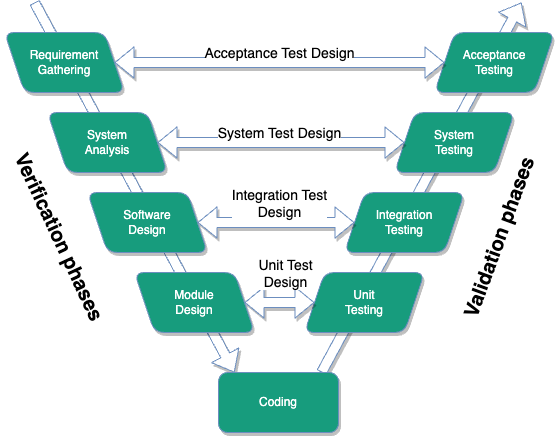
\includegraphics[scale=0.6]{images/V-Model.png}
    \caption{\label{fig:v-model} V-Model }
\end{figure}

With the evolution of technology, many software applications exist to cover these different stages more effectively. 

\subsection{\acrlong{cae} and Simulation}
\acrfull{cae}, also known as digital engineering or computer-aided engineering, brings together all the digital and software resources usually used by engineers to design, simulate and validate new products and industrial processes using sophisticated algorithms. \acrshort{cae} tools enable the physical properties of a product to be tested and simulated, so that it can be optimized on the basis of the results of a numerical analysis.

    \subsubsection{Simulation-driven design}
    Typically, \acrshort{cae} involves pre-processing, solving and post-processing stages \cite{karlberg2013state}. During the pre-processing phase, engineers model the system, the physical properties of the design, and the operational environment in the form of applied constraints or loads. In order to correctly configure the resulting simulations, it is crucial that this modelling incorporates all parts of the environment to which the product will be exposed (including forces, temperatures, etc.).  The quality of the simulation is largely determined by the accuracy of the conditions to which the product will be exposed. The model is then solved using simulations before the results are presented for review during post-processing. \\

    Whereas physical prototyping takes days or even weeks, simulations take just a few hours at most. Although physical prototyping is unavoidable, simulations can help reduce the number of prototypes needed before production \cite{sellgren1999simulation}.\\
    
    Figure\ref{fig:v-model-sim} shows the different types of simulations and tests throughout the “V” model presented above. Initial design and simulation of \acrfull{cad} geometry under appropriate conditions is the \acrshort{cae}'s standard workflow. Based on the results of the simulation, the design is improved. This process may need to be repeated until the product requirements are met and virtually confirmed. If there are differences in behavior between the digital prototype and expectations, the \acrshort{cad} model or input data can be adjusted \cite{sellgren1999simulation, jeon2016automatic}. This process speeds up product development because there is no need to create physical prototypes in the early stages of development.

    \begin{figure}[h]
        \centering
        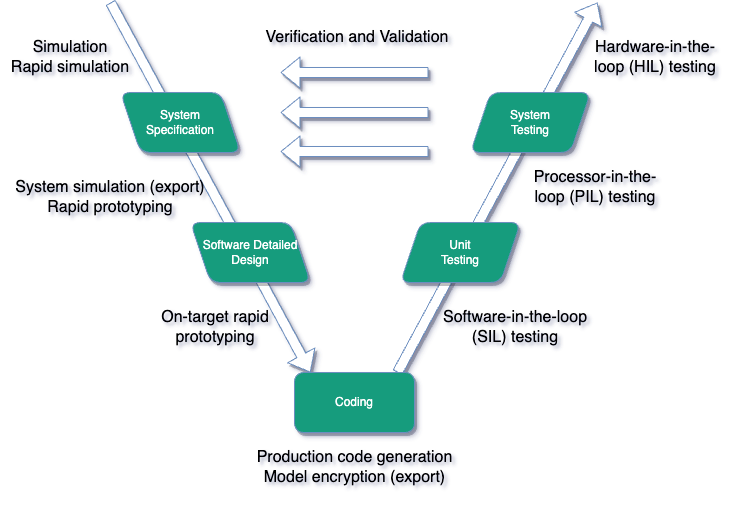
\includegraphics[scale=0.6]{images/Foundation-V-Model-Sim.drawio.png}
        \caption{\label{fig:v-model-sim} V-Model with simulations \cite{validVerifSys} }
    \end{figure}


    \subsubsection{Advantages}
    One of the main advantages of this approach is that it only takes a few hours, whereas it takes several days or even weeks to build and test physical prototypes. Of course, there will always be a need to build a physical prototype at some point, but \acrshort{cad} greatly reduces the number of prototypes required. The use of \acrshort{cad} and the resulting reduction in the need for physical prototypes means that product development costs and time can be reduced, while guaranteeing better product quality.\\

    The benefits of \acrshort{cae} include
    \begin{itemize}
        \item Saving money: Compared to building several real prototypes, using computer simulations to evaluate designs is less expensive \cite{sellgren1999simulation}.
        \item Time savings: using \acrshort{cae} design tools means that designs can be created faster and more efficiently \cite{sellgren1999simulation}.
        \item Simple design editing: With \acrshort{cae}, editing a design is quick and easy. This allows you to correct errors and make changes to your design, enabling problems to be solved quickly and further savings to be made \cite{sellgren1999simulation}.
        \item Fewer errors: Compared with manual design, \acrshort{cad} can reduce the likelihood of errors \cite{sellgren1999simulation}.
        \item Less work: since \acrshort{cae} software automates a large part of the operation, designing various models requires less work \cite{sellgren1999simulation}.
        \item Less duplication of work: As the computer code is reusable, it is not necessary to perform the same activities several times. In addition, separate code segments can be duplicated and used during the design process \cite{sellgren1999simulation}.
        \item Easy to share: \acrshort{cae} design files can be easily saved and exchanged \cite{sellgren1999simulation, jeon2016automatic}.
        \item Greater accuracy: \acrshort{cad} software is more accurate than manual design, allowing you to work more precisely and achieve better results \cite{sellgren1999simulation}.
        \item Better decision-making: Performance impacts can guide design choices, and these impacts can be assessed early in the development phase, when it is cheaper and simpler to make changes to the design \cite{sellgren1999simulation, validVerifSys}.
    \end{itemize}

    \subsubsection{Inconvenient}
    While \acrshort{cad} has many advantages, others argue that it is difficult to control the design of increasingly complicated components, as the correct results only appear later in the product design cycle \cite{karlberg2013state}. To overcome this difficulty, \acrshort{cae}'s software suppliers are constantly creating new tools and streamlining existing procedures. In addition, \acrshort{cad} can have the following disadvantages:

    \begin{itemize}
        \item Hardware Failure: A computer breakdown might result in job loss.
        \item Security: Work might be subject to hackers or viruses.
        \item Employee Competencies: Learning how to utilize the \acrshort{cae} program may require some training.
        \item System Expense: Purchasing new systems can be expensive.
        \item Updates: Recurrent system updates may be required.
    \end{itemize}

\subsection{Expert System\label{subsec:exp-sys}}
An expert system in artificial intelligence is a computer program that simulates the decision-making process of a human expert \cite{liao2005expert, waterman1985guide}. It possesses knowledge in a given domain, extracted from the knowledge of experts in that domain.  Rather than using traditional procedural code, expert systems are designed to deal with complex questions posed by the user by reasoning from bodies of knowledge. The 1970s saw the development of the first expert systems, which came into widespread use in the 1980s \cite{buchanan1988fundamentals}. They were one of the first applications of \acrfull{ai} software to achieve real success \cite{buckley1986fuzzy, buchanan1988fundamentals, waterman1985guide}. \\

Figure \ref{fig:es-archi} shows the architecture of an expert system. An expert system consists of two subsystems: the knowledge base and the inference engine \cite{tripathi2011review}. Rules and information are represented in the knowledge base. To deduce new facts, the inference engine applies the rules to the known facts. In addition, inference engines can be capable of debugging and explanation.\\

A non-expert user uses this software to gather information, while people who are experts in a given field enter data into the knowledge base. It is widely used in a number of fields, including coding, games, accounting and medical diagnostics \cite{liao2005expert}. They can guide users and explain how they arrived at a specific recommendation or conclusion.\\

The process of creating an expert system is called \textbf{knowledge engineering}, and the people who carry it out are known as \textbf{knowledge engineers} \cite{waterman1985guide}. The main responsibility of the knowledge engineer is to ensure that the computer has all the knowledge it needs to solve a problem. To express the necessary information in the form of a symbolic model in the computer's memory, the knowledge engineer must choose one or more forms (the ontology will be chosen for the purposes of this thesis).\\

\begin{figure}[h]
    \centering
    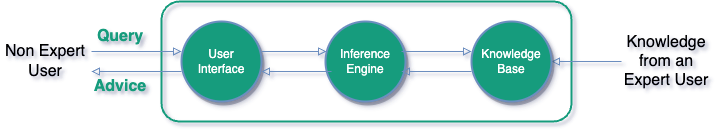
\includegraphics[scale=0.6]{images/Foundation-Architecture_Expert_System.drawio.png}
    \caption{\label{fig:es-archi} Architecture of an Expert System \cite{tripathi2011review} }
\end{figure}

Components of an expert system : 
\begin{itemize}
    \item \textbf{Knowledge base}: Facts and rules are represented here. It is made up of intrinsic facts relevant to the domain, methods, rules for solving problems and knowledge specific to the domain.
    \item \textbf{Inference engine}: this retrieves relevant information from the knowledge base, analyses it, and determines a solution that addresses the user's problem. To deduce new facts, the inference engine extracts rules from its knowledge base and applies them to known facts. In addition, debugging and explanation functions can be added to inference engines.
    \item \textbf{Learning and knowledge acquisition module}: The aim of this part is to enable the expert system to collect and store knowledge from various sources on an ongoing basis.
    \item \textbf{User interface}: Using this module, a non-expert user can communicate with the expert system and work out a solution.
    \item \textbf{The explanation module} helps the expert system to provide the user with a detailed explanation of how it arrived at a certain result.
\end{itemize}


\subsection{Semantic Web\label{sec:semweb}}
The Semantic Web is an expansion of the World Wide Web that intends to enable robots to comprehend and interpret the meaning of content on the internet \cite{shadbolt2006semantic, berners2023semantic, kim2003semantic}. It entails encoding data in a way that improves interconnectivity, connecting similar information, and enabling computerized processing. The objective is to improve information retrieval efficiency while also enabling more intelligent online apps and services.\\

In 2001, Tim Berners-Lee coined the term “Semantic Web” to describe the use of semantic technologies in data connectivity \cite{berners2023semantic}. The World Wide Web Consortium (W3C), founded by Berners-Lee, disseminates and supports a number of technical guidelines for the Semantic Web.\\

Improving the way computers understand data makes it easier to share data and enables it to be processed automatically. As Figure \ref{fig:sem-web-stack} shows, the \acrfull{owl}, \acrfull{sparql} and \acrfull{rdf} are the main standards on which semantic technology is developing. In contrast, in conventional information technology, meanings are hard-coded into application code and data at the design stage. \\

\begin{figure}[h]
    \centering
    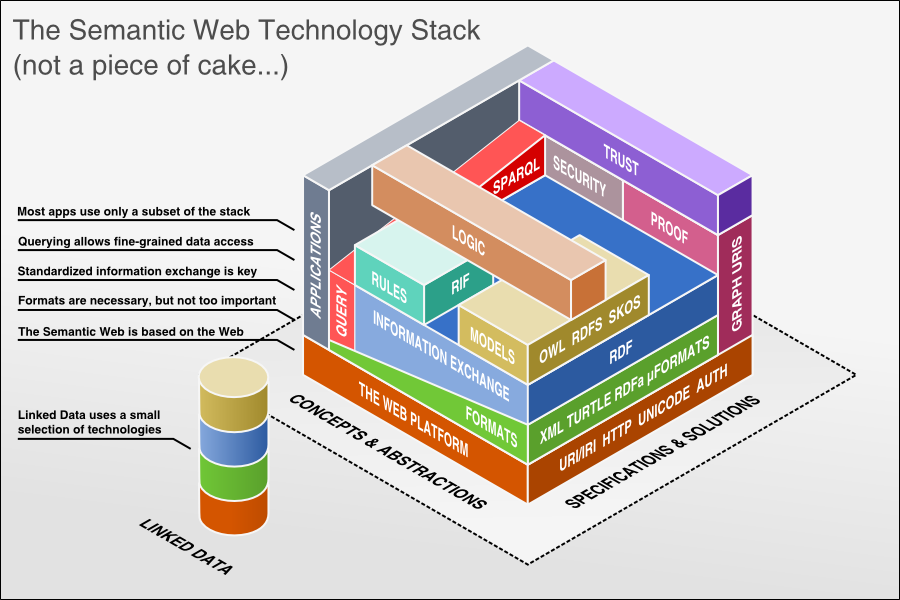
\includegraphics[scale=0.6]{images/foundation-sem-web-tech-stack.png}
    \caption{\label{fig:sem-web-stack} Semantic Web Technologies Stack \cite{semWebStack} }
\end{figure}


    \subsubsection{\acrshort{uri} and \acrshort{iri}}
        \paragraph{\acrfull{uri}}
        A \acrshort{uri} is a short string of characters that clearly identifies an abstract or physical resource on the Semantic Web \cite{de2016names}. The use of \acrshort{uri}s makes resources available through a number of naming systems and access mechanisms. A \acrshort{uri} can be used for location, identification, or both. There are two types of \acrshort{uri}: URLs and URNs. A \acrfull{url} is a subset of a \acrshort{uri} that indicates the location of a resource and how to retrieve it. A \acrfull{urn}, on the other hand, is used to identify an online resource without specifying how it will be retrieved.\\

        Semantic Web resource identifiers can be divided into a base \acrshort{uri} and a local name. In serialization, the base \acrshort{uri} is often shortened by a prefix defined at the beginning. Figure \ref{fig:uri-example} shows an example of a \acrshort{uri} and its decomposition with a prefix.\\

        \begin{figure}[h]
            \centering
            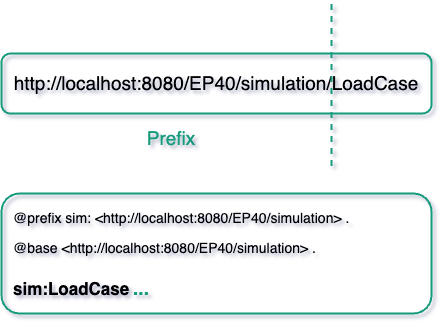
\includegraphics[scale=0.6]{images/Foundation-URI Decomposition.drawio.png}
            \caption{\label{fig:uri-example} Example of \acrshort{uri} and decomposition with prefix}
        \end{figure}

        
        \paragraph{\acrfull{iri}}
        \acrshort{iri} is an extension of the \acrshort{uri} that adapts to a global character set, whereas the \acrshort{uri} is limited to \acrshort{ascii} and has far fewer characters. \acrshort{iri}s enable the representation and communication of data-related knowledge in several languages. \acrshort{iri}s can be transformed into \acrshort{uri}s using percentage encoding, enabling backward compatibility.


    \subsubsection{\acrfull{rdf}}
    \acrshort{rdf} is a resource description framework developed by W3C. It is used in particular on the World Wide Web for data exchange. The \acrshort{rdf} data model allows data resources to be uniquely recognized and linked to other data resources for reading, analysis and action \textbf{decker2000framework}. 

    \acrshort{rdf} introduces several fundamental Semantic Web terms:

    \begin{itemize}
        \item A \textbf{resource} is anything that can be characterized by an \acrshort{rdf} declaration. \acrshort{uri}s ensure that resources are always uniquely named. Any physical thing or notion can be represented by a \acrshort{uri}, allowing \acrshort{rdf} to be used to describe different types of domains.
        \item A \textbf{“thing”} is either an individual object, called an instance, or a definition of a type of thing, called a class. 
        \item A \textbf{schema} is an abstract description of a set of objects. It consists of a hierarchical taxonomy that describes how the elements of the domain are classified. In \acrshort{rdf}, schemas are also known as terminology boxes (Tboxes). 
        \item A \textbf{property} is an attribute, feature, characteristic or connection that facilitates the description of a \acrshort{uri}. In the \acrshort{rdf} architecture, a property is also represented in the form of a \acrshort{uri}. It always has a precise meaning and determines the type of resource it can describe, known as the property domain, as well as the permitted values. It can also specify how it relates to other attributes. 
        \item \textbf{Axioms} are property declarations for schema classes, often known as Role Boxes (Rbox) in \acrshort{rdf}. They define the relationships between classes.
    \end{itemize}

    \acrshort{rdf} is a model based on \textbf{Triples}. Triples are built around \textbf{subject-predicate-object} relationships, and are the most common type of axiom. The predicate is a property or a relation; the subject is a “thing”. When the object is a thing, the property is called an \textbf{object property}. If the object is a literal, such as a character, integer or string, the property is called a \textbf{data property}. Once a triplet has been defined, it is referred to as a \textbf{statement} \cite{noy2001ontology}.\\

    Take, for example, this basic English sentence: “Germany is in Europe”. Table\ref{tab:rdf-example} shows how the sentence can be divided syntactically. If this statement were to be expressed visually, this could be done using the following directed graph, shown in Figure \ref{fig:rdf-example}.\\
    
    \begin{table}[h]
        \centering
	    \rowcolors{2}{teal!10}{white}
	    \begin{tabular}{ | m{4cm} | m{4cm} | m{4cm} | }
            \hline
            \rowcolor{teal!30} Subject & Predicate & Object \\
            
            \hline
            Germany  & is in & Europe\\
            
            \hline
        \end{tabular}
        \caption{\label{tab:rdf-example} RDF Syntactic division}
        \end{table}
        
    \begin{figure}[h]
        \centering
        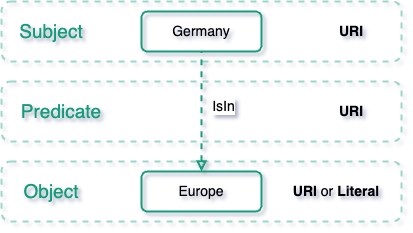
\includegraphics[scale=0.6]{images/Foundation-RDF Example.drawio.png}
        \caption{\label{fig:rdf-example}  RDF Graphical representation}
    \end{figure}

    \acrshort{rdf} uses the same techniques to demonstrate the links between subjects and objects. However, as explained earlier, to represent resources and features accurately on the web, they need to be assigned a unique \acrshort{uri}. To demonstrate the representation of the above example sentence as a triple, the \acrshort{uri}s of the resources and attributes are assumed to be those shown in Table\ref{tab:rdf-example-uri}.
    
    \begin{table}[h]
        \centering
	    {\rowcolors{2}{teal!10}{white}
	    \begin{tabular}{ | m{2.5cm} | m{2.5cm} | c | }
            \hline
            \rowcolor{teal!30} Entity & Role & URI \\
            
            \hline
            Germany  & Subject & $<http://example/resource/Germany>$\\
            
            \hline
            is in  & Predicate & $<http://example/resource/isIn>$\\
            
            \hline
            Europe  & Object & $<http://example/resource/Europe>$\\
            
            \hline
        \end{tabular}}
        \caption{\label{tab:rdf-example-uri} Example of URI Scheme}
    \end{table}

    \subsubsection{Linked Data Principles}
    Linked data is a way of representing and distributing structured data on the web. Data generated and structured according to Linked Data principles is machine-readable and connected to other data on the web. It uses conventional web technologies such as \acrshort{http}, \acrshort{rdf} and \acrshort{uri}, but not only does it provide human-readable data via web pages, it also makes it machine-readable \cite{bizer2008linked}. Linked data allows concepts, elements, events, people, places, etc. to be organized and linked together. There are many platforms on the web that make available a large amount of linked data and the relationships between them. These include WikiData, DBpedia and \acrfull{lov}.\\

    Tim Berners-Lee, the initiator and defender of the Semantic Web and linked data, established the four design principles of linked data back in 2006 \cite{bizer2008linked, bizer2011linked}.
    \begin{enumerate}
        \item Use \acrshort{uri}s to name objects.
        \item Use \acrshort{http} \acrshort{uri}s to provide useful information. 
        \item Use open standards such as \acrshort{rdf} and \acrshort{sparql} to provide meaningful information about what a name indicates when searched. 
        \item Include connections to other \acrshort{uri}s to allow them to find new information. 
    \end{enumerate}

    The more data is represented as linked data on the web, the greater the possibility of linking it to other linked data sources. For example, if a resource represented by a \acrshort{uri} in one data source is discovered in an existing linked data source (e.g., WikiData or DBpedia), it can be connected to a property such as \textbf{owl:sameAs} to extract further metadata and investigate links to other data resources \cite{bizer2008linked}.\\

    \subsubsection{Ontology}
    In the field of philosophy, ontology is a discipline that studies existence, the way in which knowledge, language, and perception are related to the nature of reality \cite{smith2012ontology}. It is concerned with the question of what entities exist and how they can be classified, ordered hierarchically and discriminated against. \\
    Since the mid-1970s, \acrshort{ai} researchers have realized that knowledge engineering is essential for developing large and powerful \acrshort{ai} systems \textbf{fensel2001ontologies}. \acrshort{ai} researchers suggested that they could develop new ontologies as computational models to enable certain types of automated reasoning, but their efforts were only moderately successful. In the 1980s, the \acrshort{ai} community began using the term ontology to describe both a theory of a modelled world and a component of knowledge-based systems \textbf{guarino1995formal}.\\
    An ontology captures the structure of a domain, i.e. the model and its constraints. In other words, an ontology is a structure for systematically storing and formalizing domain knowledge. Ontology schemas are created using two modelling languages, \acrfull{rdfs} and \acrfull{owl} \textbf{fensel2001ontologies}.\\

    Tim Berners-Lee \cite{kuck2004tim} defines an ontology as having the following properties: 
    \begin{enumerate}
        \item It must have a concise syntax.
        \item It must have well-defined semantics, making it possible to state correctly what is represented.
        \item It must have sufficient expressive capacity to convey human knowledge.
        \item It must have an effective, robust and simple reasoning process. 5. it must be capable of generating huge knowledge bases.
    \end{enumerate}


\subsection{Role of Semantic Technology in Systems Engineering}
In order to improve the efficiency of systems engineering processes, the integration of semantic technology appears to be a promising avenue \cite{hagedorn2020knowledge}. The application of semantic technology to simulation configuration in the automotive industry provides a more nuanced understanding of the relationships between simulation parameters, facilitating intelligent decision-making and configuration suggestion. Using \acrshort{rdf} standards, the metadata of many artifacts in a simulation can be merged into a single database. The database will include objects and information useful throughout the configuration process, uniformly represented as \acrshort{rdf} graphs. This integration allows \acrshort{sparql} to query the database, enabling complex queries to be managed.\\

This study aims to bridge the gap between traditional systems engineering methodologies and cutting-edge semantic technologies, providing a new perspective on the configuration processes that are essential for advancing simulation capabilities in the automotive sector. In the next chapter, an analysis of the “State of the Art” and “of Practice” will be made in order to have a more precise idea of the work already done on this subject.












\clearpage
\section{Related work\label{sec:relwork}}
This chapter presents the techniques and conclusions of the literature review. Firstly, an analysis will be made of the research already carried out on our subject. The methodology and reasoning behind the literature review will be presented, together with a summary of the results. Next, a comparison of current tools that are close to the objective of this thesis will be carried out.\\

    \subsection{State of the Art}
        \subsubsection{\acrfull{sms}}
        Systematic mapping is a strategy for creating a categorization system and organizing a specific topic of interest \cite{petersen2008systematic}. It is a research approach that involves examining current published research reports, evaluating them in depth and summarizing their methodology and conclusions. It is carried out in several stages, as shown in the \textbf{Figure \ref{fig:SysMapProcess}}, and results in a classification (mapping) of the articles studied.\\

        \begin{figure}[h]
            \centering
            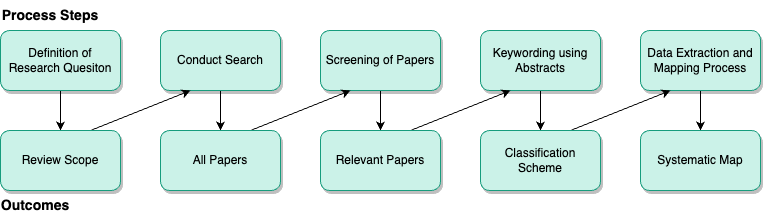
\includegraphics[scale=0.6]{images/RelatedWork-SysMapProcess.drawio.png}
            \caption{\label{fig:SysMapProcess}  The Systematic Mapping Process (\cite{petersen2008systematic})}
        \end{figure}

        First, the \textbf{\acrshort{sms}} research questions had to be identified, which enabled a preliminary search for relevant articles to be carried out. These research questions should be considered as sub-questions of those defined in \textbf{Section \ref{subsec:reseques}}. The information extracted from these articles was used to develop a set of keywords and a categorization system. Before examining the articles to determine their relevance to this work, the inclusion, and exclusion criteria must be established. On the basis of the results, the context, and aspect of the research were defined. The final stage is the data extraction and mapping procedure, which results in a systematic map \cite{petersen2008systematic, petersen2015guidelines}.\\

            \paragraph{Research questions\label{para:res-ques}}
            The research questions defined in \textbf{Section \ref{subsec:reseques}} provide a more concise definition of the issues raised by the subject of this thesis. However, in order to learn from existing methodologies and possibly adapt elements of their tool chain, we need to ask more specific questions in the context of our \acrshort{sms}. To demonstrate the relationship with our main research questions, these are repeated and for each one a corresponding structured mapping study question (\textbf{SMS\_Q}) is presented.

            \begin{itemize}
                \item Q1: What are the main challenges and limitations of current configuration processes for simulations in the automotive industry?
                    \begin{itemize}
                        \item \textbf{SMS\_Q1}: What are the most frequently cited challenges associated with current configuration practices for simulations in the automotive industry?
                    \end{itemize}


                \item Q2: How can semantic technology be used to support simulation configuration processes?
                    \begin{itemize}
                        \item \textbf{SMS\_Q2}: What are the key concepts and principles of semantic technology that can be applied to simulation configuration?

                        \item \textbf{SMS\_Q3}: How can semantic technologies enable the representation and management of simulation configuration knowledge in a structured and machine-interpretable way?
                    \end{itemize}
                    
                \item Q3: What are the requirements of a semantic-based configuration tool for automotive simulations?
                    \begin{itemize}
                        \item \textbf{SMS\_Q4}: What are the essential functionalities and features that a semantic-based configuration tool for automotive simulations should possess?
                    \end{itemize}


                \item Q4: What are the existing semantic technologies and standards applicable to the field of systems engineering and simulation configuration, and how can they be adapted to support simulation configuration processes?
                    \begin{itemize}
                        \item \textbf{SMS\_Q5}: What are the prominent semantic technologies and standards that are relevant to systems engineering and simulation configuration?

                        \item \textbf{SMS\_Q6}: In what ways can these exist semantic technologies and standards be adapted or integrated to effectively support simulation configuration processes in the automotive industry?
                    \end{itemize}

            \end{itemize}

            
            \paragraph{Search strings for search}
            \textbf{Table \ref{tab:keyw-syno}} shows the keywords obtained after the preliminary search.\\

            \begin{table}[h]
                \centering
        	    {\rowcolors{2}{teal!10}{white}
        	    \begin{tabular}{ | m{5.5cm} | m{9cm} | }
                    \hline
                    \rowcolor{teal!30} \textbf{Keywords} & \textbf{Synonyms} \\
                    
                    \hline
                    semantic technologies  & Ontologies, Knowledge graphs\\
                    
                    \hline
                    simulation data & Simulation knowledge\\
                    
                    \hline
                    Case-Based Reasoning  & Similarity-Based, Experience-Based, knowledge-Based Reasoning\\
                    
                    \hline
                    Rule-Based Reasoning  & \\
                    
                    \hline
                    Expert-System  & \\
                    
                    \hline
                    Computer Aided Engineering  & Computer Assisted Engineering\\
                    
                    \hline
                \end{tabular}}
                \caption{\label{tab:keyw-syno} Keywords and their Synonyms}
            \end{table}

            The keywords found were then searched for synonyms, related phrases and alternative spellings \cite{budgen2006performing}. As usual, Boolean logic was used to define a search string, combining alternative phrases with \textbf{“OR”} and linking terms with \textbf{“AND”}. The final search string is as follows:\\

            \begin{lstlisting}[language=XML, caption=Generated Query, label={lst:gen-query}]
"semantic technologies" 
OR ("Ontology" AND "Simulation")
OR ("simulation configuration process" OR "simulation configuration workflow" OR "simulation configuration knowledge")
OR (("Case-Based Reasoning" OR "Similarity-Based Reasoning" OR "Experience-Based Reasoning" OR "knowledge-Based Reasoning") AND "Simulation")
OR ("Rule-Based Reasoning" AND "Simulation")
OR ("Expert-System" AND "Simulation")
OR (("Computer Aided" OR "Computer Assisted") AND "engineering")
            \end{lstlisting}

            Once the search query was obtained, the search was carried out in 3 main platforms: \textbf{ACM}, \textbf{IEEE} and \textbf{ScienceDirect}. 


            \paragraph{Inclusion and Exclusion Criteria}
            In this section, the inclusion, and exclusion criteria will be defined. They allow certain restrictions to be imposed in order to obtain only useful and relevant results.

            \begin{itemize}
                \item Inclusion criteria:
                    \begin{itemize}
                        \item \textbf{IC1}: Papers with keywords that match our query (at the level of their title or abstract).
                    \end{itemize}

                \item Exclusion criteria:
                    \begin{itemize}
                        \item \textbf{EC1\label{EC1}} : Papers whose abstract content does not focus on one of the following themes:
                            \begin{itemize}
                                \item semantic technologies,
                                \item expertise systems
                                \item case-based reasoning
                                \item rule-based reasoning
                            \end{itemize}

                        \item \textbf{EC2\label{EC2}} : Papers not written in English or German

                        \item \textbf{EC3\label{EC3}} : Papers not publicly accessible from the chosen platforms
                    \end{itemize}
            \end{itemize}

            One point to emphasize is that in most mapping studies, an exclusion criterion is also defined in relation to the date of publication. This makes it possible to limit the period of publication of the results (e.g., 2002 — now). But this thesis revolves very much around case-based and rule-based reasoning, which are very old artificial intelligence techniques compared with modern methods.

            
            \paragraph{Classification Scheme}
            In this section, we follow the approach introduced by Bailey \cite{hill2019systematic} and described in \textbf{Figure \ref{fig:BuildClassSchem}}. Here, classification is based mainly on \textbf{keywording}. Keywording is a method of speeding up the classification process by extracting keywords from the abstracts of selected articles \cite{petersen2008systematic}. In this way, the context of each contribution can be easily obtained. Once this stage has been completed, an examination of the relevant keywords in each article provides an in-depth understanding of the nature and importance of the research \cite{petersen2008systematic}. \\
            This knowledge is used to create categories to classify all the articles. When the quality of abstracts is insufficient to allow the selection of significant keywords, it may be necessary to read the introduction and conclusion of an article.

            \begin{figure}[h]
                \centering
                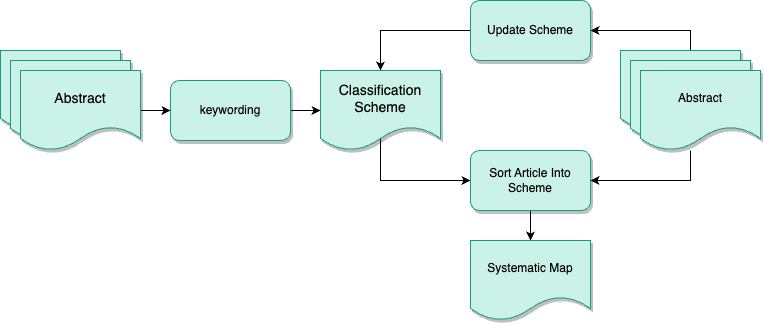
\includegraphics[scale=0.6]{images/RelatedWork-Build-Class-Schem.drawio.png}  \caption{\label{fig:BuildClassSchem}  Building the Classification Scheme \cite{petersen2008systematic}}
            \end{figure}

           In the context of this research, three facets have been identified. The first facet summarizes the subject of our thesis (i.e., Semantic Technologies usage). \textbf{Table \ref{tab:sem-tec-usage}} shows the possible values of this facet. The other two facets are more commonly used to group research contributions and can therefore be integrated \cite{petersen2008systematic, wieringa2006requirements}: research type and contribution.\\
            The research facet represents the research technique used in the study; these approaches are domain-neutral and can be used without change (\textbf{Table \ref{tab:contri-ty-face}}).\\
            The third facet, the contribution facet, documents the contribution made in terms of, for example, process, method or tool, etc. (\textbf{Table \ref{tab:research-ty-face}}).\\
            The results of the \acrshort{sms} are presented below. The appendix contains the full results.

        
            \begin{table}[h]
                \centering
        	    {\rowcolors{2}{teal!10}{white}
        	    \begin{tabular}{ | m{14.5cm} | }
                    \hline
                    \rowcolor{teal!30} \textbf{Category} \\
                    
                    \hline
                    Case-based reasoning\\
                    
                    \hline
                    Rule-based reasoning\\
                    
                    \hline
                    Expertsystem\\
                    
                    \hline
                    Knowledge representation\\
                    
                    \hline
                \end{tabular}}
                \caption{\label{tab:sem-tec-usage} Semantic Technologies Usage}
            \end{table}

            \begin{table}[h]
                \centering
        	    {\rowcolors{2}{teal!10}{white}
        	    \begin{tabular}{ | m{2cm} | m{12.5cm} | }
                    \hline
                    \rowcolor{teal!30} \textbf{Category} & \textbf{Description} \\
                    
                    \hline
                    Metric  & Papers classified under Metric contributions focus on the creation or evaluation of specific measurement criteria or metrics within a certain context.\\
                    
                    \hline
                    Tool & Papers classified under Tool contributions describe the development, improvement, or assessment of software tools meant to meet specific difficulties in a certain domain.\\
                    
                    \hline
                    Model  & Papers in the Model contribution category contribute to the creation or enhancement of conceptual or computational models in a given topic.\\
                    
                    \hline
                    Method  & Method contributions concentrate on the development, improvement, or assessment of new research methodology or approaches.\\
                    
                    \hline
                    Process  & Papers in the Process contribution category focus on the design, assessment, or improvement of specific processes or workflows.\\
                    
                    \hline
                \end{tabular}}
                \caption{\label{tab:contri-ty-face} Contribution Type Facet}
            \end{table}

            \begin{table}[h]
                \centering
        	    {\rowcolors{2}{teal!10}{white}
        	    \begin{tabular}{ | m{2cm} | m{12.5cm} | }
                    \hline
                    \rowcolor{teal!30} \textbf{Category} & \textbf{Description} \\
                    
                    \hline
                    Validation Research  & The techniques explored are innovative and have not yet been used in practice. Experiments, or laboratory work, are one example of a technique employed.\\
                    
                    \hline
                    Evaluation Research & Techniques are put into practice, and their effectiveness is evaluated. That is, it is demonstrated how the approach is applied in practice (solution implementation) and what the implications are in terms of advantages and downsides (implementation assessment). This involves identifying difficulties in the industry.\\
                    
                    \hline
                    Solution Proposal  & A solution to a problem is given; the solution may be unique or a major expansion of an existing approach. A tiny example or a strong line of reasoning demonstrates the solution's potential benefits and application.\\
                    
                    \hline
                    Philosophical Papers  & These publications provide a new way of looking at existing objects by arranging the area in the form of a taxonomy or conceptual framework.\\
                    
                    \hline
                    Opinion Papers  & These articles offer the author's own view on whether a particular approach is excellent or terrible, or how things should have been done. They do not rely on previous work or research methods.\\
                    
                    \hline
                    Experience Papers  & Experience papers describe what and how something was done in practice. It must be based on the author's real experiences.\\
                    
                    \hline
                \end{tabular}}
                \caption{\label{tab:research-ty-face} Research Type Facet}
            \end{table}

    
        \subsubsection{Result}
        This section presents the results of the mapping study. \textbf{Paragraph \ref{para:sms_analysis}} provides an analysis of the results obtained, followed by in-depth answers to the research questions defined in \textbf{Paragraph \ref{para:sms_ans_rq}}.

            \paragraph{Results of Database Search}
            The predefined keywords and the \hyperref[EC2]{\textbf{EC2}} criterion were used to obtain a total of \textbf{26270} research publications. These are classified as, \textbf{25175} for IEEE, \textbf{203} for ACM and \textbf{892} for ScienceDirect. Due to the \hyperref[EC3]{\textbf{EC3}} exclusion criterion, the number of articles obtained fell to \textbf{389} for IEEE, \textbf{203} for ACM and \textbf{125} for ScienceDirect. For a total of \textbf{717} articles. The \hyperref[EC1]{\textbf{EC1}} exclusion criterion was then used to reduce the number of relevant articles even further. This resulted in a total of \textbf{24 articles}.\\
            This was followed by a manual keyword-by-keyword search, which produced better quality results. Manual target searching has been shown to produce high quality search results when combined with searches of digital libraries \cite{petersen2008systematic}. We integrated manual target searches from other platforms, such as Google Scholar. This resulted in 27 additional articles. \textbf{Table \ref{tab:rel-papers}} shows the list of articles selected, classified by publication date. This list was filtered on the basis of inclusion and exclusion criteria, and duplicate articles from different platforms were removed.\\

            
        	    {\rowcolors{2}{teal!10}{white}
        	    \begin{longtable}{ | m{1cm} | m{1.5cm} | m{12cm} | }
                    \caption{\label{tab:rel-papers} Relevant papers, ordered by year of appearance}\\
                    \hline
                    \rowcolor{teal!30} \textbf{ID} &\textbf{Year} &\textbf{Title} \\
                    \hline
                    \endfirsthead
                    
                    \hline
                    \textbf{A28} &1992 &Fallbasiertes Schließen \\ %\cite{althoff1992fallbasiertes} \\
                    \hline
                    \textbf{A17} &1995 &Case based reasoning \\ %\cite{richter2016case} \\
                    \hline
                    \textbf{A26} &1995 &Fallbasiertes Schließen zur Kreditwürdigkeitsprüfung \\ %\cite{wilke1995fallbasiertes} \\
                    \hline
                    \textbf{A19} &2001 &A Tutorial on Case Based Reasoning \\ %\cite{main2001tutorial} \\
                    \hline
                    \textbf{A5} &2002 &Ontology-Driven Induction of Decision Trees at Multiple Levels of Abstraction \\ %\cite{zhang2002ontology} \\
                    \hline
                    \textbf{A18} &2003 &R5 model for case-based reasoning \\ %\cite{finnie2003r5} \\
                    \hline
                    \textbf{A20} &2003 &From Case-based Reasoning to Problem-based Learning \\ %\cite{eshach2003case} \\
                    \hline
                    \textbf{A3} &2006 &Using Ontologies for Simulation Modeling \\ %\cite{benjamin2006using}\\
                    \hline
                    \textbf{A30} &2007 &Using ontologies for simulation integration \\ %\cite{benjamin2007using}\\
                    \hline
                    \textbf{A4} &2008 &SemTree: ontology-based decision tree algorithm for recommender systems \\ %\cite{bouza2008semtree} \\
                    \hline
                    \textbf{A31} &2008 &Clustering with case-based reasoning for wireless sensor network \\ %\cite{wang2008clustering} \\
                    \hline
                    \textbf{A12} &2010 &Ontology-Based Context Representation and Reasoning Using OWL and SWRL \\ %\cite{liu2010ontology} \\
                    \hline
                    \textbf{A25} &2010 &Problem Solving by Case-Based Reasoning \\
                    \hline
                    \textbf{A27} &2010 &Problem Solving by Case-Based Reasoning 2 \\
                    \hline
                    \textbf{A49} &2010 &Using ontologies for the federated simulation of critical infrastructures \\ %\cite{tofani2010using} \\
                    \hline
                    \textbf{A21} &2011 &Case-Based Reasoning Research and Development \\ %\cite{wiratunga2011case} \\
                    \hline
                    \textbf{A11} &2012 &A recommendation system based on domain ontology and SWRL for anti-diabetic drugs selection \\ %\cite{chen2012recommendation} \\
                    \hline
                    \textbf{A6} &2013 &Ontology Enhancement through Inductive Decision Trees \\ %\cite{chen2012recommendation} \\
                    \hline
                    \textbf{A29} &2013 &Developing a real-time inference approach for rule-based reasoning systems \\ %\cite{qiao2013developing} \\
                    \hline
                    \textbf{A16} &2014 &The Collaborative Agile Knowledge Engine CAKE \\ %\cite{bergmann2014collaborative} \\
                    \hline
                    \textbf{A46} &2014 &Domain Ontologies Integration for Virtual Modelling and Simulation Environments \\ %\cite{smirnov2014domain} \\
                    \hline
                    \textbf{A48} &2014 &An Ontology Framework for Rule-based Inspection of eeBIM-systems \\ %\cite{kadolsky2014ontology}\\
                    \hline
                    \textbf{A50} &2014 &Hybrid Fuzzy-ontological Project Framework of a Team Work Simulation System \\ %\cite{orlowski2014hybrid} \\
                    \hline
                    \textbf{A52} &2014 &Human System Integration Ontology: Enhancing Model Based Systems Engineering to Evaluate Human-system Performance \\ %\cite{orellana2014human}\\
                    \hline
                    \textbf{A51} &2015 &Decision Support in Production Planning of Precast Concrete Slabs Based on Simulation and Learning from Examples \\ %\cite{konczak2015decision} \\
                    \hline
                    \textbf{A7} &2016 &Development of an ontology-based configuration management system \\ %\cite{na2016development}\\
                    \hline
                    \textbf{A9} &2016 &Automatic CAD model retrieval based on design documents using semantic processing and rule processing \\ %\cite{jeon2016automatic}\\
                    \hline
                    \textbf{A13} &2017 &Conversational Process-Oriented Case-Based Reasoning \\ %\cite{zeyen2017conversational}\\
                    \hline
                    \textbf{A34} &2017 &Case-Based Reasoning for Product Style Construction and Fuzzy Analytic Hierarchy Process Evaluation Modeling Using Consumers Linguistic Variables \\ %\cite{wang2017case}\\
                    \hline
                    \textbf{A45} &2017 &Development of Knowledge-Expandable Ontology-Based Expert System for Process Planning in Cold Forging of Flange Nuts \\ %\cite{chang2017development}\\
                    \hline
                    \textbf{A8} &2018 &An ontology-based product design framework for manufacturability verification and knowledge reuse \\ %\cite{li2018ontology}\\
                    \hline
                    \textbf{A10} &2018 &Improving integrated product design using SWRL rules expression and ontology-based reasoning \\ %\cite{abadi2018improving}\\
                    \hline
                    \textbf{A14} &2019 &ProCAKE: A Process-Oriented Case-Based Reasoning Framework \\ %\cite{bergmann2019procake}\\
                    \hline
                    \textbf{A22} &2019 &Modeling CBR using Python for Football Matches \\ %\cite{sawalkar2019modeling} \\
                    \hline
                    \textbf{A38} &2019 &An Adaptive Model for Identification of Influential Bloggers Based on Case-Based Reasoning Using Random Forest \\ %\cite{asim2019adaptive} \\
                    \hline
                    \textbf{A23} &2020 &A Simple Approach to Case-Based Reasoning in Knowledge Bases \\ %\cite{das2020simple} \\
                    \hline
                    \textbf{A32} &2020 &A Novel Case Base Reasoning and Frequent Pattern Based Decision Support System for Mitigating Software Risk Factors \\ %\cite{asif2020novel} \\
                    \hline
                    \textbf{A39} &2020 &A Novel Optimized Case-Based Reasoning Approach With K-Means Clustering and Genetic Algorithm for Predicting Multi-Class Workload Characterization in Autonomic Database and Data Warehouse System \\ %\cite{shaheen2020novel}\\
                    \hline
                    \textbf{A43} &2020 &A Similarity Measure in Formal Concept Analysis Containing General Semantic Information and Domain Information \\ %\cite{wang2020similarity} \\
                    \hline
                    \textbf{A2} &2021 &OSMO: Ontology for simulation, modelling, and optimization \\ %\cite{horsch2021osmo} \\
                    \hline
                    \textbf{A15} &2021 &Improving Similarity-Based Retrieval Efficiency by Using Graphic Processing Units in Case-Based Reasoning \\ %\cite{malburg2021improving} \\
                    \hline
                    \textbf{A35} &2021 &Exploiting Ontology Recommendation Using Text Categorization Approach \\ %\cite{sarwar2020exploiting} \\
                    \hline
                    \textbf{A36} &2021 &On Approximation of Concept Similarity Measure in Description Logic ELH With Pre-Trained Word Embedding \\ %\cite{racharak2021approximation}\\
                    \hline
                    \textbf{A37} &2021 &Semankey: A Semantics-Driven Approach for Querying RDF Repositories Using Keywords \\ %\cite{abad2021semankey} \\
                    \hline
                    \textbf{A40} &2021 &Multivariable Case Adaptation Method of Case-Based Reasoning Based on Multi-Case Clusters and Multi-Output Support Vector Machine for Equipment Maintenance Cost Prediction \\ %\cite{lin2021multivariable} \\
                    \hline
                    \textbf{A41} &2021 &Predicting Influential Blogger’s by a Novel, Hybrid and Optimized Case Based Reasoning Approach With Balanced Random Forest Using Imbalanced Data \\ %\cite{asim2020predicting}\\
                    \hline
                    \textbf{A47} &2021 &ORVIPO: An Ontological Prototype for Modeling 3D Scenes in Operating Rooms \\ %\cite{jaziri2021orvipo} \\
                    \hline
                    \textbf{A42} &2022 &F-CBR: An Architecture for Federated Case-Based Reasoning \\ %\cite{jaiswal2022f} \\
                    \hline
                    \textbf{A44} &2022 &An Interval Type-2 Fuzzy Ontological Similarity Measure \\ %\cite{adel2022interval} \\
                    \hline
                    \textbf{A1} &2023 &Simulation Data goes Ontology \\ %\cite{spelten2023simulation} \\
                    \hline
                    \textbf{A33} &2023 &A Generation and Repair Approach to Scheduling Semiconductor Packaging Facilities Using Case-Based Reasoning \\ %\cite{park2023generation} \\
                    \hline
                \end{longtable}}%%
            
            Here, a bubble chart has been used to present the frequencies, as shown in \textbf{Figure \ref{fig:viz-smb}}. Essentially, these are two x-y scatter plots whose bubbles represent category crossovers. The size of a bubble is proportional to the number of items in the category pair corresponding to its coordinates. The same concept is repeated, in separate quadrants of the same figure, to demonstrate the intersection with the third aspect. In the case of this thesis, bubble charts are more useful for analysis than frequency tables. It is simpler to evaluate many facets at once, although summary data can still be provided for specific facets. It's also more effective at providing a quick overview of a domain, thus acting as a map. In addition to this diagram, \textbf{Figure \ref{fig:distro-art}} presents sector diagrams showing the statistical distribution of each of our facet points.

            
            \begin{figure}[h]
            \centering
            \bubbleplot[%
                width=1cm,
                height=1cm,
                xmin=-7,
                xmax=8,
                ylabel="Semantic Technologies usage",
                meta=nbr,
                x field=x,
                enlarge y limits=0.3,
                x index field=ix,
                y field=y,
                y index field=iy,
                year field=years,
                year x shift=1cm,
                year y shift=0cm,
                year padding=0,
                x left label="Contribution Type Facet",
                x left label shift=4cm,
                x right label="Research Type Facet",
                x right label shift=0cm,
            ]{assets/MappingStud.csv}{1992, 1995, 2001, 2002, 2003, 2006, 2007, 2008, 2010, 2011, 2012, 2013, 2014, 2015, 2016, 2017, 2018, 2019, 2020, 2021, 2022, 2023}
            \caption{\label{fig:viz-smb}  Visualization of a Systematic Map as a Bubble Plot (Each Color Represent Different Years of Publication)}
            \end{figure}

            \begin{figure}[h]
                \centering
                \begin{subfigure}[b]{0.45\textwidth}
                    \centering
                    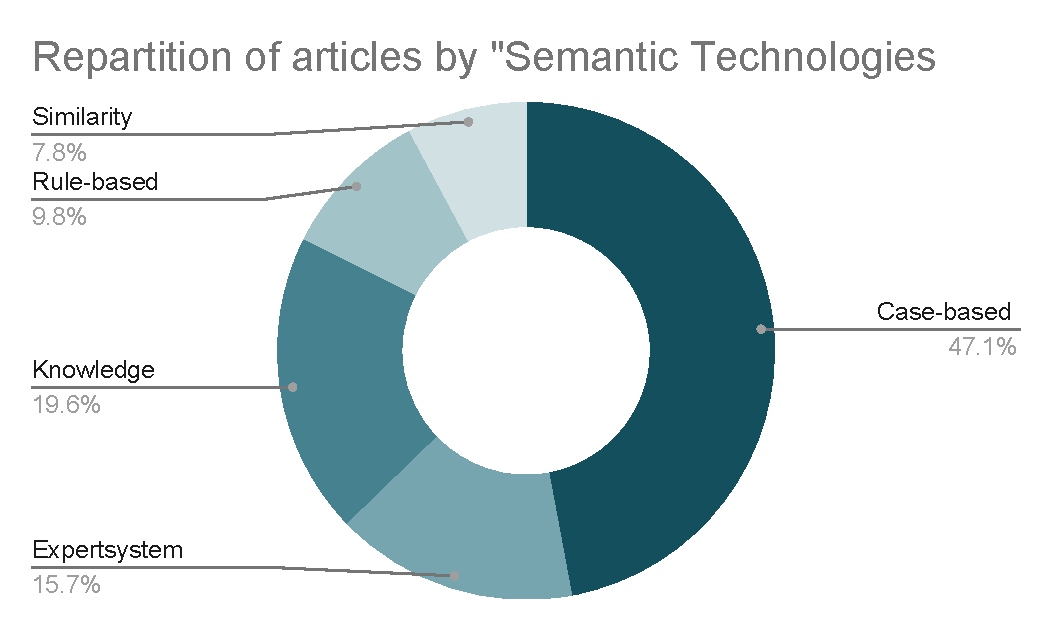
\includegraphics[width=\textwidth]{images/Repartition_by_Semantic_Technologies_usage.pdf}
                \end{subfigure}
                \begin{subfigure}[b]{0.45\textwidth}
                    \centering
                    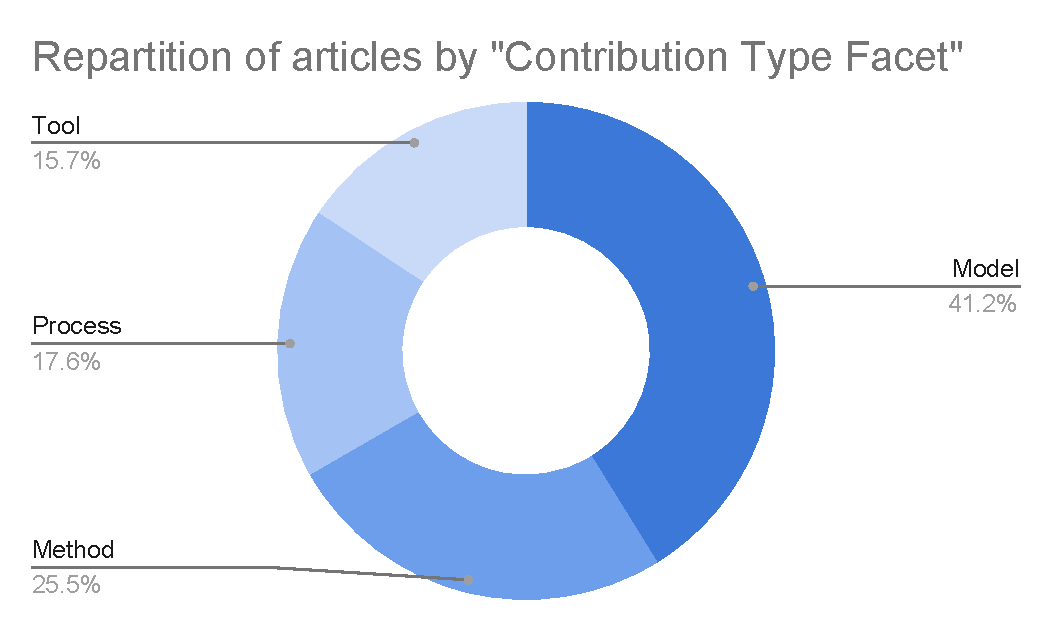
\includegraphics[width=\textwidth]{images/Repartition_by_Contribution_Type_Facet.pdf}
                \end{subfigure}
                \begin{subfigure}[b]{0.45\textwidth}
                    \centering
                    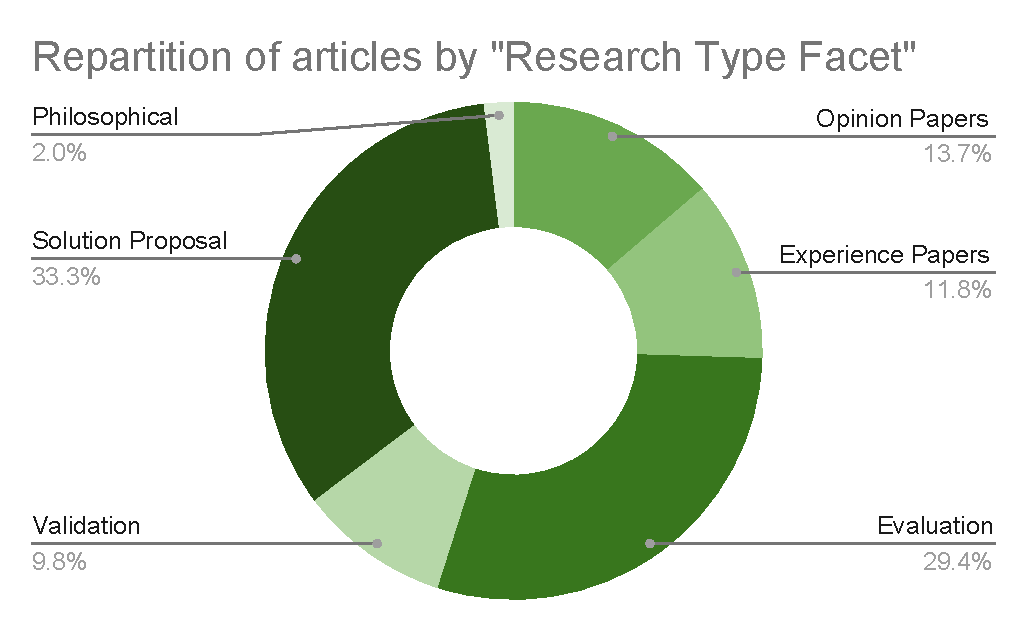
\includegraphics[width=\textwidth]{images/Repartition_by _Research_Type_Facet.pdf}
                \end{subfigure}
                \caption{\label{fig:distro-art} Distributions of the Articles}
            \end{figure}
            
            \paragraph{Analysis\label{para:sms_analysis}}
            The mapping study shows that the use of semantic technologies in engineering goes back many years. In particular, these technologies are used to represent concepts and knowledge, and to set up expertise systems. These systems can be based on rule-based or case-based reasoning.\\
            
            In terms of type of contribution, the vast majority of articles found (41.5\%) were models. This shows that the use of semantic technologies in systems engineering remains largely experimental. Numerous authors propose ideas for integrations that could more or less work \cite{benjamin2007using, tofani2010using, benjamin2006using, bouza2008semtree}. 25.5\% and 17.6\% represent the percentage of articles on Methods and Processes, respectively. In the them, authors describe and evaluate solutions to specific problems. Only 15.7\% of articles are dedicated to tools. This shows that very little software exists for the creation and integration of semantic technologies in engineering.\\
            As far as the type of research is concerned, 33.3\% of the articles focus on solution proposals and 29.4\% on research evaluations. In other words, each paper was prepared as part of a project addressing a specific problem. A remedy was then proposed, and usually a small case study was studied. This demonstrates the popularity of these technologies with researchers. But from the other statistics it can be concluded that their use is still in the testing phase and their adoption is still timid.\\

            The next step in our analysis is to interpret the figures according to how semantic technologies are used.\\
            Starting with knowledge representation, there are few tools in use. As presented in \cite{chen2012recommendation, abadi2018improving, liu2010ontology}, the tool generally used to create or maintain ontologies is “Protégé” and there is no regular procedure for setting up ontologies \cite{noy2001ontology}. This is why very few articles are based on a step-by-step presentation of the process. The team behind “Protégé” has nevertheless put together a set of best practices to follow \cite{noy2001ontology} in order to work as optimally as possible with their software. There are, however, articles that show how to create an ontology and the steps to follow \cite{sure2002methodology, li2018ontology}, but these are mostly domain-specific. \\

            When creating an ontology, it is possible to define constraints and rules that will be used by reasoners to perform inferences \cite{noy2001ontology}. These rules can be further defined using \acrfull{swrl} \cite{liu2010ontology, abadi2018improving}. This ontological language is based on \acrshort{owl} and, thanks to the principle of \acrfull{fol}, allows conditions to be defined, as well as the result if they are verified or not. A number of tools, such as JavaDON \cite{jovanovic2005achieving} or the "SWRLTab" plugin for “Protégé” \cite{liu2010ontology}, make it easy to define these rules. As demonstrated in \cite{li2018ontology, jeon2016automatic, na2016development}, the process of creating these rules is fairly standard and requires only a deep understanding of the relationships and interdependencies between the various elements of the ontology.\\

            Alongside rule-based reasoning, there is also case-based reasoning. The latter is used in the field of artificial intelligence \cite{wilke1995fallbasiertes, althoff1992fallbasiertes}, but is becoming less and less popular, being replaced by deep learning and neural networks \cite{wiratunga2011case}. In the field of engineering, there are numerous model proposals and experimental procedures, which show how this reasoning could be used to solve specific problems. Nevertheless, it remains very popular with companies for assisting employees in making decisions based on previous decisions present in archives \cite{eshach2003case}. Compared with other \acrshort{ai} techniques, \acrshort{cbr} considerably reduces the work involved in gathering and representing knowledge, which is undoubtedly one of the main reasons for the commercial success of \acrshort{cbr} applications \cite{benjamin2006using, wiratunga2011case}. Tools for performing case-based reasoning are few and \textbf{fairly old}. They include ProCake, myCBR, jCOLIBRI and others.\\

            When it comes to case-based reasoning, much of the research focuses on how similarity values between elements can be calculated. As shown in the articles \cite{shaheen2020novel, chen2012recommendation, wang2020similarity, malburg2021improving, racharak2021approximation, adel2022interval} there are numerous algorithms for calculating similarity between values depending on their type.\\

            Both rules- and case-based reasoning are integrated into expertise systems \cite{lin2021multivariable}. As presented in \textbf{Section \ref{subsec:exp-sys}}, these systems support users in carrying out specific tasks based on the knowledge provided by experts. The basic architecture of how these systems are structured is straightforward, but their implementation is generally company-specific. Tools such as JavaDON or Jess propose procedures to follow in order to set up such systems. Unfortunately, these studies were carried out many years ago, and the tools presented are no longer really maintained and updated.\\

            To sum up, semantic technologies are used in a variety of fields, including engineering. The ontologies they define enable the creation of data graphs that can be understood by machines (reasoning). They can also be used to define rules about the relationships and properties of elements present in the graph. These rules can be used for inference and reasoning. Another use for ontologies is case-based reasoning. Information from previous cases (data on the configurations of simulations carried out in the past) can be represented in an ontology, and thanks to the particularities of ontologies, a similarity calculation can be carried out to propose possible solutions to users. Both of these approaches have been successful in the professional world, but are unfortunately increasingly being replaced by artificial intelligence and modern methods such as deep learning and decision trees.\\

            
            \paragraph{Answering research questions\label{para:sms_ans_rq}}
            The primary aim of this mapping study is to identify research gaps, provide an overview of the approaches employed, and outline what can be expected from the use of the aforementioned tools. The answers to the questions defined in \textbf{Section \ref{para:res-ques}} are as follows.\\

            \textbf{SMS\_Q1}: What are the most frequently cited challenges associated with current simulation configuration practices in the automotive industry?
            \begin{quote}
                There are many challenges to highlight in the various collected articles related to simulation. The most common being:

                \begin{itemize}
                    \item \textbf{The complexity} \cite{park2023generation, spelten2023simulation} : Modern systems are increasingly complex, with many interacting components. Setting up simulations for large-scale systems can be difficult due to the sheer number of variables, dependencies, and interactions involved. This leads to concerns about traceability. Individual configuration changes can often have a significant influence on overall system performance, complicating troubleshooting and analysis.
                    \item \textbf{The standardization} \cite{spelten2023simulation, horsch2021osmo} : The absence of standardized simulation procedures and formats, units and naming standards between different tools and teams poses compatibility problems and makes it difficult to share simulations.
                    \item \textbf{Lengthy setup times} \cite{horsch2021osmo}: Setting up simulations often requires extensive manual configuration of tools and parameters, which is time-consuming, error-prone, and inconsistent.
                    \item \textbf{Limited reusability} \cite{horsch2021osmo, spelten2023simulation}: It can be difficult to develop simulation configurations that can be easily adapted to different circumstances and reused for several projects. It is essential to ensure that the configuration is flexible and that no major reworking is required for each use case.\\
                \end{itemize}
            \end{quote}

            \textbf{SMS\_Q2}: What are the key concepts and principles of semantic technology that can be applied to simulation configuration?
            \begin{quote}
                From the above problems, it is clear that the formalization of the elements and metadata of a simulation is a fairly critical point. It ensures collaboration between different players and the sustainability of previous simulations. This problem could be solved using ontologies \cite{benjamin2006using, benjamin2007using}. By setting up an ontology for simulations, it is possible to define standards for names and units of measurement. It is also possible to define the interdependent relationships between the various elements of simulations, or the rules to be followed when assigning values to parameters.\\
            \end{quote}

            \textbf{SMS\_Q3}: How can semantic technologies enable the representation and management of simulation configuration knowledge in a structured and machine-interpretable manner?
            \begin{quote}
                As mentioned above, ontologies represent a promising means of standardization. By creating an ontology, a knowledge tree is established. To target the problems associated with the configuration process, the elements required to configure a simulation must first be integrated into the ontology. The next step is to define the possible attribute values of these elements, as well as their interdependent relationships.\\
            \end{quote}

            \textbf{SMS\_Q4}: What are the essential functionalities and features that a semantic-based configuration tool for automotive simulations should possess?
            \begin{quote}
                A semantics-based configuration tool for simulations should have certain capabilities and features critical to successfully solving the complicated simulation design problems discussed above. Ideally, such a tool should include the following crucial features:
                \begin{itemize}
                    \item \textbf{Data Management}: Use ontologies to specify the meaning and relationships between data, promoting consistency and understanding \cite{benjamin2006using}.
                    \item \textbf{Semantic search and filtering}: Locate particular configuration items or variants using semantic attributes and connections \cite{abad2021semankey}.
                    \item \textbf{Version control and branching}: manage multiple configuration versions while enabling comparison, rollback and merge \cite{na2016development, spelten2023simulation}.
                    \item \textbf{Impact analysis}: Estimate the effects of modifications to individual configuration components on overall simulation results \cite{na2016development}.
                    \item \textbf{Version control with user access management}: Facilitate cooperation by controlling user access to different versions of the configuration.
                    \item \textbf{Annotation and documentation}: Allow users to annotate and record specific configuration choices and their justifications.
                    \item \textbf{Reusable configuration repository}: Templates let you save and distribute frequently used configurations for easy reuse.
                    \item \textbf{Integration with knowledge management systems}: connect to existing knowledge bases to document and share best practices and lessons learned.
                    \item \textbf{Scalability and performance}: manage complex parameters and large data sets efficiently.\\
                \end{itemize}
            \end{quote}

            \textbf{SMS\_Q5}: What are the prominent semantic technologies and standards that are relevant to systems engineering and simulation configuration?
            \begin{quote}
                Semantic technologies such as RDFS, OWL, SPARQL, and many others are therefore of crucial importance \cite{benjamin2006using}.\\
            \end{quote}

            \textbf{SMS\_Q6}: In what ways can these existing semantic technologies and standards be adapted or integrated to effectively support simulation configuration processes in the automotive industry?
            \begin{quote}
                The integration of these technologies could be achieved by setting up an expert-system \cite{happel2006applications}. This system could use knowledge from experts stored in an ontology. Then, thanks to rules defined in the ontology and case reasoning, the expertise system will be able to assist the user by means of an inference unit (reasoner).  \textbf{Figure \ref{fig:es-archi}} shows the architecture of an expertise system.\\
            \end{quote}
        
    \subsection{State of Practice}
        \subsubsection{Semantic Web Technologies\label{sec:semtec}}
        Semantic technology is a set of approaches, tools, and strategies that offer sophisticated mechanisms for enhancing data in a domain with explicit meanings, making it understandable to computers. By creating data models known as ontologies, semantic web technologies represent an area of interest with a high degree of abstraction.\\ 
        
            \paragraph{RDF's Serializations}
                Unlike other data models, \acrshort{rdf} data models do not rely on a single serialization syntax. Triples in an \acrshort{rdf} dataset can be serialized in a number of ways \cite{martinez2012exchange}, and some of the most common serialization methods are : 

                \begin{itemize}
                    \item \textbf{RDF/XML}: RDF/XML is the most widely used serialization format for RDF in the W3C recommendations. RDF/XML is an XML-style tree document with a graph based on triples, which makes it theoretically difficult and verbose. 
                    \item \textbf{Notation3 (.n3)}: Unlike R/XML, N3 syntax is more concise and easier to understand because it is closer to the subject-predicate-object paradigm of \acrshort{rdf}. 
                    \item \acrfull{json} for Linking Data (JSON-LD) is a relatively new, user-friendly format. It combines web syntax (\acrshort{json}) with \acrshort{rdf} principles \cite{grlicky2005overview}. 
                    \item \textbf{Turtle}: The Turtle syntax is the successor to the N3 syntax, allowing more concise encoding of \acrshort{rdf} data.
                \end{itemize}

                \textbf{Listing \ref{lst:rdf-xml}}, \textbf{Listing \ref{lst:rdf-turtle}} and \textbf{Listing \ref{lst:rdf-json-ld}} show the serializations of a single example in different formats (RDF/XML, Turtle, JSON-LD) and \textbf{Figure \ref{fig:rdf-xml-example}} shows the graphical representation in RDF/XML. As you can see, the “turtle” syntax uses namespace prefixes to provide a more concise and clear syntax. It can also be used to describe lists of predicates or objects. There are also various serialization syntaxes for representing \acrshort{rdf}. However, due to its short structure and readability, the “turtle” syntax is used in this thesis for ontology development.\\
            
                \begin{figure}[H]
                    \centering
                    
\includegraphics[scale=0.6]{images/Foundation-RDF XML.drawio.png}
                    \caption{\label{fig:rdf-xml-example}  Graph Example in RDF/XML}
                \end{figure}

                \begin{lstlisting}[language=XML, caption=Example of RDF Serialization in RDF/XML, label={lst:rdf-xml}]
<?xml version="1.0" encoding="utf-8" ?>
<rdf:RDF xmlns:rdf="http://www.w3.org/1999/02/22-rdf-syntax-ns#"
            xmlns:ns0="http://dbpedia.org/ontology/">

    <rdf:Description rdf:about="http://dbpedia.org/resource/Pluto">
        <ns0:discovered>1930</ns0:discovered>
        <ns0:discoverer rdf:resource="http://dbpedia.org/resource/Clyde_Tombaugh"/>
    </rdf:Description>
</rdf:RDF>
                \end{lstlisting}

                \begin{lstlisting}[caption=Example of RDF Serialization in Turtle, label={lst:rdf-turtle}]
@prefix ns0: <http://dbpedia.org/ontology/> .

<http://dbpedia.org/resource/Pluto>
  ns0:discovered "1930" ;
  ns0:discoverer <http://dbpedia.org/resource/Clyde_Tombaugh> .
                \end{lstlisting}

                \begin{lstlisting}[caption=Example of RDF Serialization in JSON-LD, label={lst:rdf-json-ld}]
[ {
  "@id" : "_:genid1",
  "@type" : [ "http://www.w3.org/2002/07/owl#Ontology" ]
}, {
  "@id" : "http://dbpedia.org/ontology/discovered",
  "@type" : [ "http://www.w3.org/2002/07/owl#AnnotationProperty" ]
}, {
  "@id" : "http://dbpedia.org/ontology/discoverer",
  "@type" : [ "http://www.w3.org/2002/07/owl#AnnotationProperty" ]
}, {
  "@id" : "http://dbpedia.org/resource/Pluto",
  "http://dbpedia.org/ontology/discovered" : [ {
    "@value" : "1930"
  } ],
  "http://dbpedia.org/ontology/discoverer" : [ {
    "@id" : "http://dbpedia.org/resource/Clyde_Tombaugh"
  } ]
} ]
                \end{lstlisting}

                
        
        
            \paragraph{Model Building with \acrshort{rdfs}}
            \acrfull{rdfs} presents the main techniques for creating a taxonomy and instantiating objects \cite{spelten2023simulation} : 

            \begin{itemize}
                \item \textbf{Subclass Statements}: As in object-oriented programming, the rdfs:subClassOf statement allows an rdfs:Class to inherit the attributes and descriptions of its superclass while allowing further definition. rdfs:subPropertyOf works in the same way as rdf:Property. Unlike object-oriented programming, a class can be a subclass of more than one superclass. 
                \item \textbf{Property domain and range}: Properties can be defined using the attributes rdfs:domain and rdfs:range. They indicate that the subject or object of a triple containing the property must belong to the given classes. Multiple domain or range axioms must be read in combination. This means that if the domain has several limits, the object of the triple must satisfy both axioms. 
                \item \textbf{Instantiating an object}: \textbf{rdf:type} creates an object as an instance of a \textbf{rdfs:Class}. This is often abbreviated to “$is\_a$” or “a” \cite{li2005ontology}.
            \end{itemize}
    
            \paragraph{OWL \label{para:owl}}
            The W3C group created the \acrshort{owl} language as a set of formal languages for semantic ontologies on the Web \cite{liu2010ontology}. \acrshort{owl} shares many properties with \acrshort{rdf}; in fact, it is an extension of the \acrshort{rdf} vocabulary \cite{mcguinness2004owl}. An \acrshort{owl} ontology is represented by an \acrshort{rdf} graph. It can be serialized using one of the \acrshort{rdf} syntaxes described above. \\
        
            An \acrshort{owl} ontology includes an optional ontology header, class axioms, property axioms and information about individuals/instances. The \acrshort{owl} vocabulary is derived from the \acrshort{owl} namespace: "$https://www.w3.org/2002/07/owl\#$". 
        
            \begin{itemize}
                \item \textbf{Instance}: An instance is the equivalent of an object in object-oriented modelling. 
                \item \textbf{Class}: A class is a collection of elements. A class can contain any number of instances. A class in an \acrshort{owl} ontology can be a subclass of another class, inheriting the characteristics of the parent class. All classes are considered subclasses of the owl:Thing class, which is the root class of an \acrshort{owl} ontology and represents the collection of all people. 
                \item \textbf{Object properties}: The properties that link people (instances) of two \acrshort{owl} classes. All object properties are subclasses of owl:ObjectProperty. 
                \item \textbf{Data type attributes}: These attributes link people (instances) of \acrshort{owl} classes to literal values. All datatype properties are subclasses of owl:DatatypeProperty.
            \end{itemize}
        
            \acrshort{owl} is made up of structures and terminology used to semantically represent a domain. It is a set of expressive operators used to describe concepts, including Boolean operators such as intersection, union, and complement. It also includes explicit quantifiers that allow attributes to specify their characteristics such as domain, extent, and cardinality.\\
        
            \acrshort{owl} has three variants based on its use cases: OWL-Lite, OWL-DL and OWL-Full. 
        
            \begin{itemize}
                \item Of the three options listed, OWL-Full is the most expressive. 
                \item OWL-Lite supports taxonomy and basic restrictions, such as 0 and 1 cardinality. 
                \item OWL-DL is more expressive and is based on description logic. Description logic, which is a subset of first-order logic, facilitates automated reasoning. 
                \item OWL-Full, on the other hand, is effective in cases where a high level of expressively outweighs the decidability and computational completeness of the language.
            \end{itemize}

            \paragraph{Query and \acrshort{sparql}\label{para:sparql}}
            \acrfull{sparql} is the equivalent of \acrfull{sql} for graphical databases. It is a declarative query language for extracting information from graphical databases. It is a recursive acronym for \acrshort{sparql} Protocol and \acrshort{sparql} Query Language. The World Wide Web Consortium's \acrshort{sparql} Data Access Working Group (DAWG) has established it as the standard for accessing \acrshort{sparql} data \cite{abad2021semankey}. A \acrshort{sparql} query is made up of triple patterns, known as fundamental graphical patterns. Triple patterns are structured in the same way as \acrshort{sparql} triples, except that in a \acrshort{sparql} query, the subject, predicate, or object can be modified. When the fundamental graph pattern provided in a \acrshort{sparql} query matches a subgraph of the \acrshort{sparql} data graph, the variables in the pattern are replaced with values from the subgraph.\\
        
            The main aspects of the \acrshort{sparql} query language are as follows: 
        
            \begin{itemize}
                \item it allows a collection of graphical databases to be queried in a single query 
                \item \acrshort{sparql} queries include triple patterns, conjunctions, disjunctions and optional patterns. 
                \item it offers analytical operations such as join, sort, and aggregate. 
                \item Unlike \acrshort{sql}, \acrshort{sparql} queries can be directed to several data shops at the same time. 
                \item \acrshort{sparql} is more than just a query language; it also supports INSERT and DELETE to update the data in a dataset.
                \item it uses pattern matching to navigate between relationships and attributes in \acrshort{rdf} graph data. Simple patterns can be concatenated to create complex \acrshort{sparql} queries, allowing indirect relationships to be explored and analyzed. 
                \item it can extract data from non-uniform datasets stored in a variety of formats.
            \end{itemize}


            \paragraph{Logical Inference and Reasoning \label{para:logInf}}
            Semantic reasoning is about drawing conclusions or inferences from facts. As semantic technology attempts to make data more useful and machine-readable, semantic reasoning can use these simplifications of data to reason and draw its own conclusions. It is used for both proof and logic. Proof can be used to verify and, if necessary, correct facts. This can be done using form constraint language (SHACL) statements \cite{spelten2023simulation}. Logic can be used to derive new 'triples' from an existing graph. For example, deduced transitive properties are obtained from strings of asserted properties, but subclass and type declarations can be derived from properties of an individual. There are several reasoning engines (reasoners), as well as a vocabulary and library of inference rules. Popular examples are the HermiT \cite{spelten2023simulation} and Pellet \cite{spelten2023simulation, chen2012recommendation} reasoners.\\
        
            More precisely, a reasoner is a type of software capable of deducing logical consequences from a collection of claimed facts or axioms. A semantic reasoner extends the concept of an inference engine by offering a wider range of mechanisms to work with. An ontology language, as well as a description logic language, are widely used to provide inference rules. Many reasoners use first-order predicate logic to perform the reasoning; inference is often performed by forward and backward chaining. Examples of probabilistic reasoners include non-axiomatic reasoning systems\cite{wang2000non} and probabilistic logic networks \cite{qu2019probabilistic}.\\
        
            For example, if we have the following information, we could use rule-based reasoning to deduce other truths from our data. If Appel is a Microsoft partner, the situation would be expressed as follows:\\
        
            \textbf{:Appel :partnerOf :Microsoft}
            
            However, since partnership is a relationship between two companies, it makes sense to express it in both directions. Therefore, we can use rule-based reasoning to create a two-way link by applying the following rule:\\
        
            \textbf{[?companyB :partnerOf ?companyA] :- [?companyA :partnerOf ?companyB]}\\
        
            In simple terms, this rule implies that if “company A” is a partner of “company B”, we must also include a link in which “company B” is a partner of “company A”. The text after “:-” is the body of the rule, and the text before it is the head, which is applied if the body is found to be true.


            \paragraph{Advantages of semantic technologies}
            The creation of domain models based on ontologies has several advantages: 
        
            \begin{itemize}
                \item Ontologies facilitate knowledge transfer between IT entities by providing a standard set of syntax and semantics for capturing domain knowledge \cite{spelten2023simulation}. 
                \item The constraints and syntax of ontologies can facilitate the detection and resolution of contradictions in the conceptual representation of a domain \cite{chen2012recommendation}. 
                \item Ontologies make it possible to use a wide range of reasoning capabilities to obtain more information about a concept \cite{chen2012recommendation}. 
                \item By using existing ontologies, it is possible to produce ontologies for broader domains without having to start from scratch \cite{bizer2008linked}. 
                \item Ontologies provide a formal semantics for the data in a domain, making it easier to identify data quality problems \cite{spelten2023simulation, li2018ontology}.
            \end{itemize}
        
            Semantic reasoning alone is also a very relevant asset. The partnership example above is simple, but the use of rules-based reasoning can help to reduce the time and effort spent on the project. Rules can simplify data, enabling more efficient data analysis and product creation. Instead of having someone going through the data and generate insights and conclusions, we can use semantic technology and reasoning to do it for us, increasing efficiency and saving money.\\
        
            Semantic reasoning can be combined with machine learning to improve the overall data management process \cite{pan2024unifying}. Machine learning uses models to automate tasks, while semantic reasoning relies on rules and ontologies. The process of creating an ontology or collecting data can be extremely time-consuming. Combining machine learning and semantic technologies can therefore make data collection less onerous and improve the overall user experience. \acrfull{llms} (generative AI) have recently demonstrated their language understanding capabilities, which could facilitate the process of integrating unstructured data into knowledge graphs.\\
        
            Semantic technologies are often associated with graphical databases, which are used by businesses for a variety of purposes \cite{eshach2003case}. Graph databases are renowned for their flexibility and ability to speed up and simplify data retrieval, enabling businesses to be more cost-effective and efficient. They are used across a range of sectors, including media, healthcare and finance, and the ability of semantic reasoning and technology to understand relationships in the same way as humans can greatly benefit organizations in any field.\\
        
        \subsubsection{Existing Solution\label{sec:exonto}}
        Summarizing the information gathered, there are a number of tools available for integrating semantic technologies to assist engineers in their decision-making. In this section, the most frequently encountered tools are presented.
        
            \paragraph{JavaDON}
            JavaDON is an open source shell used for developping expert systems. It is based on the OBOA framework and designed for the development of intelligent systems \cite{jovanovic2005achieving}. The main goal of the JavaDON project was to create a user-friendly and easily extensible tool for the development of practical expert systems. JavaDON is built on a solid theoretical foundation and is capable of handling complex expert system applications, whether they are stand-alone or web-based systems. Its knowledge representation schema supports the integration of multimedia elements alongside traditional techniques such as rules and frames. In particular, JavaDON provides the ability to store knowledge bases in \acrshort{xml} format, which improves interoperability with other knowledge bases on the Internet. JavaDON has already been used to develop several practical expert systems, as well as a knowledge engineering tool that supports both introductory and advanced courses on expert systems \cite{tomic2006javadon}.
        
            \paragraph{myCBR}
            myCBR was developed with the primary goal of providing a compact and user-friendly tool that can be used to create prototype \acrfull{cbr} applications in education, research, and small industrial projects with minimal effort \cite{sawalkar2019modeling}. The myCBR Workbench, the core of this tool, provides intuitive graphical user interfaces for modelling various attribute-specific similarity measures and evaluating the resulting retrieval quality. To further streamline the process, myCBR Workbench includes tools to automatically generate case representations from existing raw data, minimizing the effort required to define a suitable case representation.\\
            A key feature of myCBR is the Software Development Kit (SDK) \cite{jaiswal2022f}, which facilitates integration with other applications and enables extensions to fulfil specific requirements, including additional similarity calculations. The foundation of myCBR stems from various European research projects, including INRECA \cite{wilke1995fallbasiertes}, INRECA II and WEBSELL \cite{probSolCBR}, all funded by the European Strategy Programme for Research in Information Technology (ESPRIT). The tool's lineage from these projects emphasizes its robust and research-based design and makes myCBR a valuable resource for anyone looking for an accessible and efficient \acrshort{cbr} solution for education, research, and small industrial companies.

        
            \paragraph{jCOLIBRI}
            jCOLIBRI is a comprehensive framework to support different types of \acrshort{cbr} systems, ranging from simple nearest neighbour approaches with flat or simple structures to more complicated knowledge-intensive systems \cite{wiratunga2011case}. The framework includes extensions for text-based and conversational applications. JCOLIBRI provides a simplified development process and emphasizes the reuse of previous designs and implementations. It formalizes \acrshort{cbr} knowledge through a domain-independent \acrshort{cbr} ontology (CBROnto) and maps it into framework classes that provide a knowledge-level description of \acrshort{cbr} tasks and a library of reusable \acrfull{psm} \cite{diaz2007building}. It is noteworthy that jCOLIBRI is characterized by reusability, flexibility, scope, and user-friendliness compared to other \acrshort{cbr} tools. Developed as an object-oriented framework in Java, jCOLIBRI promotes software reuse by integrating proven software engineering techniques with a knowledge-level description that separates \acrshort{psm} \cite{diaz2007building}, which define reasoning processes, from the domain model, which describes domain knowledge. Overall, jCOLIBRI is characterized as a versatile and sophisticated tool for the development of \acrshort{cbr} systems.

        
            \paragraph{ProCAKE}
            ProCAKE is a versatile framework for the development of Process-Oriented Case-Based Reasoning (POCBR) applications that enables the integration of workflow technology in business, scientific and private domains \cite{bergmann2019procake}. In response to the limited availability of frameworks specifically tailored to POCBR applications, ProCAKE represents a remarkable solution. ProCAKE was developed at the Chair of Information Systems II at Trier University and serves as the centerpiece of the CAKE framework, which forms the basis for various research activities within the research group. In contrast to existing frameworks such as myCBR or jColibri, which focus primarily on structural and textual \acrshort{cbr}, ProCAKE is uniquely positioned to meet the development requirements of POCBR applications \cite{bergmann2019procake, bergmann2014collaborative}.


            \paragraph{e:IAS}
            On the enterprise side, Empolis' Information Access Suite (known as e:IAS) \cite{hanft2008realising} is perhaps the most widely used tool in Europe. The underlying approach of e:IAS is \acrshort{cbr}, and includes a client-server based knowledge delivery component, the Knowledge Server, as well as a knowledge modeling component. It is mainly used for designing knowledge management systems for a wide range of business applications.
\clearpage
\section{Conception\label{sec:conception}}

This chapter describes the solution concept and all aspects that were investigated to derive it.
The investigation includes the following activities:

First, the problem statement from Chapter \ref{sec:introduction} is revisited and further refined using information derived from concrete use cases, internal documents and from relevant literature.
Then, the elicited information is analyzed in detail to derive customization operations and criteria for the evaluation and selection of appropriate customization mechanisms that have been introduced in Chapter \ref{sec:foundation}. Finally, the solution concept is formalized.


\subsection{Refined problem statement}
The master's thesis aims to address the challenges of configuring simulations in the automotive industry through the use of semantic technology. The focus is on the development of an expert system that utilizes the metadata of existing simulations to facilitate the creation of new simulations. This solution aims to streamline the configuration process and make it more efficient and accessible, especially for inexperienced simulation engineers.

Here are a few use cases that can be derived from the problem raised by this thesis.

\begin{itemize}
    \item \textbf{New simulation configuration}: When a new simulation needs to be created, the system suggests relevant configurations based on previous simulations with similar goals or constraints, leveraging the semantic relationships embedded in the metadata. This can significantly reduce configuration time and ensure consistency with best practice.
    \item \textbf{Knowledge transfer}: The system serves as a knowledge repository that captures and stores information about previous simulations and their configurations. This allows new engineers to access valuable insights and learn from previous projects, shortening the learning curve and promoting knowledge sharing within the team.
    \item \textbf{Error prevention}: Semantic validation rules ensure that new configurations adhere to the defined guidelines and restrictions. This avoids errors and inconsistencies that could lead to inaccurate simulation results.
    \item \textbf{Configuration optimization}: The system can analyze previous simulation data and suggest optimized configurations based on performance metrics, allowing engineers to achieve better results with less effort.
\end{itemize}


\subsection{Simulation's Architecture}
Figure[] shows a general problem-solving diagram, illustrating how a problem might be handled using CAE methods. Above each phase is the sequence of different steps.\\

\begin{figure}[h]
    \centering
    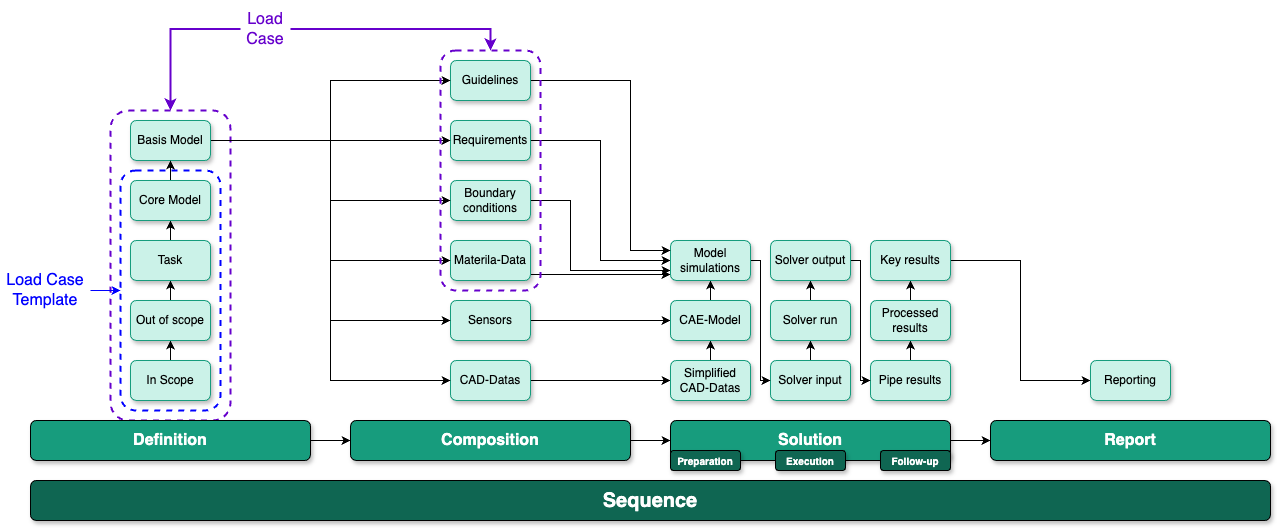
\includegraphics[width=\textwidth]{images/Concept-cae-process.drawio.png}
    \caption{\label{fig:cea-proc}  The CAE core process, illustrated with the stages of a general problem-solving scheme. [ ]}
\end{figure}

Based on the elements and steps involved in this process, a simulation ontology will be created. This will enable us to capture and formalize the elements involved in the configuration process, as well as the interdependencies between them. Particularly important in the context of this thesis are the elements involved in the “Definition” and “Composition” stages, as these lead to a "CAE-Model". Figure[] shows a UML diagram representing the information extracted from Figure[] and the relationships between them.\\

\begin{figure}[h]
    \centering
    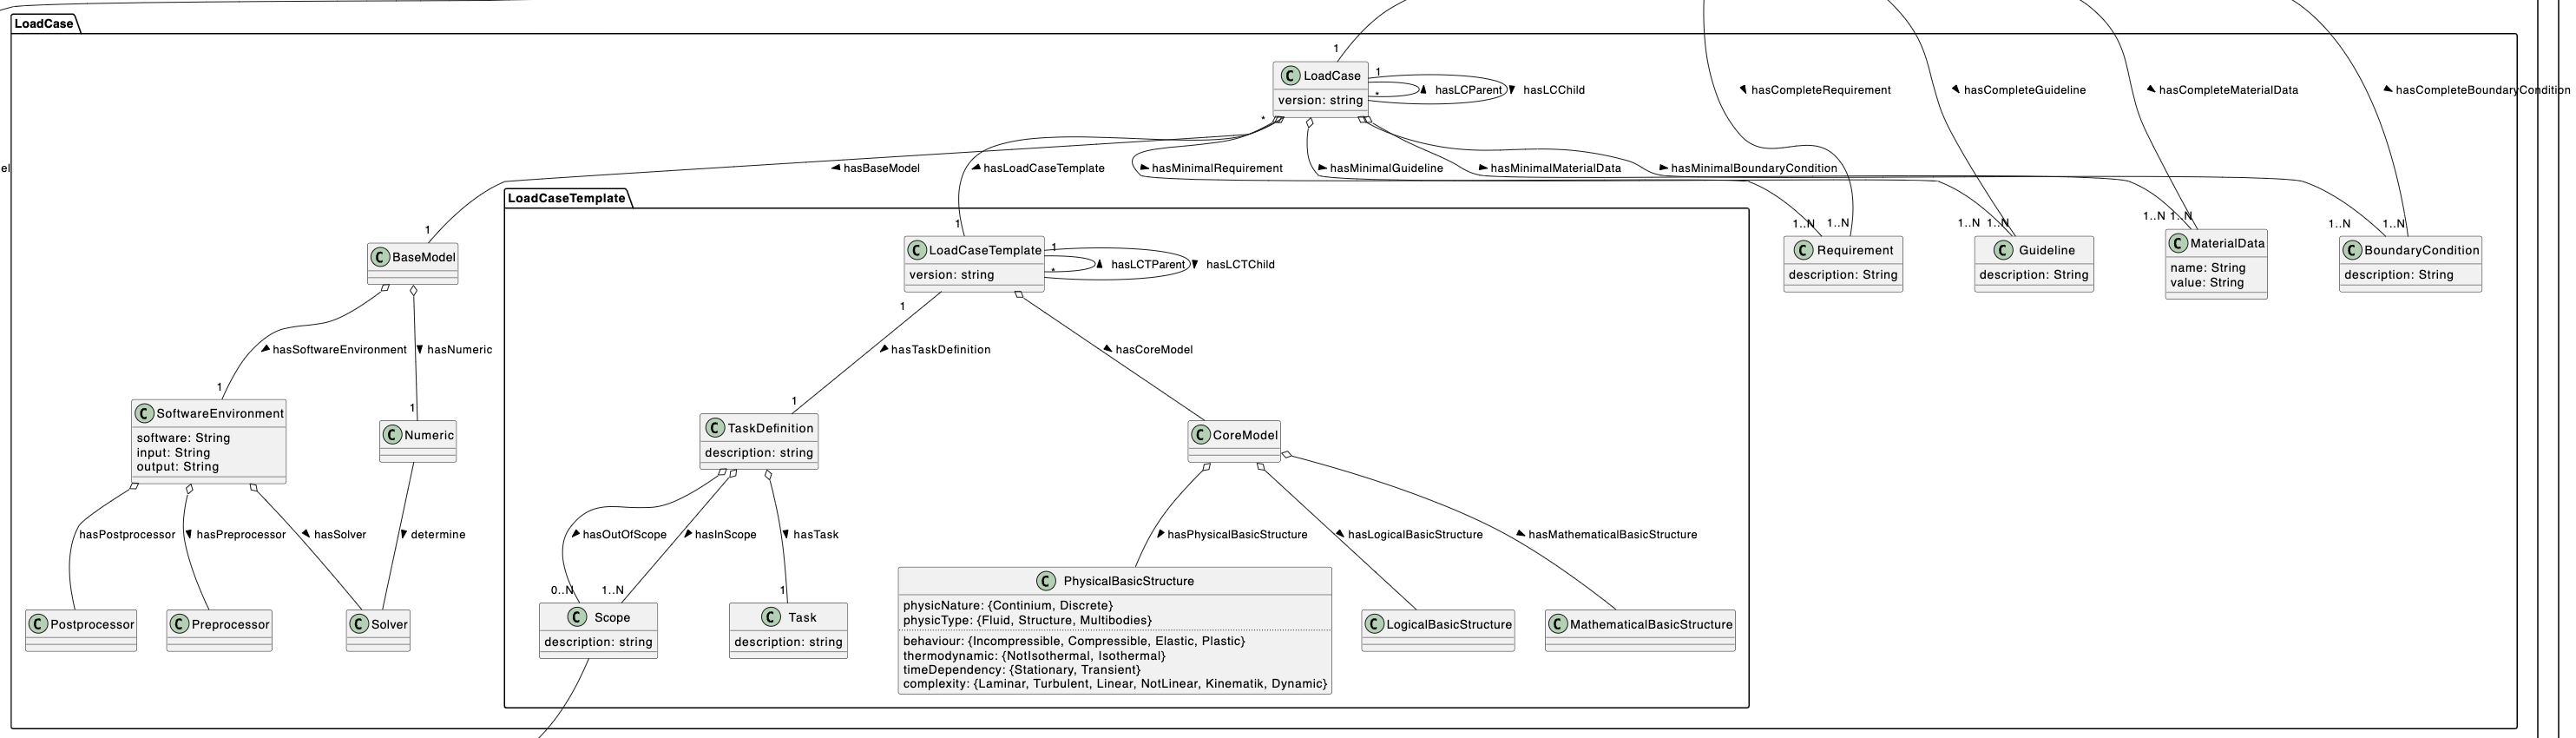
\includegraphics[width=\textwidth]{images/UML-Sim.png}
    \caption{\label{fig:uml-sim}  UML representation of the simulation’s metadata}
\end{figure}


\subsection{Simulation Modeling using Ontology}
There is no single technique for modeling a domain; there are always valid options. The ideal method is almost always determined by the application and extensions you intend to implement. Ontology development is an iterative process. Ontology concepts need to be linked to object (physical or logical) and relationships in your field of interest. These objects are most likely to be nouns (things) or verbs (relations) in the sentences describing your domain. As presented in Section\ref{subsec:sms_analysis}, the researchers behind the “Protégé” software have put together a set of best practices, which will be followed in this work []. The steps to follow are:

\begin{itemize}
    \item Step1: Scope Definition
    \item Step2: Reuse Existing Vocabulary
    \item Step3: Identification of Important Terms
    \item Step4: Class Hierarchy and Taxonomy
    \item Step5: Define Attributes and Properties of Classes — Slots
    \item Step6: Define the Facets of the Slots
    \item Step7: Creation of Instances
\end{itemize}

    \subsubsection{Step1: Scope Definition}
    The development of an ontology begins with the definition of its domain and field of application. To do this, few questions need to be answered []:
    
    \begin{itemize}
        \item What domain will the ontology cover? 
        \item For what purpose will we utilize the ontology? 
        \item To what kinds of queries should the knowledge in the ontology offer answers? 
        \item Who will utilize and maintain the ontology?
    \end{itemize}
    
    The answers to these questions have already been partially addressed in our previous analysis. In this thesis, an ontology will be created to model simulations and their metadata used during configuration. The aim of the ontology is to provide a formalism for the elements involved in the configuration process, and to model the relationships and interdependencies between these elements. Different simulation templates will be stored in the ontology, and information about them can be accessed using SPARQL queries (explained in Section\ref{para:sparql}). This will enable a suitable algorithm to provide assistance to future users. The ontology will be used primarily by simulation engineers. It will be maintained by an expert in semantic technology and expert simulation engineers, who will enrich it with their knowledge.

    
    \subsubsection{Step2: Reuse Existing Vocabulary}
    Setting up an ontology from scratch can be a rather tedious and complex process, requiring a certain level of knowledge in the target domain. That's why it's worth investigating whether there's a similar ontology to the one you want to build, which can be extended and refined to meet your requirements 100\%. Numerous ontologies are available in electronic form on the Internet. Platforms such as \textbf{DBPedia}, \textbf{WikiData} or \textbf{Linked Open Vocabularies (LOV)} allow you to access free ontologies, download them and integrate them into other ontologies.\\
    
    During the study in Chapter\ref{sec:relwork}, a number of simulation ontologies were identified. These include: OSMO [], I2Sim [], OntologySim[] and VIO[]. Unfortunately, given that the elements we want to model (see Figure\ref{fig:cea-proc}) come from conventions defined as part of the EP4.0 project [], it was impossible to find a free ontology that could cover our needs. The ontology will therefore have to be built from scratch, using the structure described in Figure\ref{fig:uml-sim}.


    \subsubsection{Step3: Identification of Important Terms}
    All the important terms can be extracted from the diagram in Figure[]. The most important are:
    \begin{itemize}
        \item LoadCase Template
        \item LoadCase
        \item Basic Model
        \item Core Model
        \item Numeric 
        \item Solver
        \item Physical Basic Structure
        \item Mathematical Basic Structure
        \item Logical Basic Structure
        \item Task
    \end{itemize}

    
    \subsubsection{Step4: Class Hierarchy and Taxonomy}
    There are three main techniques for building a class hierarchy.
    \begin{itemize}
        \item \textbf{A top-down development}: this method begins with the formulation of the most general notions of the domain, followed by the specialization of these concepts.
        \item \textbf{A bottom-up development}: this begins with the definition of the most detailed classes in the hierarchy, then groups these classes into more generic notions.
        \item \textbf{A combination development}: this method combines the two previous approaches. The most important ideas are first identified. They are then generalized and specified as appropriate.
    \end{itemize}
    
    For the purposes of this thesis, the third (hybrid) approach is the most appropriate. Since the majority of key elements have already been defined (top-down), it remains to group those of the same type into more generic notions (bottom-up). The various intermediates elements / classes are presented in the following diagrams:
    
    \begin{figure}
        \centering
            \begin{tikzpicture} 
            \centering
            \umlsimpleclass{Package} 
            \umlsimpleclass[x=-2, y=-2, anchor=north]{LoadCaseTemplate} 
            \umlsimpleclass[x=2, y=-2, anchor=north]{LoadCase} 
            \umlVHVinherit[arm2=-1.2cm]{LoadCaseTemplate}{Package} 
            \umlVHVinherit[arm2=-1.2cm]{LoadCase}{Package} 
            \end{tikzpicture} 
        \caption{\label{fig:distro-art} Classification of “Package”}
    \end{figure}
    
    \begin{figure}
        \centering
            \begin{tikzpicture} 
            \centering
            \umlsimpleclass{Model} 
            \umlsimpleclass[x=-2, y=-2, anchor=north]{BasicModel} 
            \umlsimpleclass[x=2, y=-2, anchor=north]{CoreModel} 
            \umlVHVinherit[arm2=-1.2cm]{BasicModel}{Model} 
            \umlVHVinherit[arm2=-1.2cm]{CoreModel}{Model} 
            \end{tikzpicture} 
        \caption{\label{fig:distro-art} Classification of “Model”}
    \end{figure}
    
    \begin{figure}
        \centering
            \begin{tikzpicture} 
            \centering
            \umlsimpleclass{BasicStructure} 
            \umlsimpleclass[x=-2, y=-2, anchor=north]{PhysicalBasicStructure} 
            \umlsimpleclass[x=4, y=-2, anchor=north]{MathematicalBasicStructure}  
            \umlsimpleclass[x=10, y=-2, anchor=north]{LogicalBasicStructure} 
            \umlVHVinherit[arm2=-1.2cm]{PhysicalBasicStructure}{BasicStructure} 
            \umlVHVinherit[arm2=-1.2cm]{MathematicalBasicStructure}{BasicStructure} 
            \umlVHVinherit[arm2=-1.2cm]{LogicalBasicStructure}{BasicStructure} 
            \end{tikzpicture} 
        \caption{\label{fig:distro-art} Classification of “BasicStructure”}
    \end{figure}
    

    
    \subsubsection{Step5: Define Attributes and Properties of Classes — Slots}
    In order to achieve a complete, connected knowledge model, the properties of the various classes and the relationships between these classes still need to be explicitly defined. Here again, our UML diagram in Figure\ref{fig:uml-sim} comes into play. It contains the definition of each class and their properties.
    
    
    \subsubsection{Step6: Define the Facets of the Slots}
    Slots can have many facets that describe the type of value, the permitted values, the number of values (cardinality) and other characteristics of the values the slot can accept. A facet can be a string, a number, a Boolean literal or an instance of a class. The “range” represents the classes authorized for the value of a property. And the “domain” represents the classes that a property can describe. The diagram in Figure\ref{fig:uml-sim} also shows the relationships between the various classes, as well as their cardinalities.
    
    
    \subsubsection{Step7: Creation of Instances}
    For our purposes, instances will be created using a migration system when our server is first launched (see Chapter\ref{sec:implementation}).
    

\subsection{Case-Based reasoning \label{subsec:cbr}}
Case-based reasoning (CBR) is an approach to building intelligent systems that models the way humans think. Figure\ref{fig:simple-cbr} shows a simplified model of CBR. This method involves recording past experiences in the form of cases. These cases are then retrieved and reused (partially, fully or modified) to solve new problems. The new experience acquired in this way will in turn be stored in the memory and will later help in the resolution of a new case. It's therefore a cycle following a number of stages. Figure\ref{fig:cbr-cycle} shows the CBR cycle. And the stages making up this cycle are as follows.
    
    \begin{enumerate}
        \item Retrieve
        \item Reuse
        \item Revise
        \item Retain
    \end{enumerate}
    
    \begin{figure}[h]
    \centering
    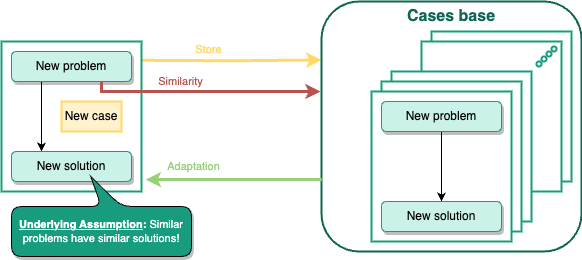
\includegraphics[width=\textwidth]{images/Concept-simplified-cbr-Simplified CBR princip.drawio.png}
    \caption{\label{fig:simple-cbr}  Simplified model of CBR []}
    \end{figure}
    
    \begin{figure}[h]
    \centering
    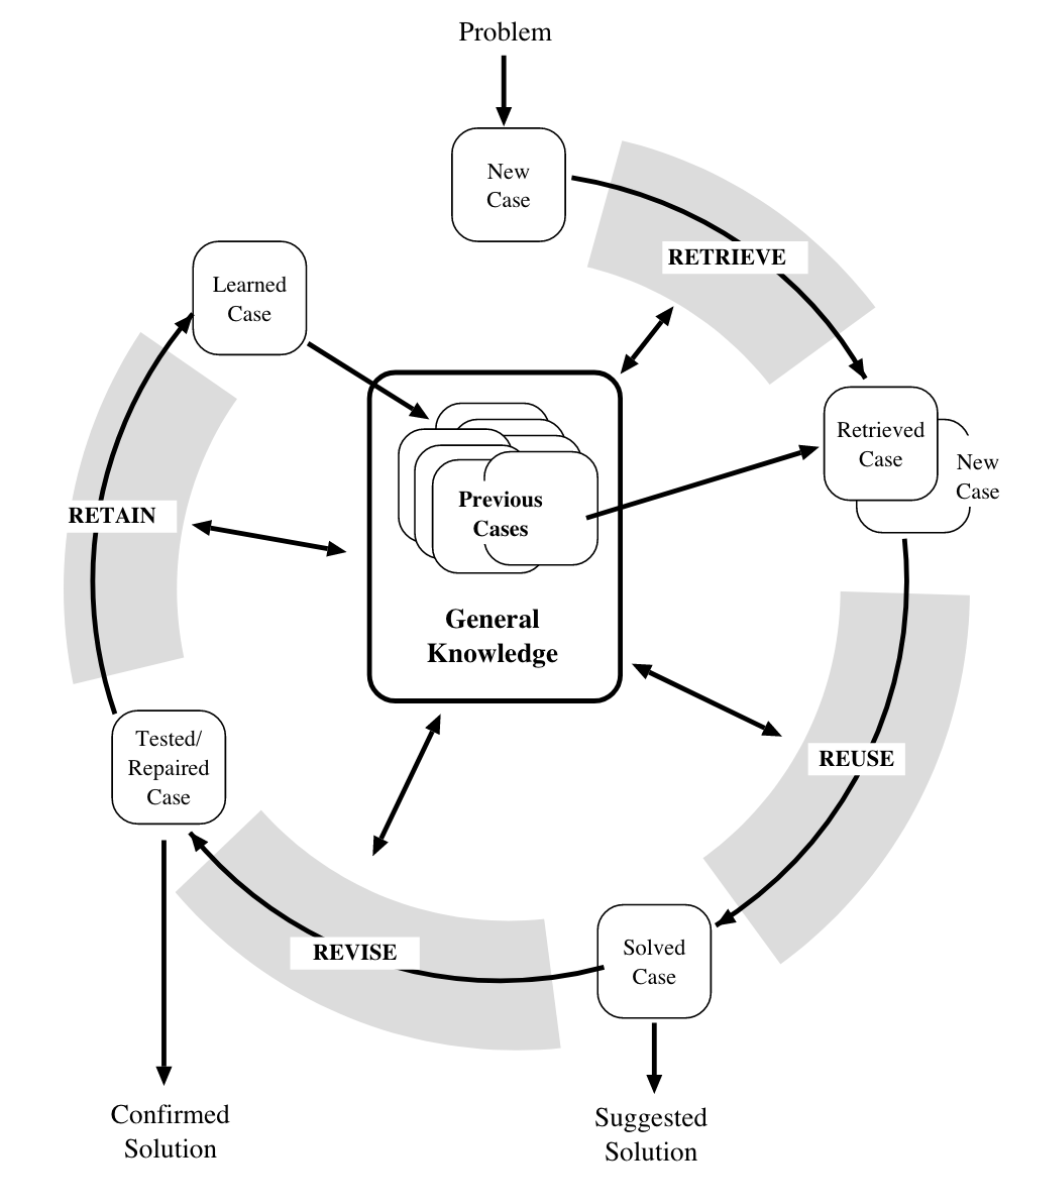
\includegraphics[scale=0.6]{images/Concept-cbr-cycle.png}
    \caption{\label{fig:cbr-cycle}  CBR cycle []}
    \end{figure}
    

    \subsection{Retrieve}
    The aim here is to find the case(s) in the database most similar to the query, taking into account certain similarity functions or criteria. The key question here is how to measure similarity between 2 entities. This will be studied in greater depth in Section\ref{parag:similarity}. The problem that can quickly arise here is that, over time, as the database of cases increases, the efficiency of the search decreases. This is because numerous cases have to be examined to find the most similar ones. There is therefore a sub-field of CBR research which focuses on methods to improve search efficiency. One example is the use of special index structures such as "kd-trees", case-finding networks or discrimination networks [ ].
    
    \subsection{Reuse}
    Once similar cases have been obtained, the answer (or any other information relating to the solution of the problem) from these cases is used to deal with the current problem. There are two types of reuse: simple reuse and reuse with adaptation. 
    
    \begin{itemize}
        \item \textbf{Simple reuse} involves using the recovered answer as a suggested solution for the new problem, without modification. This method is much better suited to classification work, which involves a few solutions but many cases.  For this scenario, all potential solutions are already present in the case base, so adaptation is generally not necessary. 
        
        \item \textbf{Reuse with adaptation} is necessary for synthetic tasks such as planning or configuration. For these tasks, the number of possible solutions far exceeds the number of available examples (or is even infinite).
    \end{itemize}

    Numerous adaptation proposals have been put forward within the CBR framework. The main difference between all these adaptation methods is whether they are transformational or generative.
    
    \begin{itemize}
        \item Transformational adaptation is based on a set of adaptation rules or operators, which specify how variations in the problem lead to the necessary changes in the solution.  
        
        \item Generative adaptation requires the use of a generative problem solver such as LLM. The latter must be able to solve problems based on general knowledge. Here, it's not the case solutions that are really used, but the path (reasoning) taken to obtain these solutions. 
    \end{itemize}

    Adaptation can be a tedious process. This is why the majority of work in the field of CBR seeks to avoid or reduce the modifications to be made once an interesting case has been obtained.


    \subsection{Revise}
    This stage provides feedback on the solution. The aim is to determine whether the solution works and is relevant, through verification in simulations or in the real world. This feedback can take the form of an accuracy score.
    
    
    \subsection{Retain}
    This phase represents the learning phase of the CBR system. In a CBR system, learning consists in adding a new case, generally by modifying a case already in the case base. This new case then becomes available for use in future problem-solving processes.\\
    However, as mentioned above, the constant expansion of the case base can at some point create a utility problem, as it reduces the efficiency of the search. Researchers have devised special algorithms for learning similarity measures. Early techniques focused on the use of feature weights [ ]. But more recent methods tackle the more difficult task of using local and global similarity functions [ ]. 

    
    
    \subsection{Similarity\label{subsec:similarity}}
    As presented in the retrieve step, the main concept of CBR is similarity. This is due to the fact that the cases chosen during the process are those most similar to the current situation (query). Similarity can be formalized by a function $sim: P \times P \rightarrow [0, 1]$, which compares two problem descriptions of type \textbf{P} and returns a score between 0 and 1. The higher this score, the more similar the two problems are considered to be [ ].\\
    For a new problem \textbf{p}, a case $c_1 = (p_1, s_1)$ is more appropriate than a case $c_2 = (p_2, s_2)$ (represented by $c_1 \succ_p c_2$) \textbf{iff} $sim(p, p_2) < sim(p, p_3)$. Here, the exact value of the similarities is not the most important factor, but the fact that these values allow us to give an order of relevance between the different cases considered. This order of preference corresponds to the evaluation of the usefulness of these cases for the treatment of problem \textbf{p} during the reuse phase.\\
    
    The local-global approach, first introduced by Richter [ , ], is the most widely implemented. Figure\ref{fig:cbr-exam} shows an example of similarity calculation using this principle. Here, cases are represented by graphs, in which each \textbf{Node} has attributes $A_i$ of different types $T_i$. For each Node, a local calculation is first performed at the level of these attributes, using a similarity function $_i = sim_{A_i} : T_i \times T_i$ according to the type of attribute. The local similarities are then combined to calculate the global similarity using an appropriate combination. The combination adopted is called the \textbf{amalgamation function: F}, and also takes into account the different weights of the attributes. There are a number of different amalgamation functions:
    \begin{itemize}
        \item \textbf{Weighted Average}: $F(s_1,...,s_n)= \sum_{1=1}^{n} w_i*s_i$
        \item \textbf{Maximum}: $F(s_1,...,s_n) = max\{s_1,...,s_n\}$
        \item \textbf{k-Minimum}: $F(s_1,...,s_n) = s_{ik} \quad with \quad s_{i1} \leq s_{i2} \leq ... \leq s_{in}$
    \end{itemize}
    
    The global similarity can therefore be described mathematically as follows:\\
    \[sim(x,y) = sim((x_1,...,x_n),(y_1,...,y_n)) = F(sim_{A_1}(x_1, y_1),..., sim_{A_n}(x_n, y_n) )\] where \[F: [0,1]_n \rightarrow [0,1]\].\\


    \begin{figure}[h]
    \centering
    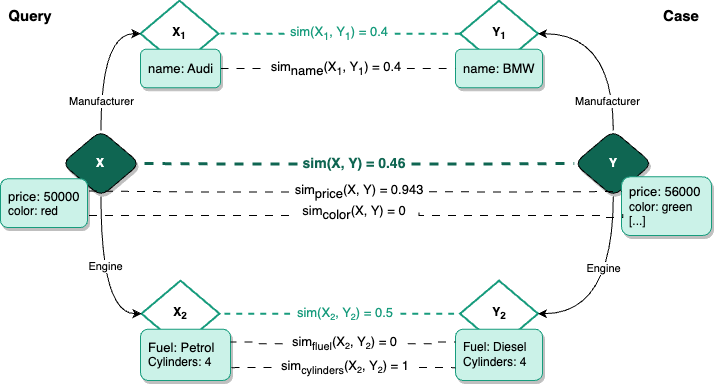
\includegraphics[scale=0.6]{images/Concept-CBR Exemple.drawio.png}
    \caption{\label{fig:cbr-exam}  Calculation of similarity using the local-global principle}
    \end{figure}
    
    \begin{itemize}
        \item $sim_{price}$ is calculated using a \textbf{linear numerical measurement}. The function used is $(n_1, n_2) \rightarrow 1 - abs(n_1 - n_2) / (n_1 + n_2)$. This gives a value of 0.943
        \item for $sim_{color}$ the \textbf{string equality measure} is used. Since \textbf{red != green} the obtained value is 0.
        \item $sim_{fuel}$ is calculated using a string equality measure. Since \textbf{Petrol != Diesel} we obtain a value of 0
        \item $sim_{cylinder}$ is calculated using linear numeric measure. Since they two values are equal, we have a similarity of 1.
        \item $sim(X_2, Y_2)$ is obtained by aggregating the similarities of the Fuel and Cylinders attributes with equal weighting. $sim(X_2, Y_2) = \frac{1}{2} * 0 + \frac{1}{2} * 1 = 0.5$
        \item $sim_{name}$ is calculated using a \textbf{taxonomic similarity measure} based on a semantic taxonomy (Bergmann 2002)[].
        \item $sim(X_1, Y_1) = 1 * 0.4 = 0.4$
        \item finally $sim(X, Y) = \frac{1}{4} sim_{price} + \frac{1}{4} sim_{color} + \frac{1}{4} sim(X_1, Y_1) + \frac{1}{4} sim(X_2, Y_2) = 0.46$

    \end{itemize}


\clearpage
\section{Implementation\label{sec:implementation}}
This chapter describes how the solution concept from Section \ref{subsec:cbr} was realized. This chapter begins by presenting the overall architecture of the solution to be set up. The tools used are then presented. To facilitate understanding of the implementation process, the development strategy is described, followed by the choice of programming languages. For each of these languages, an explanation of their choice is given, followed by a listing of the libraries or packages used. Then the framework's main functions (code snippets) are explained, to give further details on how similarity is calculated. Once the back-end has been explained, a brief presentation of the front-end is given to show how the framework can be used and integrated into applications.


\subsection{Architecture of the Framework \label{subsec:archi-frame}}
Figure\ref{fig:frame-archi} shows the overall structure to be implemented. The chosen architecture is the microservice architecture. Here we have four services:
\begin{itemize}
    \item Client: provides the UI application, which will be used directly by the user
    \item Server: exposes the Reasoning Framework. It exposes an API, which can be consumed to access the functions defined in it. It also features:
    \begin{itemize}
        \item a reasoner: for executing case-based reasoning
        \item a storage layer: to interact with the various storage services
    \end{itemize}
    
    \item a storage service: for non-graphical data
    \item a storage service: for graphical / ontological data
\end{itemize}


\begin{figure}[h]
\centering
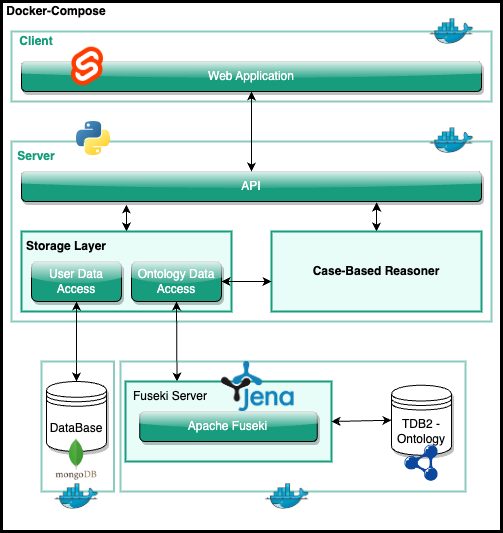
\includegraphics[scale=0.6]{images/SemanticAssistant-Detailled Architecture.drawio.png}
\caption{\label{fig:frame-archi}  Framework architecture}
\end{figure}


\subsection{Used Tools}
    \subsubsection{Protégé}
    Protégé is an ontology development and knowledge management tool that plays a central role in our feasibility study on the use of semantic technologies to support configuration processes in systems engineering. In particular, Protégé facilitates the creation, modification and visualization of ontologies and enables us to define and organize the key attributes relevant for simulations in the automotive industry.
    
    \subsubsection{Apache Jana}
    Apache Jena is a semantic web framework that proves to be very helpful in implementing semantic technologies in our platform. As part of our solution, Apache Jena supports processing RDF data, performing semantic reasoning and executing SPARQL queries to improve the identification of similarities between new and existing simulations in our knowledge graph.
    
    \subsubsection{Apache Fuseki}
    Apache Fuseki is an important component for managing and exposing RDF data as linked data resources. In our study, Apache Fuseki is used to provide an endpoint for querying and retrieving information from the knowledge graph and to ensure seamless integration with other tools and components of our platform.

    
    \subsubsection{TDB2}
    TDB2, the native triple store for Apache Jena, is used for persistent storage of RDF data. This ensures efficient data retrieval and management and contributes to the robustness and scalability of our simulation configuration solution.
    
    
    \subsubsection{MongoDB}
    MongoDB is used as a NoSQL database to store additional non-semantic data related to simulations. It complements the semantic aspects by providing a flexible and scalable storage solution for various parameters and attributes related to simulations in the automotive industry.
    
    \subsubsection{Docker}
    Docker is essential for containerizing our platform by creating an isolated and uniform environment for component deployment and execution. This simplifies deployment, scalability, and repeatability across many computer settings.
    
    \subsubsection{Docker Compose}
    Docker Compose is a tool for managing several Docker containers. It allows for the orchestration of various services inside our platform, ensuring that the many components involved in automotive simulation configuration procedures communicate and interact seamlessly. This improves the overall efficiency and reliability of our solution.

    
\subsection{Development Strategy}
Development begins with the creation of the ontology. Once the ontology had been created, all the architecture elements presented in Section\ref{subsec:archi-frame} were parameterized. These are the Front-end, the Back-end, MongoDB and Apache Fuseki. DockerFiles for setting up the containers were then created. Then a Docker-Compose file was defined for orchestration and communication between containers.\\

Once the setup had been done, a set of functions (CRUD) for manipulating the databases were defined in the back-end. The CBR principles presented in Section\ref{subsec:cbr} were then implemented. This enabled us to:
\begin{itemize}
    \item retrieve cases from the TDB2 database
    \item generate questions for users based on the elements present in the ontology
    \item calculate the similarity between two cases
    \item find the set of cases similar to a problem
\end{itemize}

Once these functions had been fully defined, an API was defined so that they could be accessed and used by other applications.

After completing the back-end implementation, a prototype user interface was coded and integrated with the API.


\subsection{Development of the Ontology}
Two options were considered for ontology development. The first was OntoUML, and the second was Protégé. In this section, we will analyze the strengths and weaknesses of each of these tools, and explain why Protégé was chosen.

    \subsubsection{Usage of OntoUML}
    OntoUML (Ontology Unified Modelling Language) is a language designed primarily for the creation of ontologies. It is based on the Unified Modeling Language (UML), with which software developers and modelers are already familiar. OntoUML relies on the Unified Fundamental Ontology (UFO) as its philosophical basis, enabling complex connections and structures to be defined in a precise and semantically rich way, thus ensuring the consistency and clarity of the final ontology.
    
    \paragraph{Advantages}
        \begin{itemize}
            \item \textbf{Intuitive}: OntoUML builds on the established foundation of UML, providing a familiar, user-friendly experience for those familiar with UML diagrams.
            \item \textbf{Formalism}: Based on UFO, OntoUML offers a rigorous, formal framework for knowledge representation, enabling precise, unambiguous descriptions of ideas and their connections.
            \item \textbf{Integration}: Thanks to its UML base, OntoUML interfaces effortlessly with existing software development tools, making it easy to integrate ontology into software applications.
        \end{itemize}
        
    \paragraph{Inconveniences}
        \begin{itemize}
            \item \textbf{Limited tool support}: Although OntoUML is a language, there is no specialized, widely-used ontology editor.
            \item \textbf{Learning Curve}: Mastering OntoUML may require a steep learning curve, especially for those inexperienced with ontological notions and object-oriented modeling.
            \item \textbf{Complexity}: in some cases, the richness of OntoUML can add a complexity that exceeds the needs of the modeling mission.
        \end{itemize}
    
    \subsubsection{Usage of Protégé}
    Protégé is an open-source ontology authoring tool that makes it easy to create, modify and manage ontologies. It supports a variety of ontology languages, including OWL.
    
    \paragraph{Advantages}
    \begin{itemize}
        \item \textbf{User-friendly interface}: Protégé's simple interface makes ontology building easy for ontology experts and professionals alike.
        \item \textbf{Feature-rich}: Protégé's toolbox enables users to create sophisticated and powerful ontologies.
        \item \textbf{Extensibility}: The platform supports the incorporation of plugins, extending its capabilities to meet a wide range of modeling requirements.
        \item \textbf{Community support}: Protégé benefits from a thriving community that provides resources, documentation, and collaboration opportunities.
        \item \textbf{Interoperability}: Protégé supports a variety of ontology languages, enabling the exchange of information with other systems using different forms.
        \item \textbf{Integration}:  Integration with reasoning tools that can detect errors and extract more information from the ontology.
    \end{itemize}
    
    \paragraph{Inconveniences}
    \begin{itemize}
        \item \textbf{Performance limitations}: Large ontologies can cause performance problems in Protégé, reducing application speed and responsiveness.
        \item \textbf{Limited visualizations}: Although Protégé has visualization capabilities, there may be limitations in developing dynamic and interactive visual representations. The representation it provides may be less natural for people used to UML-based techniques such as OntoUML.
    \end{itemize}
    

    \subsubsection{Why Protégé was chosen over OntoUML}
    Protégé was chosen because of its user-friendly interface and widespread use in the ontology development community. The flexibility of the platform and the support of the community were considered essential for the efficient creation and maintenance of the ontology for our feasibility research. In addition, Protégé's interoperability with OWL is consistent with conventional ontology representation standards. The fact that Protégé supports different ontology languages increases the potential for future integration of the ontology developed with other systems.
    
    The graph in Figure\ref{fig:viz-ontology} shows a representation of the ontology developed. It shows the different classes and the relationships between them.
    
    \begin{figure}[p]
         %%%%%%%%%%%%%%%%%%%%%%%%%%%%%%%%%%%%%%%%%%%%%%%%%%%%%%%%%%%%%%%%%%%%
 %        Generated with the experimental alpha version of the TeX exporter of WebVOWL (version 1.1.3) %%% 
 %%%%%%%%%%%%%%%%%%%%%%%%%%%%%%%%%%%%%%%%%%%%%%%%%%%%%%%%%%%%%%%%%%%%

 %   The content can be used as import in other TeX documents. 
 %   Parent document has to use the following packages   
 %   \usepackage{tikz}  
 %   \usepackage{helvet}  
 %   \usetikzlibrary{decorations.markings,decorations.shapes,decorations,arrows,automata,backgrounds,petri,shapes.geometric}  
 %   \usepackage{xcolor}  

 %%%%%%%%%%%%%%% Example Parent Document %%%%%%%%%%%%%%%%%%%%%%%
 %\documentclass{article} 
 %\usepackage{tikz} 
 %\usepackage{helvet} 
 %\usetikzlibrary{decorations.markings,decorations.shapes,decorations,arrows,automata,backgrounds,petri,shapes.geometric} 
 %\usepackage{xcolor} 

 %\begin{document} 
 %\section{Example} 
 %  This is an example. 
 %  \begin{figure} 
 %    \input{<THIS_FILE_NAME>} % << tex file name for the graph 
 %    \caption{A generated graph with TKIZ using alpha version of the TeX exporter of WebVOWL (version 1.1.3) } 
 %  \end{figure} 
 %\end{document} 
 %%%%%%%%%%%%%%%%%%%%%%%%%%%%%%%%%%%%%%%%%%%%%%%%%%%%%%%%%%%%%%%%%%%%

\definecolor{imageBGCOLOR}{HTML}{FFFFFF} 
\definecolor{owlClassColor}{HTML}{AACCFF}
\definecolor{owlObjectPropertyColor}{HTML}{AACCFF}
\definecolor{owlExternalClassColor}{HTML}{AACCFF}
\definecolor{owlDatatypePropertyColor}{HTML}{99CC66}
\definecolor{owlDatatypeColor}{HTML}{FFCC33}
\definecolor{owlThingColor}{HTML}{FFFFFF}
\definecolor{valuesFrom}{HTML}{6699CC}
\definecolor{rdfPropertyColor}{HTML}{CC99CC}
\definecolor{unionColor}{HTML}{6699cc}
\begin{center} 
\resizebox{\linewidth}{!}{
\begin{tikzpicture}[framed]
\clip (-403.03979294983236pt , 597.2174071205975pt ) rectangle (1418.7574536521824pt , -1453.9836880298267pt);
\tikzstyle{dashed}=[dash pattern=on 4pt off 4pt] 
\tikzstyle{dotted}=[dash pattern=on 2pt off 2pt] 
\fontfamily{sans-serif}{\fontsize{12}{12}\selectfont}
 
\tikzset{triangleBlack/.style = {fill=black, draw=black, line width=1pt,scale=0.7,regular polygon, regular polygon sides=3} }
\tikzset{triangleWhite/.style = {fill=white, draw=black, line width=1pt,scale=0.7,regular polygon, regular polygon sides=3} }
\tikzset{triangleBlue/.style  = {fill=valuesFrom, draw=valuesFrom, line width=1pt,scale=0.7,regular polygon, regular polygon sides=3} }
\tikzset{Diamond/.style = {fill=white, draw=black, line width=2pt,scale=1.2,regular polygon, regular polygon sides=4} }
\tikzset{Literal/.style={rectangle,align=center,
font={\fontsize{12pt}{12}\selectfont \sffamily },
black, draw=black, dashed, line width=1pt, fill=owlDatatypeColor, minimum width=80pt,
minimum height = 20pt}}

\tikzset{Datatype/.style={rectangle,align=center,
font={\fontsize{12pt}{12}\selectfont \sffamily },
black, draw=black, line width=1pt, fill=owlDatatypeColor, minimum width=80pt,
minimum height = 20pt}}

\tikzset{owlClass/.style={circle, inner sep=0mm,align=center, 
font={\fontsize{12pt}{12}\selectfont \sffamily },
black, draw=black, line width=1pt, fill=owlClassColor, minimum size=101pt}}

\tikzset{anonymousClass/.style={circle, inner sep=0mm,align=center, 
font={\fontsize{12pt}{12}\selectfont \sffamily },
black, dashed, draw=black, line width=1pt, fill=owlClassColor, minimum size=101pt}}

\tikzset{owlThing/.style={circle, inner sep=0mm,align=center,
font={\fontsize{12pt}{12}\selectfont \sffamily },
black, dashed, draw=black, line width=1pt, fill=owlThingColor, minimum size=62pt}}

\tikzset{owlObjectProperty/.style={rectangle,align=center,
inner sep=0mm,
font={\fontsize{12pt}{12}\selectfont \sffamily },
fill=owlObjectPropertyColor, minimum width=80pt,
minimum height = 25pt}}

\tikzset{rdfProperty/.style={rectangle,align=center,
inner sep=0mm,
font={\fontsize{12pt}{12}\selectfont \sffamily },
fill=rdfPropertyColor, minimum width=80pt,
minimum height = 25pt}}

\tikzset{owlDatatypeProperty/.style={rectangle,align=center,
fill=owlDatatypePropertyColor, minimum width=80pt,
inner sep=0mm,
font={\fontsize{12pt}{12}\selectfont \sffamily },
minimum height = 25pt}}

\tikzset{rdfsSubClassOf/.style={rectangle,align=center,
font={\fontsize{12pt}{12}\selectfont \sffamily },
inner sep=0mm,
fill=imageBGCOLOR, minimum width=80pt,
minimum height = 25pt}}

\tikzset{unionOf/.style={circle, inner sep=0mm,align=center,
font={\fontsize{12pt}{12}\selectfont \sffamily },
black, draw=black, line width=1pt, fill=unionColor, minimum size=25pt}}

\tikzset{disjointWith/.style={circle, inner sep=0mm,align=center,
font={\fontsize{12pt}{12}\selectfont \sffamily },
black, draw=black, line width=1pt, fill=unionColor, minimum size=20pt}}

\tikzset{owlEquivalentClass/.style={circle,align=center,
font={\fontsize{12pt}{12}\selectfont \sffamily },
inner sep=0mm,
black, solid, draw=black, line width=3pt, fill=owlExternalClassColor, minimum size=101pt,
postaction = {draw,line width=1pt, white}}}

\draw [black,line width=2pt, tension=3] plot [smooth] coordinates {(902.2987798847872pt, -180.34888011433011pt) (1000.664063041456pt, -110.31022075523141pt)  (939.1039456624013pt, -214.19233992686026pt)};
\node[triangleBlack, rotate=-226.4379324986707] at (944.0481567382812pt, -209.4827423095703pt)   (marker0) {};
 \node[triangleBlack, rotate=-218.70705033280888] at (906.0565795898438pt, -175.67141723632812pt)   (INV_marker0) {};
 \draw [black,line width=2pt] plot [smooth] coordinates {(560.3248202971527pt, -1203.777924964349pt) (581.9677186799197pt, -1318.389459376423pt)  (603.6106170626867pt, -1433.000993788497pt)};
\node[triangleBlack, rotate=-169.30698282782595] at (602.4463500976562pt, -1426.835693359375pt)   (single_marker1) {};
 \draw [black,line width=2pt] plot [smooth] coordinates {(585.9851344451697pt, -1190.6409425352972pt) (667.1630111163604pt, -1276.1027880179372pt)  (748.3408877875511pt, -1361.564633500577pt)};
\node[triangleBlack, rotate=-136.47209669895497] at (743.6976928710938pt, -1356.6763916015625pt)   (single_marker2) {};
 \draw [black,line width=2pt] plot [smooth] coordinates {(508.4545633661711pt, -1181.9949016677756pt) (419.71540189017804pt, -1241.2800333433704pt)  (330.976240414185pt, -1300.5651650189652pt)};
\node[triangleBlack, rotate=-236.25392002821187] at (336.3327941894531pt, -1296.986572265625pt)   (single_marker3) {};
 \draw [black,line width=2pt] plot [smooth] coordinates {(620.3046061311322pt, -649.5618793084539pt) (589.0629192507387pt, -876.3513147576313pt)  (557.8212323703451pt, -1103.1407502068087pt)};
\node[triangleBlack, rotate=-187.84375689790573] at (558.7576904296875pt, -1096.342529296875pt)   (single_marker4) {};
 \draw [black, dotted ,line width=2pt] plot [smooth] coordinates {(305.38777806162534pt, -871.6634228694224pt) (233.82223549730918pt, -969.3465534548138pt)  (162.25669293299305pt, -1067.0296840402052pt)};
\node[triangleWhite, rotate=-216.22782275612047] at (165.9130859375pt, -1062.0389404296875pt)   (single_marker5) {};
 \draw [black, dotted ,line width=2pt] plot [smooth] coordinates {(500.1597276121157pt, -1148.1552751110546pt) (341.48868237574266pt, -1130.9168823628713pt)  (182.8176371393696pt, -1113.678489614688pt)};
\node[triangleWhite, rotate=83.799849188741] at (188.99072265625pt, -1114.34912109375pt)   (single_marker6) {};
 \draw [black,line width=2pt] plot [smooth] coordinates {(-153.8302594365342pt, -139.77271675135975pt) (-213.9485047026726pt, -61.69899390412324pt)  (-274.066749968811pt, 16.37472894311327pt)};
\node[triangleBlack, rotate=37.59680366535423] at (-270.35992431640625pt, 11.560806274414062pt)   (single_marker7) {};
 \draw [black,line width=2pt] plot [smooth] coordinates {(285.5717160323048pt, -131.52966991783822pt) (206.79558357342324pt, -21.888729561763967pt)  (128.01945111454168pt, 87.75221079431029pt)};
\node[triangleBlack, rotate=35.697035445832725] at (131.5282745361328pt, 82.86862182617188pt)   (single_marker8) {};
 \draw [black,line width=2pt] plot [smooth] coordinates {(678.260462386362pt, -598.4010265410386pt) (838.7622667535156pt, -596.3930818997546pt)  (984.8147799365408pt, -645.8871940882634pt)};
\node[triangleBlack, rotate=-111.14421723936321] at (979.1914672851562pt, -643.7123413085938pt)   (marker9) {};
 \draw [black,line width=2pt, tension=3] plot [smooth] coordinates {(1212.9020245840793pt, 410.1071476754451pt) (1211.4792880104899pt, 278.2967269111869pt)  (1183.061781147008pt, 407.01524346988793pt)};
\node[triangleBlack, rotate=3.82864276258114] at (1183.528076171875pt, 400.09796142578125pt)   (marker10) {};
 \draw [black,line width=2pt, tension=3] plot [smooth] coordinates {(1166.4666080219256pt, 426.1337039448398pt) (1044.1765687597226pt, 472.07962292206105pt)  (1173.723477730408pt, 455.24277198272296pt)};
\node[triangleBlack, rotate=-106.11556471356982] at (1167.37939453125pt, 457.0715026855469pt)   (marker11) {};
 \draw [black, dotted ,line width=2pt] plot [smooth] coordinates {(577.8006155637627pt, -586.6160939267745pt) (440.77272080033265pt, -552.2013407872923pt)  (303.7448260369026pt, -517.78658764781pt)};
\node[triangleWhite, rotate=75.9022646991013] at (310.11395263671875pt, -519.3861694335938pt)   (single_marker12) {};
 \draw [black, dotted ,line width=2pt] plot [smooth] coordinates {(306.1178878754975pt, -223.1086093220136pt) (284.8055476616099pt, -339.1555961096436pt)  (263.49320744772234pt, -455.2025828972737pt)};
\node[triangleWhite, rotate=-190.40665839867168] at (264.7532043457031pt, -448.34173583984375pt)   (single_marker13) {};
 \draw [black, dotted ,line width=2pt] plot [smooth] coordinates {(214.90159341408997pt, -795.8335014978484pt) (180.0420310076604pt, -927.3529539146026pt)  (145.18246860123082pt, -1058.8724063313568pt)};
\node[triangleWhite, rotate=-194.84499899205565] at (146.7509002685547pt, -1052.9549560546875pt)   (single_marker14) {};
 \draw [black,line width=2pt] plot [smooth] coordinates {(345.4561850634702pt, -214.09869595658193pt) (471.2972797983816pt, -385.99326325122706pt)  (597.1383745332931pt, -557.8878305458721pt)};
\node[triangleBlack, rotate=-143.79245786536686] at (593.5532836914062pt, -552.99072265625pt)   (single_marker15) {};
 \draw [black,line width=2pt] plot [smooth] coordinates {(389.2289868836813pt, 304.63132290407543pt) (396.0014459890827pt, 402.11077538873553pt)  (402.7739050944841pt, 499.5902278733956pt)};
\node[triangleBlack, rotate=-3.9740888488974946] at (402.32830810546875pt, 493.1768493652344pt)   (single_marker16) {};
 \draw [black, dotted ,line width=2pt] plot [smooth] coordinates {(870.896683935559pt, -182.44429095161146pt) (814.1293278209178pt, -53.09489080902701pt)  (757.3619717062763pt, 76.25450933355745pt)};
\node[triangleWhite, rotate=23.69516309466522] at (759.9805297851562pt, 70.28800201416016pt)   (single_marker17) {};
 \draw [black, dotted ,line width=2pt] plot [smooth] coordinates {(433.4867664531697pt, 235.9529879035693pt) (561.2804162667824pt, 188.35450076478594pt)  (689.0740660803951pt, 140.75601362600258pt)};
\node[triangleWhite, rotate=-110.4285476355988] at (682.757568359375pt, 143.10867309570312pt)   (single_marker18) {};
 \draw [black,line width=2pt, tension=3] plot [smooth] coordinates {(1207.2369831513463pt, 461.9283120390655pt) (1320.7140569227793pt, 527.4117934024047pt)  (1225.1077052232258pt, 437.83189544593614pt)};
\node[triangleBlack, rotate=-235.5581162907556] at (1230.342529296875pt, 441.42742919921875pt)   (marker19) {};
 \node[triangleBlack, rotate=-231.30715014571666] at (1211.9229736328125pt, 465.6753845214844pt)   (INV_marker19) {};
 \draw [black,line width=2pt] plot [smooth] coordinates {(1077.6767323707447pt, -687.0629572432058pt) (1165.1640583061499pt, -735.7684981918105pt)  (1252.6513842415548pt, -784.4740391404154pt)};
\node[triangleBlack, rotate=-119.10487337407828] at (1247.1796875pt, -781.4279174804688pt)   (single_marker20) {};
 \draw [black,line width=2pt] plot [smooth] coordinates {(529.7632844860893pt, -1200.094970165666pt) (481.58144731288877pt, -1306.1304692221024pt)  (433.3996101396882pt, -1412.165968278539pt)};
\node[triangleBlack, rotate=-204.43646616227278] at (436.2697448730469pt, -1405.849609375pt)   (single_marker21) {};
 \draw [black,line width=2pt, tension=3] plot [smooth] coordinates {(1173.1221179271831pt, 454.60146744655015pt) (1147.8670177449767pt, 583.217435263306pt)  (1201.7050390644454pt, 463.7128130804862pt)};
\node[triangleBlack, rotate=-164.4344491745153] at (1199.967041015625pt, 469.9364013671875pt)   (marker22) {};
 \draw [black,line width=2pt, tension=3] plot [smooth] coordinates {(337.2016030709791pt, 265.9385369209909pt) (270.3350153407938pt, 365.56246465872647pt)  (372.0000725808532pt, 301.84210944198605pt)};
\node[triangleBlack, rotate=-138.00115553902506] at (367.7633361816406pt, 306.53729248046875pt)   (marker23) {};
 \node[triangleBlack, rotate=-130.18722723504808] at (332.6228332519531pt, 269.81597900390625pt)   (INV_marker23) {};
 \draw [black,line width=2pt] plot [smooth] coordinates {(377.3962825184002pt, 203.43355281041747pt) (350.5121751876869pt, 40.403222999770406pt)  (323.62806785697364pt, -122.62710681087665pt)};
\node[triangleBlack, rotate=-189.3639043481923] at (324.6798400878906pt, -116.24906921386719pt)   (single_marker24) {};
 \node[triangleBlack, rotate=-9.363904348192307] at (376.4200439453125pt, 197.51348876953125pt)   (INV_single_marker24) {};
 \draw [black,line width=2pt] plot [smooth] coordinates {(1083.4178058572377pt, -653.8416678900917pt) (1177.9439334832985pt, -638.0300093853582pt)  (1272.4700611093592pt, -622.2183508806247pt)};
\node[triangleBlack, rotate=-80.50404541472629] at (1265.8828125pt, -623.3201904296875pt)   (single_marker25) {};
 \draw [black,line width=2pt] plot [smooth] coordinates {(599.1827011078692pt, -1169.9746750209715pt) (696.7988027786198pt, -1202.9253807813357pt)  (794.4149044493703pt, -1235.8760865417pt)};
\node[triangleBlack, rotate=-108.65225162239754] at (788.6780395507812pt, -1233.9395751953125pt)   (single_marker26) {};
 \draw [black,line width=2pt] plot [smooth] coordinates {(942.2375107112941pt, -225.17734634365956pt) (1033.5005468295394pt, -218.05608760699798pt)  (1124.763582947785pt, -210.9348288703364pt)};
\node[triangleBlack, rotate=-85.53796174463935] at (1118.7010498046875pt, -211.4078826904297pt)   (single_marker27) {};
 \draw [black,line width=2pt] plot [smooth] coordinates {(-173.69395221202586pt, -181.6464018483957pt) (-263.3670831510683pt, -184.22382442667413pt)  (-353.04021409011074pt, -186.8012470049526pt)};
\node[triangleBlack, rotate=-268.35353532678124] at (-346.6225280761719pt, -186.61679077148438pt)   (single_marker28) {};
 \draw [black,line width=2pt] plot [smooth] coordinates {(1221.9041820430425pt, 418.4837165028311pt) (1299.2974422889695pt, 372.16437453583734pt)  (1376.6907025348964pt, 325.8450325688436pt)};
\node[triangleBlack, rotate=-120.9001089914728] at (1371.2071533203125pt, 329.1269226074219pt)   (single_marker29) {};
 \draw [black,line width=2pt] plot [smooth] coordinates {(264.3370589145335pt, -173.78958844202853pt) (96.30755063181883pt, -176.5643311215124pt)  (-71.72195765089583pt, -179.33907380099626pt)};
\node[triangleBlack, rotate=-269.0537854349364] at (-65.61792755126953pt, -179.23828125pt)   (single_marker30) {};
 \draw [black,line width=2pt] plot [smooth] coordinates {(-156.7885107151389pt, -218.12842598673575pt) (-224.65778771353007pt, -293.71368176854276pt)  (-292.52706471192124pt, -369.2989375503497pt)};
\node[triangleBlack, rotate=-221.9214493833223] at (-288.40576171875pt, -364.7091064453125pt)   (single_marker31) {};
 \draw [black,line width=2pt] plot [smooth] coordinates {(656.9014692091589pt, -557.5342218616042pt) (759.3282598805449pt, -414.09191325169115pt)  (861.7550505519308pt, -270.64960464177807pt)};
\node[triangleBlack, rotate=-35.52908995237802] at (857.9683227539062pt, -275.9527282714844pt)   (single_marker32) {};
 \node[triangleBlack, rotate=-215.5288359291804] at (660.38818359375pt, -552.6513061523438pt)   (INV_single_marker32) {};
 \draw [black,line width=2pt] plot [smooth] coordinates {(587.3132168629131pt, -630.7391457226494pt) (481.3964723723052pt, -714.7809858495739pt)  (375.4797278816973pt, -798.8228259764983pt)};
\node[triangleBlack, rotate=-231.56848124675193] at (380.5068359375pt, -794.833984375pt)   (single_marker33) {};
 \draw [black,line width=2pt] plot [smooth] coordinates {(676.24573582011pt, -613.2458347081035pt) (829.7667772661633pt, -657.7740037232004pt)  (982.1290509909377pt, -661.1319550852667pt)};
\node[triangleBlack, rotate=-89.36527140529863] at (975.7022094726562pt, -661.2031860351562pt)   (marker34) {};
 \draw [black,line width=2pt] plot [smooth] coordinates {(600.8983901681595pt, -1143.799638096911pt) (693.7649888381455pt, -1125.4924951482458pt)  (786.6315875081316pt, -1107.1853521995808pt)};
\node[triangleBlack, rotate=-78.84918205268572] at (780.44287109375pt, -1108.4052734375pt)   (single_marker35) {};
 \draw [black,line width=2pt] plot [smooth] coordinates {(579.4240345687923pt, -616.7108604165147pt) (427.6162678826564pt, -672.7873863093625pt)  (275.80850119652047pt, -728.8639122022104pt)};
\node[triangleBlack, rotate=-249.72678242428245] at (282.0629577636719pt, -726.5535278320312pt)   (single_marker36) {};
 \definecolor{Node37_COLOR}{HTML}{3366cc} 
 \node[owlClass ,minimum size=100pt , fill=Node37_COLOR  , text=white] at (736.86658881785pt, 122.95503695645263pt)   (Node37) {Package\\ {\small (external) }};
\definecolor{Node38_COLOR}{HTML}{3366cc} 
 \node[owlClass ,minimum size=100pt , fill=Node38_COLOR  , text=white] at (385.6942437157149pt, 253.75396457311925pt)   (Node38) {LoadCaseTem...\\ {\small (external) }};
\definecolor{Node39_COLOR}{HTML}{3366cc} 
 \node[owlClass ,minimum size=100pt , fill=Node39_COLOR  , text=white] at (550.861385564373pt, -1153.6636215863869pt)   (Node39) {PhysicalBasicS...\\ {\small (external) }};
\definecolor{Node40_COLOR}{HTML}{3366cc} 
 \node[owlClass ,minimum size=100pt , fill=Node40_COLOR  , text=white] at (254.2809886635609pt, -505.3636736457089pt)   (Node40) {Model\\ {\small (external) }};
\definecolor{Node41_COLOR}{HTML}{3366cc} 
 \node[owlClass ,minimum size=100pt , fill=Node41_COLOR  , text=white] at (227.96808282820842pt, -746.5357646898494pt)   (Node41) {MathematicalB...\\ {\small (external) }};
\definecolor{Node42_COLOR}{HTML}{3366cc} 
 \node[owlClass ,minimum size=100pt , fill=Node42_COLOR  , text=white] at (1033.1166694152685pt, -662.2556843297236pt)   (Node42) {Task\\ {\small (external) }};
\node[Literal ,minimum width=53pt  , text=black] at (814.1127052454607pt, -1101.7678957834778pt)   (Node43) {Literal};
\node[Literal ,minimum width=53pt  , text=black] at (315.1765356684126pt, -1311.1206803146788pt)   (Node44) {Literal};
\node[Literal ,minimum width=53pt  , text=black] at (605.6845446116141pt, -1443.983627188065pt)   (Node45) {Literal};
\definecolor{Node46_COLOR}{HTML}{3366cc} 
 \node[owlClass ,minimum size=100pt , fill=Node46_COLOR  , text=white] at (98.2610604871875pt, 129.1700594500505pt)   (Node46) {Numeric\\ {\small (external) }};
\node[Literal ,minimum width=53pt  , text=black] at (758.5283160684359pt, -1372.2896790093791pt)   (Node47) {Literal};
\definecolor{Node48_COLOR}{HTML}{3366cc} 
 \node[owlClass ,minimum size=100pt , fill=Node48_COLOR  , text=white] at (132.11597918711234pt, -1108.1701431393558pt)   (Node48) {BasicStructure\\ {\small (external) }};
\node[Literal ,minimum width=53pt  , text=black] at (821.862381224733pt, -1245.141092166898pt)   (Node49) {Literal};
\definecolor{Node50_COLOR}{HTML}{3366cc} 
 \node[owlClass ,minimum size=100pt , fill=Node50_COLOR  , text=white] at (335.52849180750604pt, -830.522963770272pt)   (Node50) {LogicalBasicSt...\\ {\small (external) }};
\node[Datatype ,minimum width=49pt  , text=black] at (1271.48761055687pt, -794.960456256366pt)   (Node51) {string};
\node[Datatype ,minimum width=49pt  , text=black] at (-302.1743414531089pt, -380.0430019095122pt)   (Node52) {string};
\node[Datatype ,minimum width=49pt  , text=black] at (403.53797139017087pt, 510.58782313478685pt)   (Node53) {string};
\node[Datatype ,minimum width=49pt  , text=black] at (1297.956357902339pt, -617.9551843724711pt)   (Node54) {string};
\node[Datatype ,minimum width=49pt  , text=black] at (-378.53980128258144pt, -187.5341667890441pt)   (Node55) {string};
\node[Datatype ,minimum width=49pt  , text=black] at (1150.2605524357714pt, -208.94529921575133pt)   (Node56) {string};
\node[owlThing ,minimum size=60pt  , text=black] at (1195.3042352774632pt, 434.4036044442819pt)   (Node57) {Thing};
\node[Literal ,minimum width=53pt  , text=black] at (428.4419872951228pt, -1423.0763868781328pt)   (Node58) {Literal};
\node[Datatype ,minimum width=49pt  , text=black] at (1394.2573922182257pt, 315.33148779653874pt)   (Node59) {string};
\node[Datatype ,minimum width=49pt  , text=black] at (-282.377042383764pt, 27.167051039546344pt)   (Node60) {string};
\definecolor{Node61_COLOR}{HTML}{3366cc} 
 \node[owlClass ,minimum size=100pt , fill=Node61_COLOR  , text=white] at (627.2644529371044pt, -599.0390079288757pt)   (Node61) {CoreModel\\ {\small (external) }};
\definecolor{Node62_COLOR}{HTML}{3366cc} 
 \node[owlClass ,minimum size=100pt , fill=Node62_COLOR  , text=white] at (315.33010665965895pt, -172.94751857357844pt)   (Node62) {BasicModel\\ {\small (external) }};
\definecolor{Node63_COLOR}{HTML}{3366cc} 
 \node[owlClass ,minimum size=100pt , fill=Node63_COLOR  , text=white] at (-122.71500539602128pt, -180.18114366944636pt)   (Node63) {Solver\\ {\small (external) }};
\definecolor{Node64_COLOR}{HTML}{3366cc} 
 \node[owlClass ,minimum size=100pt , fill=Node64_COLOR  , text=white] at (891.3920668239854pt, -229.14481857450664pt)   (Node64) {LoadCase\\ {\small (external) }};
\definecolor{property0_COLOR}{HTML}{3366cc} 
 \definecolor{inv_property0_COLOR}{HTML}{3366cc} 
 % Createing Inverse Property 
\node[owlObjectProperty ,minimum width=80pt , fill=inv_property0_COLOR  , text=white] at (1000.664063041456pt, -124.31022075523141pt)   (property0) {hasLCChild\\ {\small (inverse functional) }};
% owlObjectProperty vs owlObjectProperty
% ,minimum width=80pt vs ,minimum width=90pt
% , fill=inv_property0_COLOR  vs , fill=property0_COLOR 
% , text=white vs , text=white
\node[owlObjectProperty ,minimum width=90pt , fill=property0_COLOR  , text=white] at (1000.664063041456pt, -96.31022075523141pt)   (property0) {hasLCParent\\ {\small (functional) }};
\definecolor{property1_COLOR}{HTML}{3366cc} 
 \node[owlDatatypeProperty ,minimum width=73pt , fill=property1_COLOR  , text=white] at (581.9677186799197pt, -1318.389459376423pt)   (property1) {behaviour};
\definecolor{property2_COLOR}{HTML}{3366cc} 
 \node[owlDatatypeProperty ,minimum width=110pt , fill=property2_COLOR  , text=white] at (667.1630111163604pt, -1276.1027880179372pt)   (property2) {timeDependency};
\definecolor{property3_COLOR}{HTML}{3366cc} 
 \node[owlDatatypeProperty ,minimum width=102pt , fill=property3_COLOR  , text=white] at (419.715401890178pt, -1241.2800333433704pt)   (property3) {thermodynamic};
\definecolor{property4_COLOR}{HTML}{3366cc} 
 \node[owlObjectProperty ,minimum width=120pt , fill=property4_COLOR  , text=white] at (589.0629192507387pt, -876.3513147576313pt)   (property4) {hasPhysicalBasicS...};
\node[rdfsSubClassOf ,minimum width=82pt  , text=black] at (233.82223549730918pt, -969.3465534548138pt)   (property5) {Subclass of};
\node[rdfsSubClassOf ,minimum width=82pt  , text=black] at (341.48868237574266pt, -1130.9168823628713pt)   (property6) {Subclass of};
\definecolor{property7_COLOR}{HTML}{3366cc} 
 \node[owlDatatypeProperty ,minimum width=65pt , fill=property7_COLOR  , text=white] at (-213.9485047026726pt, -61.69899390412324pt)   (property7) {software};
\definecolor{property8_COLOR}{HTML}{3366cc} 
 \node[owlObjectProperty ,minimum width=84pt , fill=property8_COLOR  , text=white] at (206.79558357342324pt, -21.888729561763967pt)   (property8) {hasNumeric};
\definecolor{property9_COLOR}{HTML}{3366cc} 
 \node[owlObjectProperty ,minimum width=105pt , fill=property9_COLOR  , text=white] at (838.7622667535156pt, -596.3930818997546pt)   (property9) {hasOutOfScope};
\definecolor{property10_COLOR}{HTML}{3366cc} 
 \node[owlObjectProperty ,minimum width=98pt , fill=property10_COLOR  , text=white] at (1211.4792880104899pt, 278.2967269111869pt)   (property10) {hasCoreModel\\ {\small (functional) }};
\definecolor{property11_COLOR}{HTML}{3366cc} 
 \node[owlObjectProperty ,minimum width=101pt , fill=property11_COLOR  , text=white] at (1044.1765687597226pt, 472.07962292206105pt)   (property11) {hasBasicModel\\ {\small (functional) }};
\node[rdfsSubClassOf ,minimum width=82pt  , text=black] at (440.77272080033265pt, -552.2013407872923pt)   (property12) {Subclass of};
\node[rdfsSubClassOf ,minimum width=82pt  , text=black] at (284.8055476616099pt, -339.1555961096436pt)   (property13) {Subclass of};
\node[rdfsSubClassOf ,minimum width=82pt  , text=black] at (180.04203100766037pt, -927.3529539146026pt)   (property14) {Subclass of};
\definecolor{property15_COLOR}{HTML}{3366cc} 
 \node[owlObjectProperty ,minimum width=117pt , fill=property15_COLOR  , text=white] at (471.2972797983816pt, -385.99326325122706pt)   (property15) {bmHasCoreModel\\ {\small (functional) }};
\definecolor{property16_COLOR}{HTML}{3366cc} 
 \node[owlDatatypeProperty ,minimum width=72pt , fill=property16_COLOR  , text=white] at (396.00144598908264pt, 402.1107753887355pt)   (property16) {lctVersion\\ {\small (functional) }};
\node[rdfsSubClassOf ,minimum width=82pt  , text=black] at (814.1293278209178pt, -53.09489080902701pt)   (property17) {Subclass of};
\node[rdfsSubClassOf ,minimum width=82pt  , text=black] at (561.2804162667825pt, 188.35450076478594pt)   (property18) {Subclass of};
\definecolor{property19_COLOR}{HTML}{3366cc} 
 \definecolor{inv_property19_COLOR}{HTML}{3366cc} 
 % Createing Inverse Property 
\node[owlObjectProperty ,minimum width=80pt , fill=inv_property19_COLOR  , text=white] at (1320.7140569227793pt, 513.4117934024047pt)   (property19) {hasChild\\ {\small (inverse functional) }};
% owlObjectProperty vs owlObjectProperty
% ,minimum width=80pt vs ,minimum width=75pt
% , fill=inv_property19_COLOR  vs , fill=property19_COLOR 
% , text=white vs , text=white
\node[owlObjectProperty ,minimum width=75pt , fill=property19_COLOR  , text=white] at (1320.7140569227793pt, 541.4117934024047pt)   (property19) {hasParent\\ {\small (functional) }};
\definecolor{property20_COLOR}{HTML}{3366cc} 
 \node[owlDatatypeProperty ,minimum width=78pt , fill=property20_COLOR  , text=white] at (1165.1640583061499pt, -735.7684981918105pt)   (property20) {description};
\definecolor{property21_COLOR}{HTML}{3366cc} 
 \node[owlDatatypeProperty ,minimum width=90pt , fill=property21_COLOR  , text=white] at (481.5814473128887pt, -1306.1304692221024pt)   (property21) {physicNature};
\definecolor{property22_COLOR}{HTML}{3366cc} 
 \node[owlObjectProperty ,minimum width=120pt , fill=property22_COLOR  , text=white] at (1147.8670177449767pt, 583.217435263306pt)   (property22) {caemHasBasicModel\\ {\small (functional) }};
\definecolor{property23_COLOR}{HTML}{3366cc} 
 \definecolor{inv_property23_COLOR}{HTML}{3366cc} 
 % Createing Inverse Property 
\node[owlObjectProperty ,minimum width=80pt , fill=inv_property23_COLOR  , text=white] at (270.3350153407938pt, 351.56246465872647pt)   (property23) {hasLCTChild\\ {\small (inverse functional) }};
% owlObjectProperty vs owlObjectProperty
% ,minimum width=80pt vs ,minimum width=97pt
% , fill=inv_property23_COLOR  vs , fill=property23_COLOR 
% , text=white vs , text=white
\node[owlObjectProperty ,minimum width=97pt , fill=property23_COLOR  , text=white] at (270.3350153407938pt, 379.56246465872647pt)   (property23) {hasLCTParent\\ {\small (functional) }};
\definecolor{property24_COLOR}{HTML}{3366cc} 
 \definecolor{inv_property24_COLOR}{HTML}{3366cc} 
 % Createing Inverse Property 
\node[owlObjectProperty ,minimum width=80pt , fill=inv_property24_COLOR  , text=white] at (350.5121751876869pt, 26.403222999770406pt)   (property24) {hasLoadC...\\ {\small (functional, inv...) }};
% owlObjectProperty vs owlObjectProperty
% ,minimum width=80pt vs ,minimum width=120pt
% , fill=inv_property24_COLOR  vs , fill=property24_COLOR 
% , text=white vs , text=white
\node[owlObjectProperty ,minimum width=120pt , fill=property24_COLOR  , text=white] at (350.5121751876869pt, 54.403222999770406pt)   (property24) {lctHasBasicModel\\ {\small (functional, inverse funct...) }};
\definecolor{property25_COLOR}{HTML}{3366cc} 
 \node[owlDatatypeProperty ,minimum width=50pt , fill=property25_COLOR  , text=white] at (1177.9439334832985pt, -638.0300093853582pt)   (property25) {name};
\definecolor{property26_COLOR}{HTML}{3366cc} 
 \node[owlDatatypeProperty ,minimum width=77pt , fill=property26_COLOR  , text=white] at (696.7988027786198pt, -1202.9253807813357pt)   (property26) {complexity};
\definecolor{property27_COLOR}{HTML}{3366cc} 
 \node[owlDatatypeProperty ,minimum width=69pt , fill=property27_COLOR  , text=white] at (1033.5005468295394pt, -218.05608760699798pt)   (property27) {lcVersion\\ {\small (functional) }};
\definecolor{property28_COLOR}{HTML}{3366cc} 
 \node[owlDatatypeProperty ,minimum width=46pt , fill=property28_COLOR  , text=white] at (-263.3670831510683pt, -184.22382442667413pt)   (property28) {input};
\definecolor{property29_COLOR}{HTML}{3366cc} 
 \node[owlDatatypeProperty ,minimum width=62pt , fill=property29_COLOR  , text=white] at (1299.2974422889693pt, 372.16437453583734pt)   (property29) {version\\ {\small (functional) }};
\definecolor{property30_COLOR}{HTML}{3366cc} 
 \node[owlObjectProperty ,minimum width=73pt , fill=property30_COLOR  , text=white] at (96.30755063181883pt, -176.5643311215124pt)   (property30) {hasSolver\\ {\small (functional) }};
\definecolor{property31_COLOR}{HTML}{3366cc} 
 \node[owlDatatypeProperty ,minimum width=53pt , fill=property31_COLOR  , text=white] at (-224.6577877135301pt, -293.7136817685427pt)   (property31) {output};
\definecolor{property32_COLOR}{HTML}{3366cc} 
 \definecolor{inv_property32_COLOR}{HTML}{3366cc} 
 % Createing Inverse Property 
\node[owlObjectProperty ,minimum width=80pt , fill=inv_property32_COLOR  , text=white] at (759.3282598805449pt, -428.09191325169115pt)   (property32) {lcHasCor...\\ {\small (functional, inv...) }};
% owlObjectProperty vs owlObjectProperty
% ,minimum width=80pt vs ,minimum width=120pt
% , fill=inv_property32_COLOR  vs , fill=property32_COLOR 
% , text=white vs , text=white
\node[owlObjectProperty ,minimum width=120pt , fill=property32_COLOR  , text=white] at (759.3282598805449pt, -400.09191325169115pt)   (property32) {hasLoadCase\\ {\small (functional, inverse funct...) }};
\definecolor{property33_COLOR}{HTML}{3366cc} 
 \node[owlObjectProperty ,minimum width=120pt , fill=property33_COLOR  , text=white] at (481.3964723723052pt, -714.7809858495739pt)   (property33) {hasLogicalBasicSt...};
\definecolor{property34_COLOR}{HTML}{3366cc} 
 \node[owlObjectProperty ,minimum width=83pt , fill=property34_COLOR  , text=white] at (829.7667772661633pt, -657.7740037232004pt)   (property34) {hasInScope};
\definecolor{property35_COLOR}{HTML}{3366cc} 
 \node[owlDatatypeProperty ,minimum width=80pt , fill=property35_COLOR  , text=white] at (693.7649888381454pt, -1125.4924951482458pt)   (property35) {physicType};
\definecolor{property36_COLOR}{HTML}{3366cc} 
 \node[owlObjectProperty ,minimum width=120pt , fill=property36_COLOR  , text=white] at (427.6162678826564pt, -672.7873863093625pt)   (property36) {hasMathematicalB...};
\end{tikzpicture}
}
 \end{center}

         \caption{\label{fig:viz-ontology}  Visualization of a Systematic Map as a Bubble Plot (each color represent different years of publication)}
    \end{figure}

    
\subsection{Used Programming Languages}
    \subsubsection{Python}
        \paragraph{Advantages}
        \begin{itemize}
            \item \textbf{Versatility}: Python's versatility allows for seamless integration with various libraries and frameworks, making it suitable for a wide range of applications.
            \item \textbf{Rapid Development}: Python's syntax and extensive libraries enable rapid prototyping and development, crucial for an efficient master thesis project timeline.
            \item \textbf{Community Support}: The large and active Python community provides extensive documentation, support, and a wealth of resources for problem-solving.
            \item \textbf{Interdisciplinary Integration}: Python's popularity in scientific computing, data analysis, and artificial intelligence domains aligns with the interdisciplinary nature of your thesis.
        \end{itemize}
        
        \paragraph{Used Libraries / Package}
        \begin{table}[H]
            \centering
    	    {\rowcolors{2}{teal!10}{white}
    	    \begin{tabular}{ | m{2.5cm} | m{12cm} | }
                \hline
                \rowcolor{teal!30} Libraries / Packages & Description \\
                
                \hline
                FastAPI & A modern, fast web framework for building APIs with automatic OpenAPI and JSON Schema generation.\\

                \hline
                Uvicorn & A production-grade ASGI (Asynchronous Server Gateway Interface) server used to run FastAPI applications, ensuring efficient handling of asynchronous requests.\\

                \hline
                Pydantic & A data validation library used for defining the data schema in FastAPI, enhancing API request and response handling.\\

                \hline
                pip, setuptools, wheel & Essential tools for package management, distribution, and installation in Python.\\

                \hline
                sparqlwrapper & Facilitates SPARQL query execution in Python, essential for querying semantic knowledge graphs.\\

                \hline
                rdflib & A library for working with RDF (Resource Description Framework) data, supporting semantic data representation.\\

                \hline
                openpyxl & A library for reading and writing Excel files, facilitating data exchange with other applications.\\

                \hline
                levenshtein & A library for calculating Levenshtein distance, beneficial for string similarity comparisons.\\

                \hline
                rapidfuzz & Offers efficient fuzzy string matching, valuable for handling variations in input data.\\

                \hline
                pymongo & A Python driver for MongoDB, supporting integration with MongoDB databases\\
                
                \hline
            \end{tabular}}
            \caption{\label{tab:python-libs} Used Python libraries}
        \end{table}
    
    \subsubsection{JavaScript / TypeScript}
        \paragraph{Advantages}
        \begin{itemize}
            \item Front-end Development: JavaScript and TypeScript are fundamental for building interactive and dynamic user interfaces, enhancing the user experience.
            \item Asynchronous Operations: Asynchronous capabilities of JavaScript and TypeScript are crucial for responsive and efficient web applications.
            \item Widespread Adoption: JavaScript is universally supported in web browsers.
            \item TypeScript: TypeScript, a superset of JavaScript, adds optional static typing, enhancing code reliability and maintainability for larger projects.
            \item Ecosystem: The vast ecosystem of JavaScript libraries and frameworks provides flexibility and choice in front-end development.
        \end{itemize}
        
        \paragraph{Used Libraries / Package}
        \begin{table}[h]
            \centering
    	    {\rowcolors{2}{teal!10}{white}
    	    \begin{tabular}{ | m{2.5cm} | m{12cm} | }
                \hline
                \rowcolor{teal!30} Libraries / Packages & Description \\
                
                \hline
                Svelte & A modern JavaScript framework for building user interfaces with a focus on simplicity and performance. \\

                \hline
                SvelteKit & A full-stack framework built on Svelte, facilitating the creation of complex, scalable web applications and enabling the development of both server-side rendered (SSR) and statically generated applications. \\

                \hline
                Axios & A popular HTTP client for making asynchronous requests, crucial for communicating with backend APIs. \\

                \hline
                Tailwind & A utility-first CSS framework that streamlines the styling process and promotes consistency in the user interface.\\

                \hline
            \end{tabular}}
            \caption{\label{tab:js-libs} Used JavaScript libraries}
        \end{table}
        
\subsection{Framework's main Functions and Classes}
\subsubsection{Extract the schema of a graph}
 When the backend server is launched, one of the first functions to be executed is to extract the ontology schema. To do this, the graph is traversed from an input class considered to be the root. The \textbf{create\_schema\_from\_class} function shown in Listing\ref{lst:create-schema} is used recursively. It extracts the attributes (\textbf{Data Properties}) of the class and is then used on each of the classes linked by a relationship to the one being studied (\textbf{Object Properties}).\\

An important point to note is that in an ontology, classes can be subclasses of another (\textbf{rdfs:subClassOf}). When creating the schema for a class, it is therefore important to check whether it has a parent class. If it does, the properties (Data Properties, Object Properties) of its parent should be added to its schema.
The user can also exclude certain classes from the analysis. This is made possible by the \textbf{EXCLUDED\_CLASSES} global variable, which is a list of classes to be ignored.\\

\begin{lstlisting}[language=Python, caption=Function to create the schema of the ontology, label={lst:create-schema}]
def create_schema_from_class(
        self, class_uri: str, depth: int, visited: dict[str, bool]
    ) -> Node:
        visited[class_uri] = True
        node = Node(None, class_uri, depth)

        # Get all DataProperties of the instance
        data_properties = get_class_data_properties(class_uri)
        # Get all DataProperties of the superClass
        super_data_properties = get_super_class_data_properties(class_uri)
        data_properties += super_data_properties

        # Add all data properties to the node
        for property_uri, type_uri, type_list in data_properties:
            property_suffix_uri = extractSuffixURI(Config.BASEPREFIX, property_uri)
            type = type_list if type_list else extractSchemaType(type_uri)
            node.addAttribute(DataObject(property_suffix_uri, None, type, depth))

        # Get all ObjectProperties of the instance
        object_properties = get_class_object_properties(class_uri)
        # Get all ObjectProperties of his super class
        super_object_properties = get_super_class_object_properties(class_uri)
        object_properties += super_object_properties

        # Add edges
        for property_uri, child_class_name_uri in object_properties:
            child_class_name_turtle_uri = extractSuffixURI(
                Config.BASEPREFIX, child_class_name_uri
            )
            if (child_class_name_turtle_uri not in visited) and (
                child_class_name_turtle_uri not in Config.EXCLUDED_CLASSES
            ):
                property_suffix_uri = extractSuffixURI(Config.BASEPREFIX, property_uri)
                node.addEdge(
                    property_suffix_uri,
                    self.create_schema_from_class(
                        child_class_name_turtle_uri, depth + 1, visited
                    ),
                )

        return node
\end{lstlisting}


\subsubsection{Generate the list of questions}
Once the ontology schema has been extracted, it is searched (Depth search) using the recursive function \textbf{collectQuestionsFromClass}. For each attribute of a class, the \textbf{generateQuestion} function is used, and a question is generated based on the type of the attribute.

\subsubsection{Get the similar cases}
Listing\ref{lst:comp-sim} shows the main function of our framework. This function takes as its parameters the problem (target: Node), the list of attributes that must work, and the list of answers already given. To do this, for each graph in our ontology, the mandatory attributes are checked. If the graph respects these attributes, the function presented in Listing\ref{lst:comp-sim-node} is used to calculate the similarity between the target graph and that of the current iteration.\\


\begin{lstlisting}[language=Python, caption=Function to find the similarity between one case and all the cases in the data-base, label={lst:comp-sim}]
def computeSimilarity(
        self, target: Node, mandatories: list[str], responsesStack: dict[str, Any]
    ) -> list[Similarity]:
        similarities = []

        print("-------------Similar", mandatories)
        for graphKey, graph in self.ontology.graphs.items():
            # Check if the graph respect the mandatories
            check = checkValidGraphByMandatories(graph, mandatories, responsesStack)
            if check:
                simi = Similarity(self.computeSimilarityForNode(graph, target), graph)
                similarities.append(simi)

        mean = self.similarityMean(similarities)
        print("-------------Mean", mean)

        similarities = list(filter(lambda x: x.value >= mean, similarities))

        # order by similarity descending
        similarities.sort(key=lambda x: x.value, reverse=True)

        return similarities
\end{lstlisting}
    
    
    
\subsubsection{Get the similar cases} 
Here the principle of local-to-global calculation presented in Section\ref{subsec:similarity} is implemented. First we iterate over the set of Node target attributes and for each pair of values, the function presented in Listing\ref{lst:comp-sim-att} is called. This calculates the similarity value between two attributes according to their type. Then, for each Edge in our graph, the function is used iteratively.
After iterating over all the attributes and edges (child nodes), the similarity value between the two nodes is calculated by applying the same weight to each attribute and child.\\

\begin{lstlisting}[language=Python, caption=Function to find the similarity between one case and all the cases in the data-base, label={lst:comp-sim-node}]
def computeSimilarityForNode(self, node: Node, target: Node) -> float:
        # Local computation
        attributSimilarity = 0
        numberOfAttribute = 0
        for key, targetAttribute in target.attributes.items():
            if targetAttribute.value is not None:
                nodeAttribute = node.getAttribute(key)

                if nodeAttribute is None:
                    continue

                sim = self.computeSimilarityForAttribute(nodeAttribute, targetAttribute)
                attributSimilarity += sim
                numberOfAttribute += 1

        # Global computation
        childSimilarity = 0
        numberOfEdges = 0
        for key, targetEdges in target.edges.items():
            nodeEdges = node.getEdge(key)

            if nodeEdges is None:
                continue

            # iterate over all the edeges of this node with the same URI
            collectorSim = [0]
            for targetEdge in targetEdges:
                for nodeEdge in nodeEdges:
                    if nodeEdge is not None:
                        collectorSim.append(
                            self.computeSimilarityForNode(
                                nodeEdge["childNode"], targetEdge["childNode"]
                            )
                        )

            sim = max(collectorSim)
            childSimilarity += sim
            numberOfEdges += 1

        if (numberOfAttribute + numberOfEdges) == 0:
            return 0

        nodeSimilarity = (attributSimilarity + childSimilarity) / (
            numberOfAttribute + numberOfEdges
        )

        return nodeSimilarity
\end{lstlisting}



\subsubsection{Find the similarity value between two attributes} 
Calculating the similarity between two attributes depends largely on their type. In the function presented in Listing\ref{lst:comp-sim-att}, a distinction is made between cases based on the type of attributes. Depending on the type, a specific utility function is used.\\

\begin{lstlisting}[language=Python, caption=Function to compute the similarity value between two attributes, label={lst:comp-sim-att}]
def computeSimilarityForAttribute(
        self, nodeAttribute: DataObject, targetAttribute: DataObject
    ) -> float:
        similarity = 0

        match nodeAttribute.type:
            case "string":
                similarity = computeStringLevensteinSimilarity(
                    nodeAttribute.value, targetAttribute.value
                )
            case "int":
                similarity = computeNumericSigmoidSimilarity(
                    nodeAttribute.value, targetAttribute.value
                )
            case "double":
                similarity = computeNumericSigmoidSimilarity(
                    nodeAttribute.value, targetAttribute.value
                )
            case "decimal":
                similarity = computeNumericSigmoidSimilarity(
                    nodeAttribute.value, targetAttribute.value
                )
            case "float":
                similarity = computeNumericSigmoidSimilarity(
                    nodeAttribute.value, targetAttribute.value
                )
            case "boolean":
                similarity = self.computeEqualSimilarity(
                    nodeAttribute.value, targetAttribute.value
                )
            case "date":
                similarity = computeStringSortRatio(
                    nodeAttribute.value, targetAttribute.value
                )
            case _:
                similarity = self.computeEqualSimilarity(
                    nodeAttribute.value, targetAttribute.value
                )

        return similarity
\end{lstlisting}
    

\subsection{Similarity Measures}
For the same type, there are numerous functions for calculating similarity. The choice of one depends on the case and the purpose. In this section, various functions for \textbf{String} and \textbf{Numeric} will be presented, along with the cases in which each of them is appropriate.
    
    \subsubsection{String}
    The function in Listing\ref{lst:leven-string} uses Levenshtein's algorithm to calculate how different two Strings are from each other. It is suitable for long texts or when you want to make a comparison while allowing a certain degree of error.\\
    
\begin{lstlisting}[language=Python, caption=Levenstein distance between two strings, label={lst:leven-string}]
# Compute the Levenstein distance between the two strings
def computeStringLevensteinSimilarity(nodeValue: str, targetValue: str) -> float:
    return fuzz.partial_ratio(nodeValue, targetValue)
\end{lstlisting}
    
    
    The function in Listing\ref{lst:leven-string-ratio} works like the previous function, but ignores special characters such as full stops or commas.\\
    
\begin{lstlisting}[language=Python, caption=Levenstein distance between two strings without considering special characters, label={lst:leven-string-ratio}]
def computeStringSortRatio(nodeValue: str, targetValue: str) -> float:
    return fuzz.token_sort_ratio(nodeValue, targetValue)
\end{lstlisting}





    \subsubsection{Numeric}
    
    \textbf{Exponential similarity} in Listing\ref{lst:expo-sim-num} is useful when you want to emphasize the sensitivity to proximity. It is suitable for cases where small differences between numeric values should result in significantly higher similarity scores.\\
    
\begin{lstlisting}[language=Python, caption=Function to compute the similarity value between two attributes, label={lst:expo-sim-num}]
# Compute the Exponential similarity between two numeric values
def computeNumericExponentialSimilarity(value1, value2):
    num1 = int(value1)
    num2 = int(value2)
    return math.exp(-abs(num1 - num2))
\end{lstlisting}
    
    
    \textbf{Fuzzy similarity} in Listing\ref{lst:fuzzy-sim-num} is beneficial when dealing with uncertain or imprecise numeric data. It can handle situations where the exact values may not be known, and there is a need to capture the degree of similarity despite the fuzziness in the data.\\
\begin{lstlisting}[language=Python, caption=Function to compute the similarity value between two attributes, label={lst:fuzzy-sim-num}]
# Compute the Fuzzy similarity between two numeric values
def computeNumericFuzzySimilarity(value1, value2):
    num1 = int(value1)
    num2 = int(value2)
    return 1 - abs(num1 - num2) / (num1 + num2)
\end{lstlisting}

    
    \textbf{Sigmoid similarity} in Listing\ref{lst:sigmo-sim-num} is appropriate when you expect the similarity to saturate at a certain point, indicating that beyond a specific difference threshold, additional proximity has a diminishing impact.\\

\begin{lstlisting}[language=Python, caption=Function to compute the similarity value between two attributes, label={lst:sigmo-sim-num}]
# Compute the sigmoid similarity between two numeric values
def computeNumericSigmoidSimilarity(value1, value2):
    num1 = int(value1)
    num2 = int(value2)
    return 1 / (1 + math.exp(-(num1 - num2)))
\end{lstlisting}
        
In summary, the choice of similarity computation method depends on the nature of the data and the desired characteristics of the similarity measure. Exponential similarity emphasizes proximity sensitivity, fuzzy similarity accommodates uncertainty, and sigmoid similarity is suitable for situations where similarity saturates with increasing proximity.

\subsection{Web Application}
As already explained in the previous chapters, a prototype UI has been set up in order to demonstrate the use of the CBR mechanism in practical cases. In this section, the different views and elements of this UI will be presented, along with their usefulness.

    \subsubsection{The home page}
    Figure\ref{fig:proto-home} shows the home view of the UI. Here the user can create a new account in which to work or choose an existing account. Each account has a list of configuration processes.
    
    \begin{figure}[h]
    \centering
    \frame{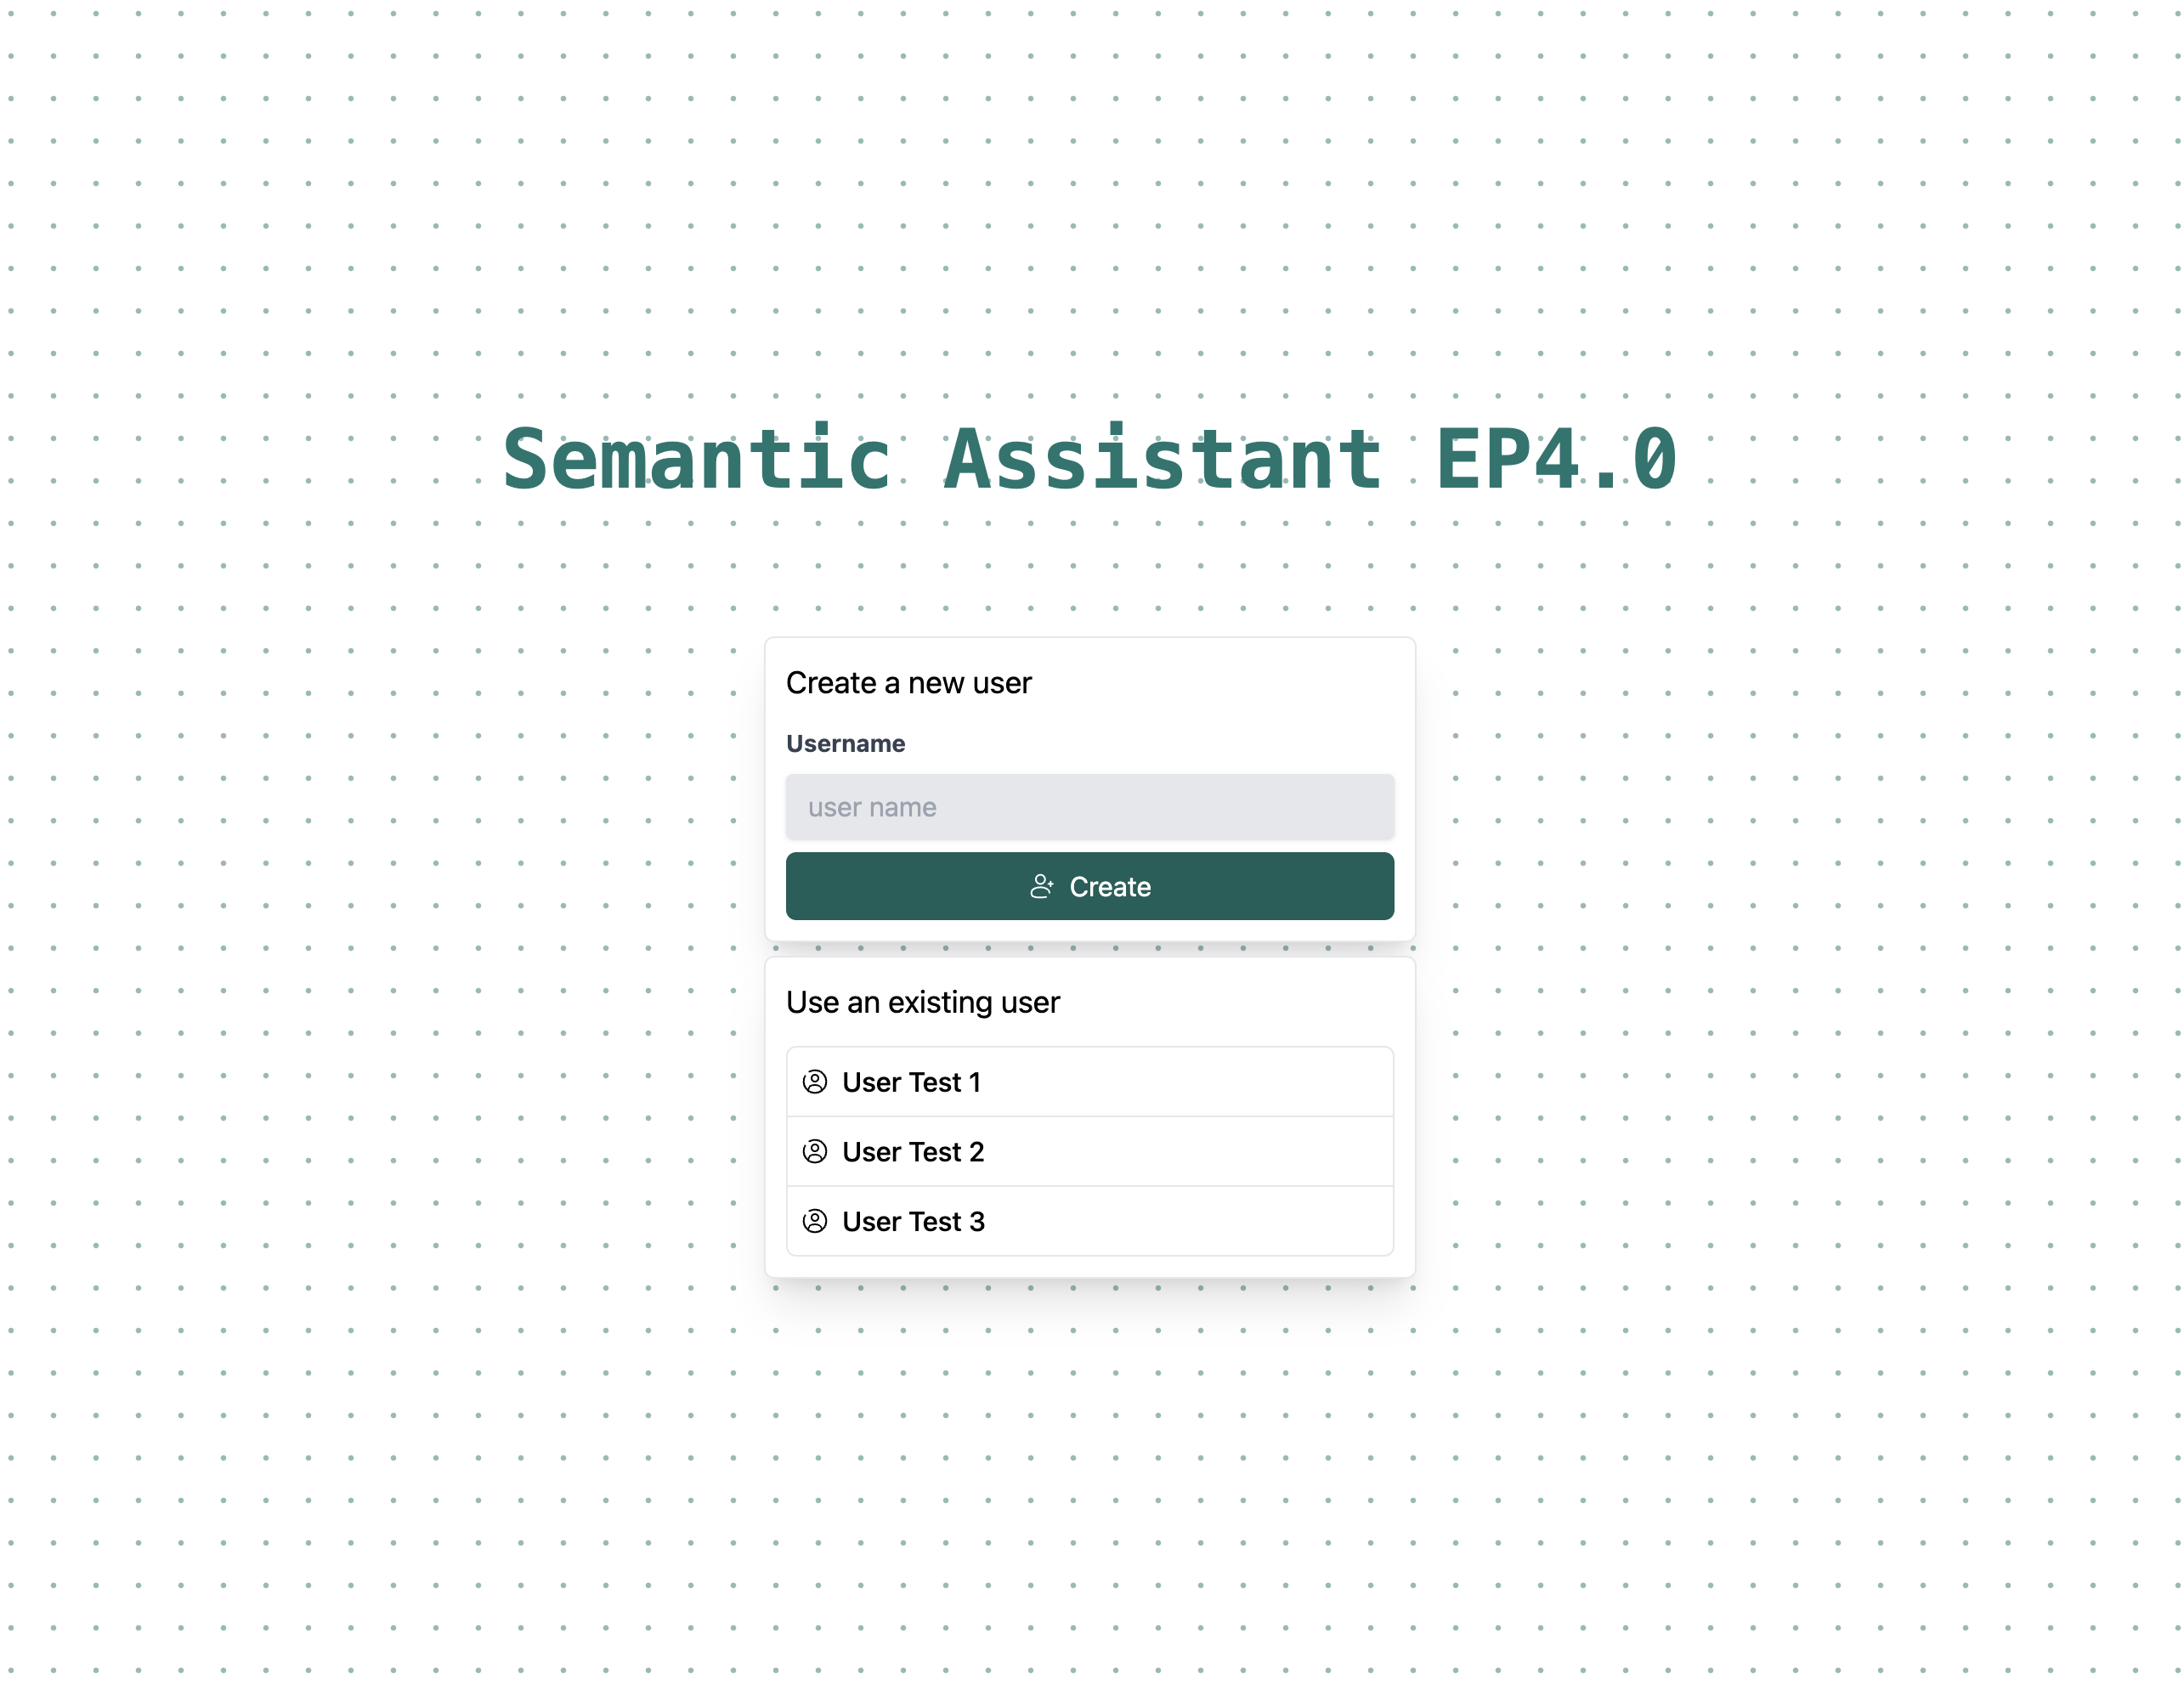
\includegraphics[width=\textwidth]{images/proto-home.png}}
    \caption{\label{fig:proto-home}  Home view of the UI prototype}
    \end{figure}
    
    
    \subsubsection{The working page}
    Figure\ref{fig:proto-demo} shows the working view. This is where all operations are performed. 
    
    \begin{itemize}
        \item The sidebar \textbf{(1)} lists all the processes associated with the current user. It can also be used to create and delete a process.
        \item The box at the bottom left \textbf{(2)} shows the name of the current user and provides a button for logging out and going to the home page (see Figure\ref{fig:proto-home}).
        \item The title bar \textbf{(3)} shows the name of the selected configuration and allows you to modify or delete it.
        \item The buttons at the bottom right \textbf{(4)} are used to manage the zoom percentage of the decision tree shown in the center of the work area.
    \end{itemize}
    
    \begin{figure}[h]
    \centering
    \frame{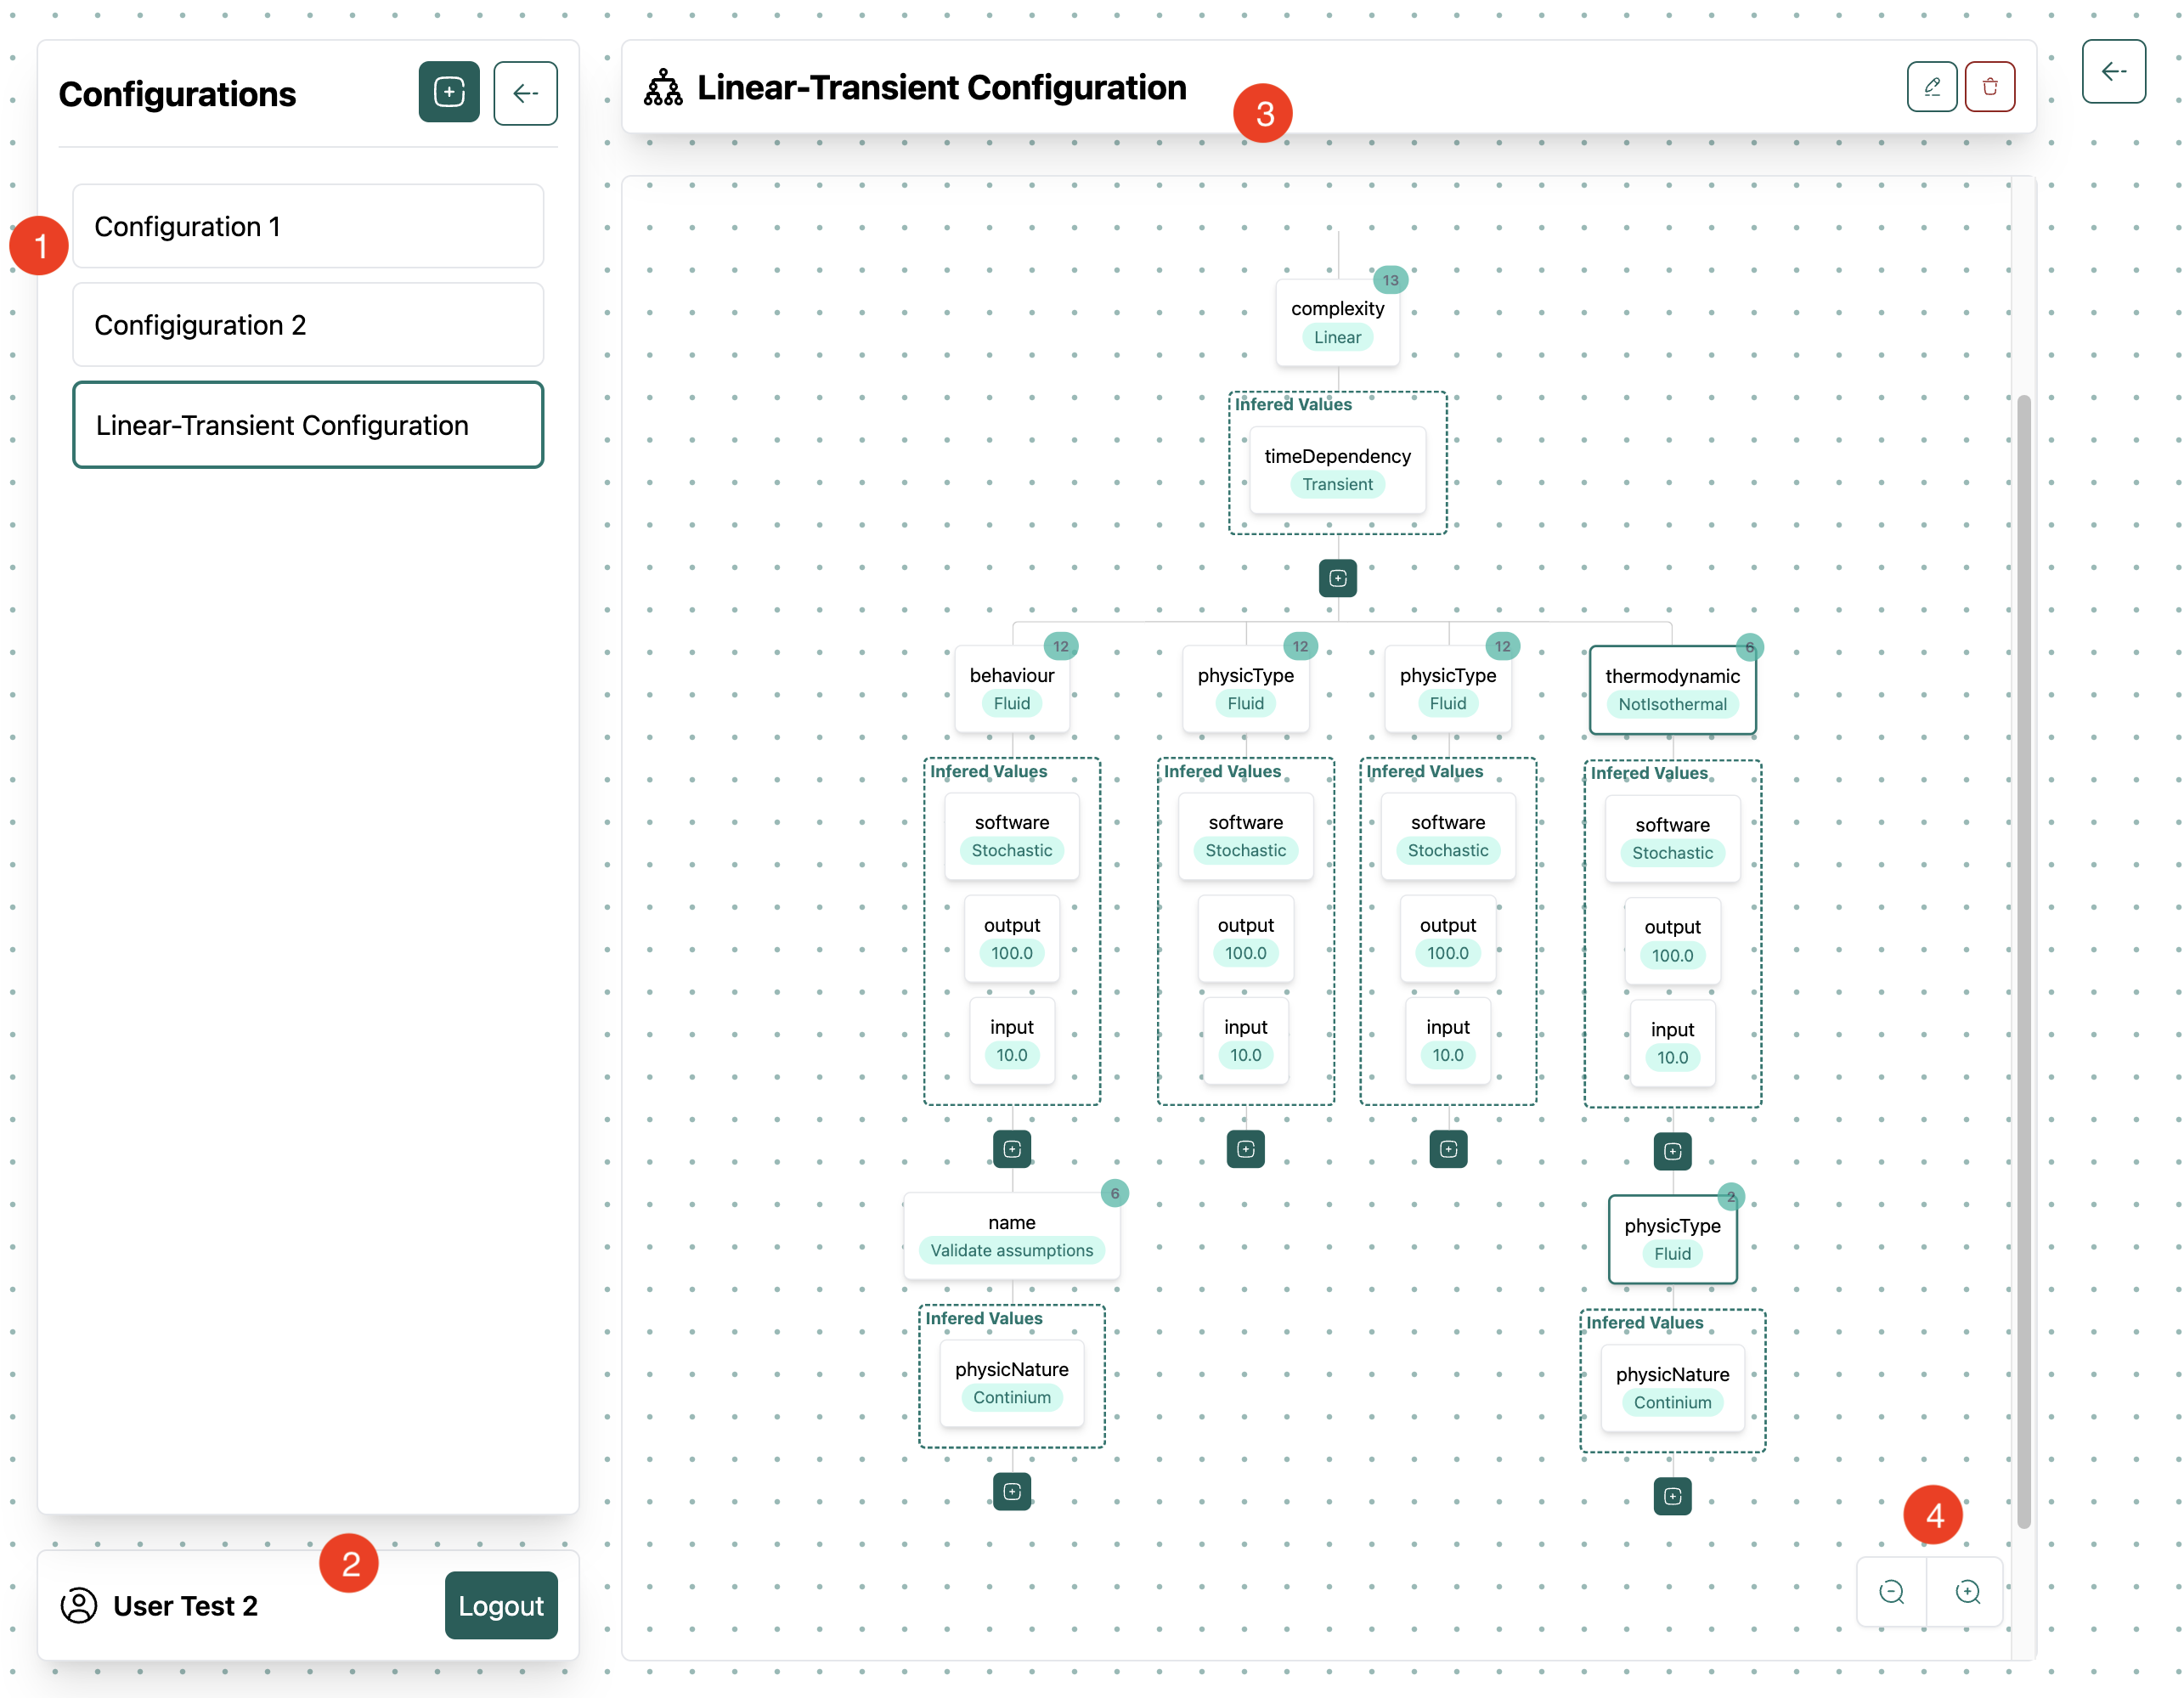
\includegraphics[width=\textwidth]{images/proto-demo.png}}
    \caption{\label{fig:proto-demo}  Main view of the UI prototype}
    \end{figure}
    
    
    \subsubsection{Answering to question}
    To add an answer to the tree, simply click on the “+” button below a Node. Figure\ref{fig:proto-demo-add-answer} shows the dialogue box that appears once you have clicked on this button. This dialogue box contains:
    
    \begin{itemize}
        \item \textbf{(1)} an entry for selecting the element for which you would like to give a value
        \item \textbf{(2)} an entry for giving the value of this element. As shown in Figure\ref{fig:proto-demo-add-answer-proba} a suggestion of possible values is automatically made. And for each of the suggested values, a probability of use is provided, allowing you to find out how many similar simulations have used this value.
        \item a “mandatory” switch \textbf{(3)} to define whether only graphs with exactly the value selected for the element selected should be taken into account
        \item In \textbf{(4)} we have the question asked for this element. This is generated automatically by the backend.
    \end{itemize}
    

    \begin{figure}[h]
        \centering
        \begin{subfigure}[b]{0.45\textwidth}
            \centering
            \frame{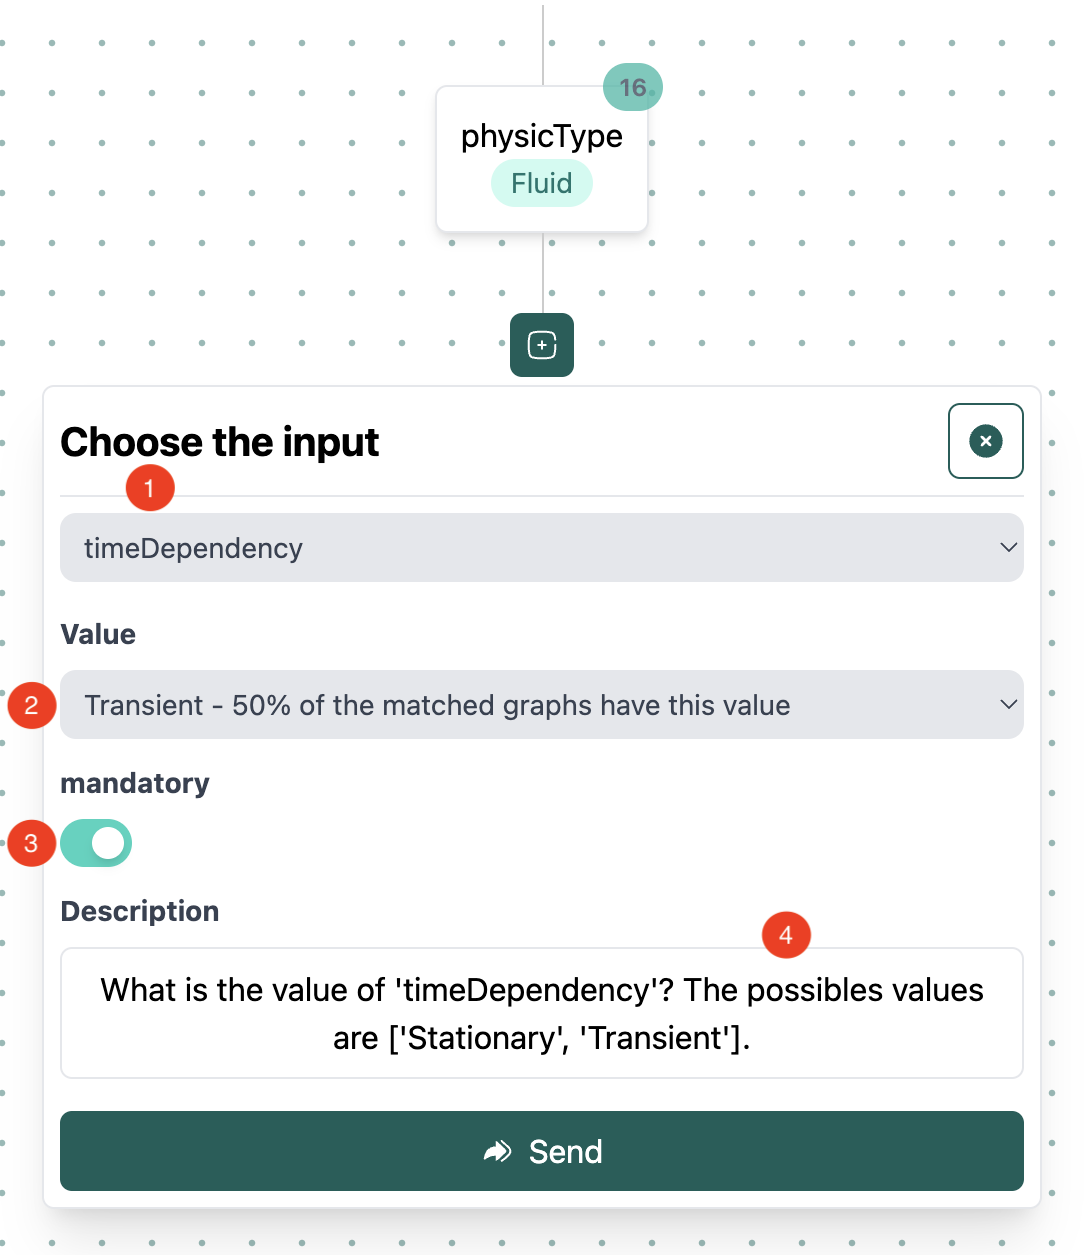
\includegraphics[width=\textwidth]{images/proto-demo-add-answer.png}}
            \caption{\label{fig:proto-demo-add-answer} Dialog to answer to a question}
        \end{subfigure}
        \begin{subfigure}[b]{0.45\textwidth}
            \centering
            \frame{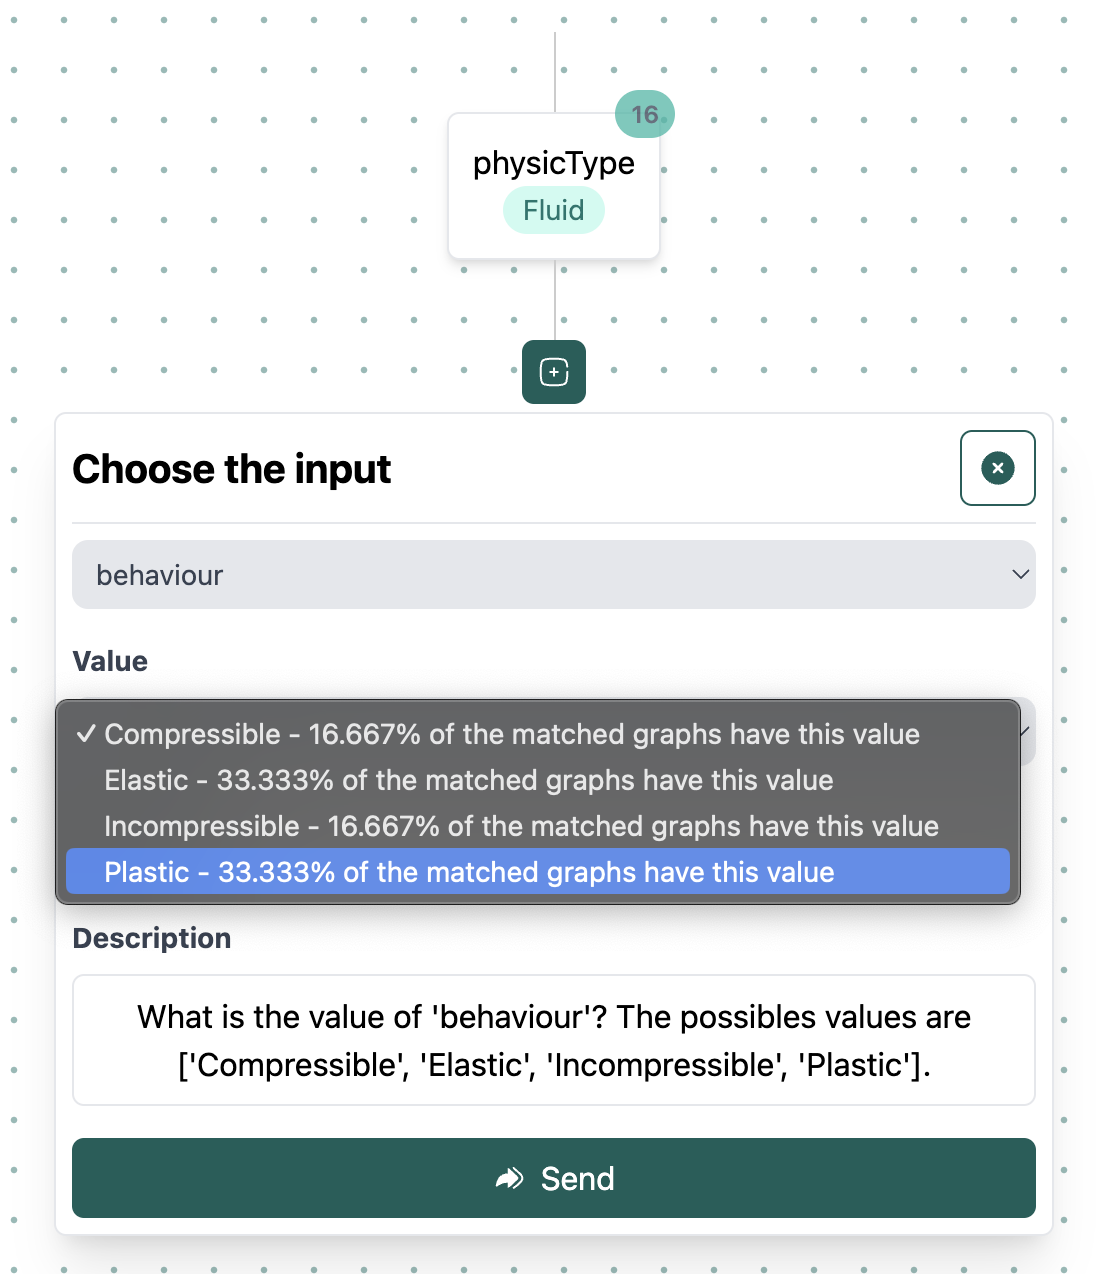
\includegraphics[width=\textwidth]{images/proto-demo-add-answer-proba.png}}
            \caption{\label{fig:proto-demo-add-answer-proba} Probability of usage}
        \end{subfigure}
    \end{figure}
    
    
    \subsubsection{Edit / Delete an answer}
    It is also possible to edit or delete an answer given previously. Figure\ref{fig:proto-demo-edit-delete-answer} shows the elements of our interface which allow this to be done. 
    
    \begin{itemize}
        \item when a Node (response) in the graph is edited, this automatically deletes all the child Nodes it had, since these may no longer be relevant for the new values of the modified Node
        \item when a Node is deleted, its child Nodes are also deleted
    \end{itemize}

    \begin{figure}[h]
    \centering
    \frame{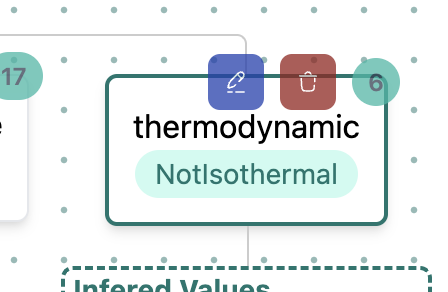
\includegraphics[scale=0.5]{images/proto-demo-edit-delete-answer.png}}
    \caption{\label{fig:proto-demo-edit-delete-answer}  Edit / Delete an answer (a Node)}
    \end{figure}

    
    \subsubsection{Inspecting results}
    After each response, the reasoner recalculates the similar simulations and returns them. You can see the number of simulations found in the top right-hand corner of each Node. For more details, simply click on the Node you wish to inspect. Figure\ref{fig:proto-demo-detail} shows the details of one of these Nodes.
    
    \begin{itemize}
        \item In \textbf{(1)} we have information about the number of simulations found.
        \item The selection list \textbf{(2)} allows you to choose one of the simulations found in order to inspect it.
        \item Once one of the simulations has been chosen, we can see the percentage of similarity \textbf{(3)} of this simulation with the one currently being configured.
        \item The table in \textbf{(4)} shows all the attributes of this simulation and their values.
    \end{itemize}
    
    \begin{figure}[h]
    \centering
    \frame{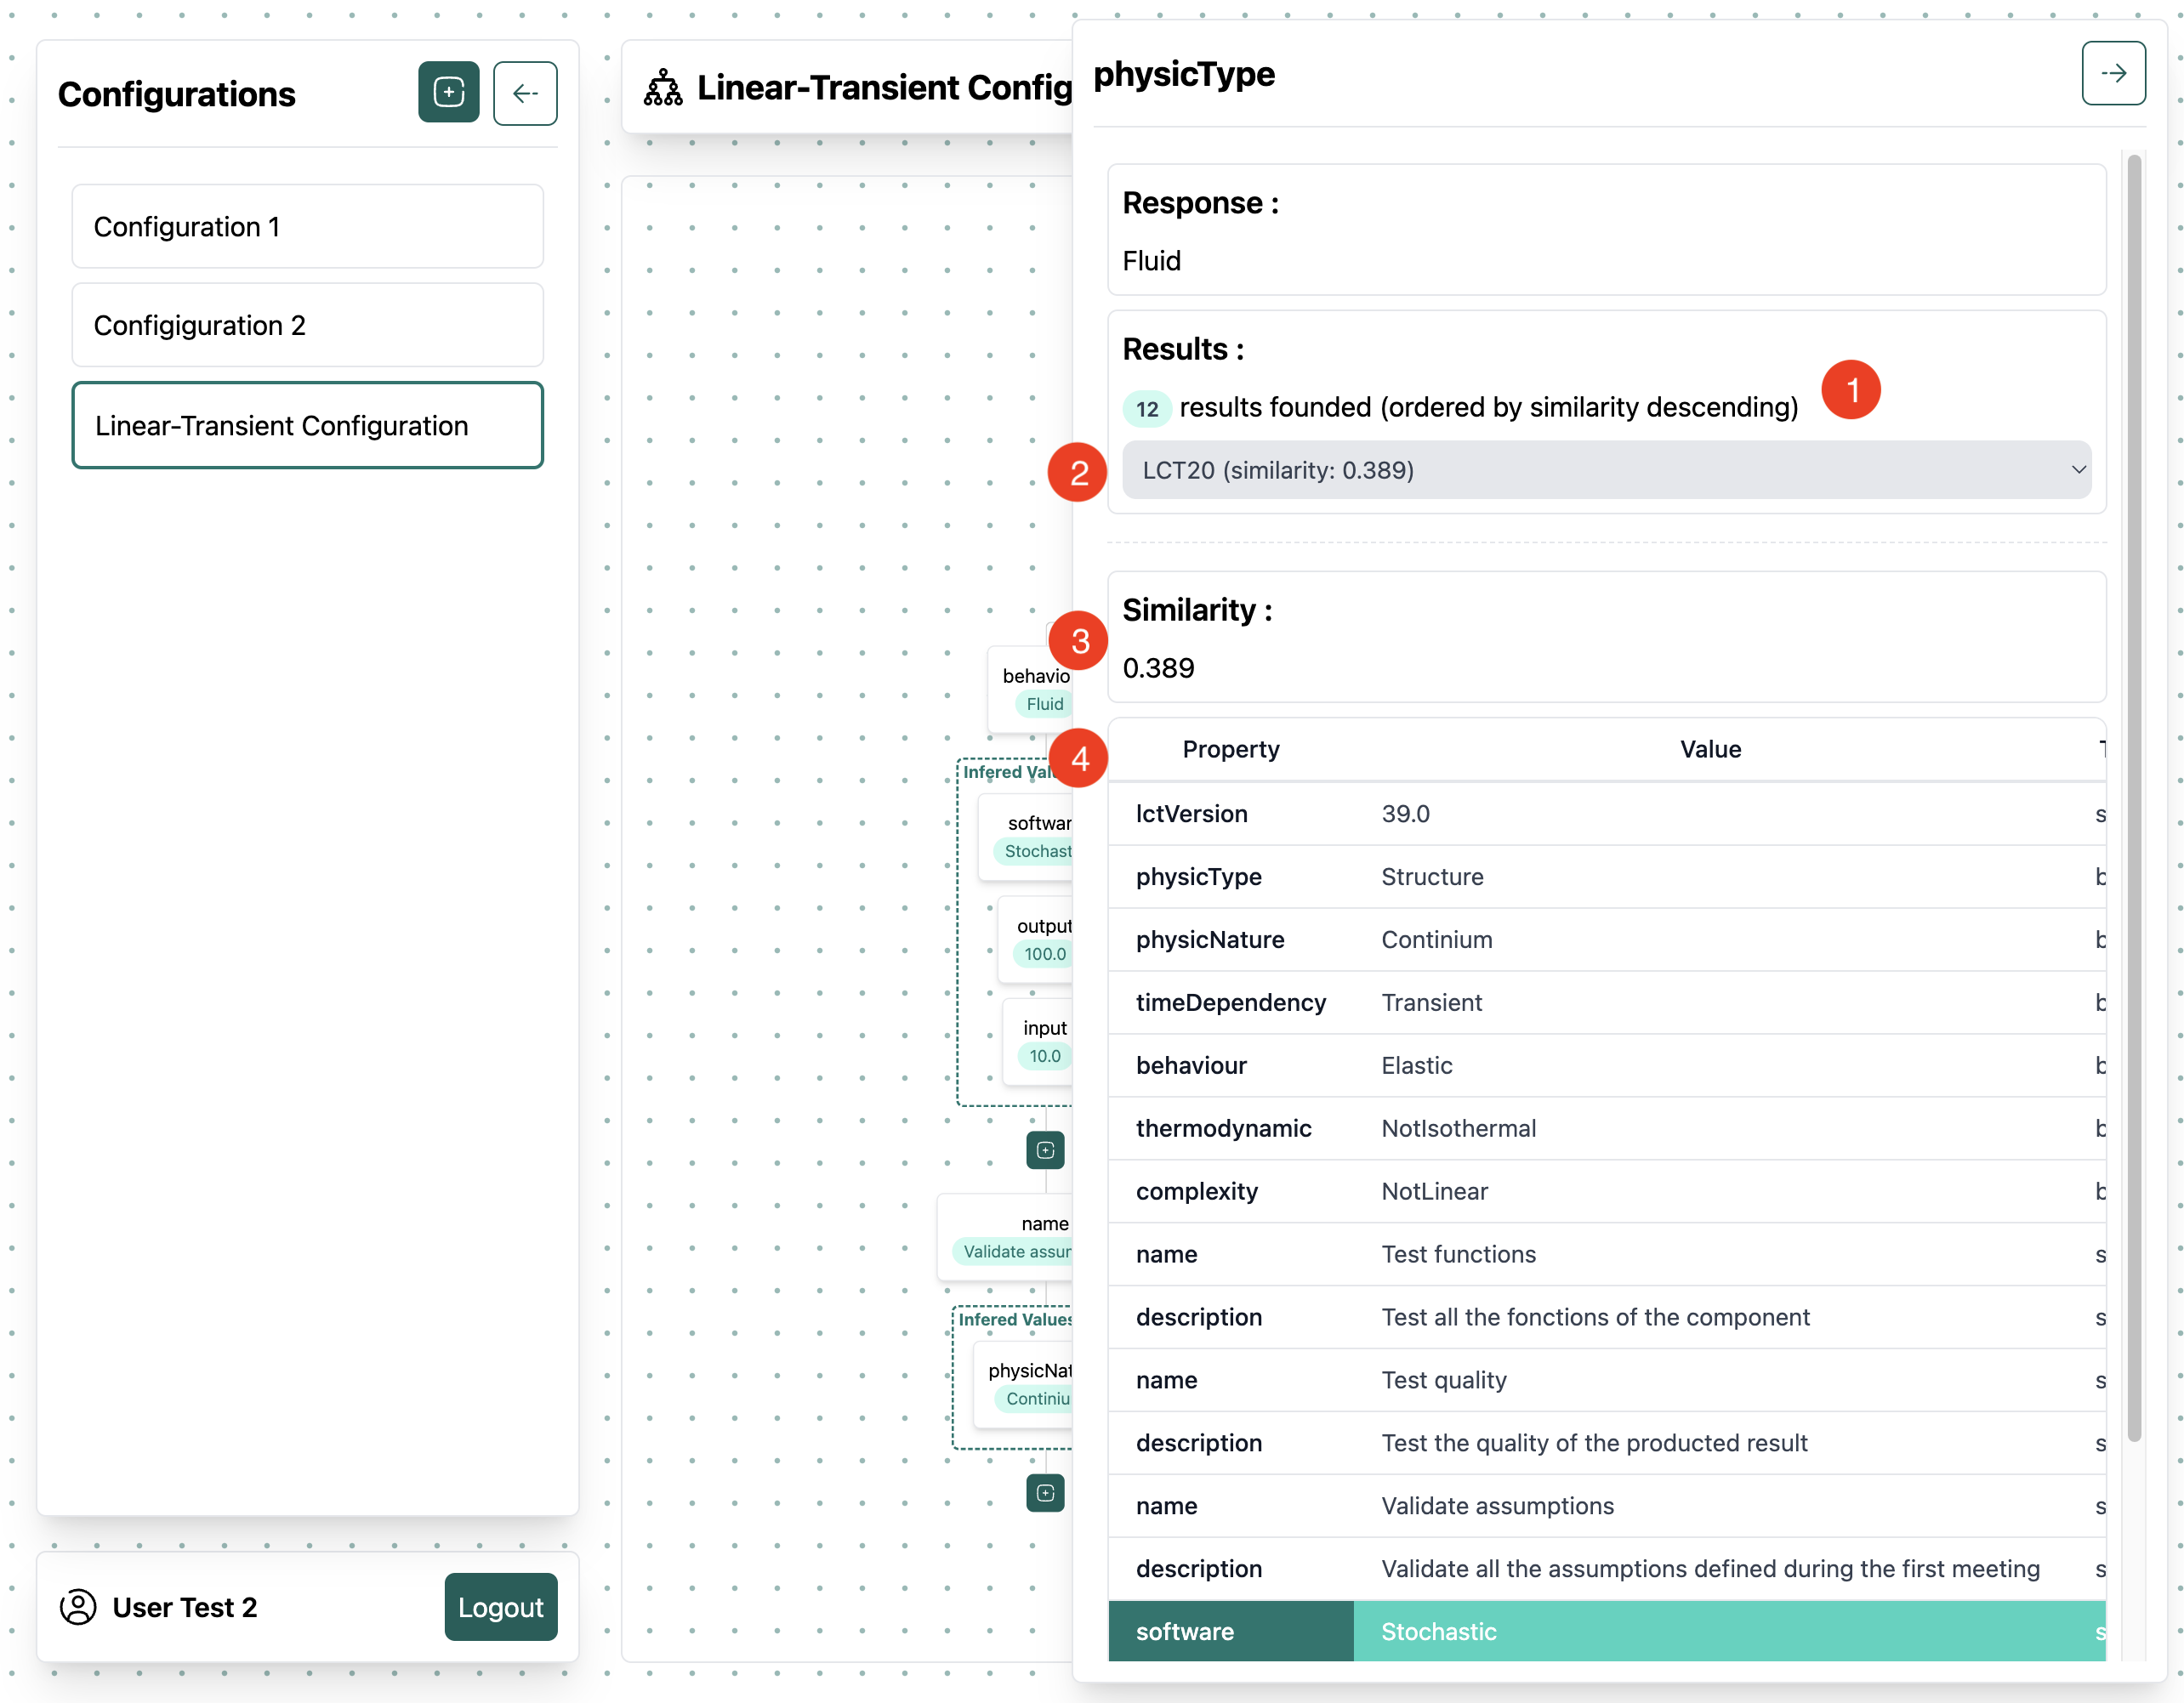
\includegraphics[width=\textwidth]{images/proto-demo-detail.png}}
    \caption{\label{fig:proto-demo-detail}  Inspect the details of a node}
    \end{figure}




    
\clearpage
%\section{Evaluation\label{sec:evaluation}}
In this chapter, we present a comprehensive evaluation of the solution developed to support configuration processes. The evaluation aims to determine the effectiveness, accuracy, ease of use, and overall performance of the platform, based on feedback from potential users.\\



\subsection{Methodology}
We used a multi-faceted approach to evaluate the platform, combining quantitative and qualitative methods. The main source of data was a Google form survey distributed to a variety of potential users, ranging from novices to automotive industry professionals performing simulation configuration tasks. The survey comprises twenty-one questions covering various aspects of platform functionality, user experience, and adoption potential.\\


% Is the result good? How efficient?
\subsection{Participant Demographics}
The survey gathered responses from a diverse group of automotive industry participants, including engineers, researchers, and managers. Respondents demonstrated a balanced spread of experience, with 35\% from 0 to 2 years, 30\% from 3 to 5 years, 20\% from 6 to 10 years, and 15\% with more than 10 years' experience. This diversity is crucial to understanding how easy it is to use the platform at different levels of expertise.\\


\subsection{Platform Usage and Frequency}
The results showed that a large proportion of participants (78\%) had previous experience of simulation configuration platforms, and that 65\% frequently performed simulation configuration tasks. This created a user base with a reasonable level of expertise in the field.\\


\subsection{User Interface and Experience}
Participants rated the platform's user interface with an average score of 4.2 out of 5, indicating a generally positive perception. In addition, 82\% of users found navigation on the platform intuitive, confirming its clarity and ease of use.\\


\subsection{Effectiveness and Accuracy}
The platform's effectiveness in identifying similar simulations based on key attributes received an average score of 4.4 out of 5. In addition, 88\% of respondents said that the platform's suggestions for parameter values were relevant to their simulation configuration needs. This suggests a promising capability for knowledge graph-based identification.\\
While the majority of users (88\%) felt that the suggested parameter values were relevant, 12\% expressed concerns about their accuracy. Further study of specific cases of inaccuracy will be essential to refine the system.\\


\subsection{Speed and Efficiency}
The platform proved its efficiency, achieving an average score of 4.3 out of 5 for the speed with which similar simulations were identified. A notable 90\% of the participants experienced no delays or performance issues during their interaction with the platform. However, 10\% of respondents reported occasional delays, requiring further investigation of potential performance bottlenecks.\\
Users generally agreed (85\%) that the platform efficiently completed tasks related to simulation setup. Any reported inefficiencies will be investigated to improve the overall workflow.\\


\subsection{Usability}
Ease of use was well received, with an average score of 4.5 out of 5. This indicates that the platform's features and functionality were clear and easy to understand for the majority of users.\\
Open-ended responses provided valuable insights into user expectations and specific areas for improvement, such as enhanced visualization tools and additional customization options.\\


\subsection{Suggestions for Improvement}
Participants provided valuable suggestions for improvement, particularly concerning visualization functions and the incorporation of additional domain-specific parameters. These ideas will guide future developments to meet user needs and preferences.\\


\subsection{Compatibility}
An encouraging 85\% of respondents confirmed that the platform would integrate seamlessly with their existing simulation tools or workflows. The remaining 15\% reported minor compatibility issues, which will be addressed in future updates.\\


\subsection{Likelihood to Adopt}
The likelihood of users adopting the platform for their simulation configuration needs was favorable, with an average score of 4.2 out of 5. Positive feedback emphasized the platform's potential to streamline configuration processes, as well as its accuracy and efficiency, as key factors influencing their decision.\\


The results of the evaluation confirm the success of the solution. The positive feedback and constructive suggestions received from users will form the basis for future iterations of the platform, which will focus on meeting specific user needs and further enhancing its capabilities. The platform shows promising potential for practical adoption in real-life scenarios in the field of automotive simulation.



%\clearpage
\section{Discussion \label{sec:discussion}}
This chapter looks in detail at the development process, the strengths, and weaknesses of the developed platform, and its potential for further development. We will analyze the successes encountered during development, the difficulties encountered, and the overall effectiveness of the proposed solution.  Next, we will explore the perceived advantages and limitations of the platform based on user feedback and the limitations identified based on testing and evaluation. Finally, we will discuss suggestions for possible improvements.\\



\subsection{Development Phase}
    \subsubsection*{Positive Aspects}
    During development, several aspects have proven to be beneficial. The use of semantic technologies offered a structured and flexible approach to representing knowledge about simulations. Numerous meetings were held with other participants in the EP4.0 project to agree on the structure and standardization of the artifacts and metadata to be taken into account. This led to the construction of the diagram presented in \textbf{Section \ref{subsec:sim-archi}}. So, the development of a complete and detailed ontology for automotive simulations was an iterative process. The definition of appropriate classes, properties, and relationships required continuous refinement based on feedback from domain experts.\\
    
    The use of ontologies facilitated the definition of clear relationships between entities and domain properties. In addition, the use of SPARQL to query the knowledge graph enabled efficient retrieval and reasoning about the encoded information.\\

    The development of a user-friendly \acrshort{ui} proved crucial to user adoption. The interface enabled users to easily enter simulation attributes and receive configuration suggestions, streamlining the configuration process.\\

    
    \subsubsection*{Problems Encountered}
    Several problems were encountered during development. Feeding the knowledge graph with complete and accurate data proved to be a major challenge. Unfortunately, until the end, it was impossible to obtain a significant amount of data to use as examples. The solution opted for here was to define a few random examples respecting the interdependence rules presented in \textbf{Appendix \ref{annex:phy-bas-struc}}. To make the integration of these examples independent, an import system from an Excel file has been developed (see \textbf{Appendix \ref{annex:screen-excel}}). This allows anyone to add elements to the knowledge graph without having to understand how the code works.\\

    The development of the similarity-matching algorithm turned out to be complex. It was essential to strike a balance between precision and recall. While a highly accurate algorithm might identify only near-identical configurations, a less accurate approach might suggest irrelevant simulations. Although the platform suggests plausible parameter values, it is difficult to achieve perfect precision.\\


\subsection{Advantages of the Developed Solution}
    \subsubsection*{Positive Points Identified}
    The developed solution has several positive points. The first of these is knowledge reuse. The program facilitates knowledge reuse by capturing, storing, and using data from past successful simulations. This enables valuable lessons learned from previous projects to be incorporated into new configurations.\\

    Another positive aspect is the reduction in configuration time. The program can streamline the configuration process by identifying similar simulations and suggesting parameter values. Suggesting similar configurations and parameter values can significantly reduce the time needed to configure new simulations.\\
    
    The program also improves consistency. By relying on a centralized knowledge base, it promotes consistent configuration practices across different teams and projects. This reduces the risk of errors and inconsistencies in simulation configurations. Users can benefit from established best practices reflected in the data, facilitating knowledge transfer from experienced engineers to new users.\\

    
    \subsubsection*{Positive Feedback from other Participants and Potential Users}
    Once a stable version of the program had been obtained, it was presented to other project participants and potential users. They were very satisfied with the platform's user interface. What's more, they found navigation on the platform intuitive, confirming its clarity and ease of use. The platform's efficiency and speed in identifying similar simulations based on key attributes were also deemed effective. The majority of people reported that the platform's suggestions for parameter values were relevant to their simulation configuration needs. This suggests a promising capability for knowledge graph-based identification. To sum up, users generally agreed that the platform effectively performed the tasks assigned to it. 


\subsection{Limits of the Solution}
    \subsubsection*{Identified Limits}
    Although the platform is showing promising results, several limitations remain:
    
    \begin{itemize}
        \item \textbf{Dependence on data quality}:  The accuracy and effectiveness of the platform are highly dependent on the quality and completeness of the data contained in the knowledge graph.  Inconsistent or inaccurate data can lead to misleading suggestions.

        \item \textbf{Limited scope}: The current prototype focuses on specific types of automotive simulations. Extending the platform to a wider range of simulation configurations may require further development and refinement of the ontology.

        \item \textbf{Explainability of suggestions}:  Although the platform suggests parameters, it may not currently explain the reasoning behind the suggestions. Implementing functions to explain the reasoning process can boost user confidence and understanding.
    \end{itemize}

    
    \subsubsection*{Suggested Improvements}
    Participants made several valuable suggestions for improvement. The most important and frequent were as follows: 
    
    \begin{itemize}
        \item While the majority of users felt that the suggested parameter values were relevant, some expressed concerns about their accuracy. Further study of specific cases of inaccuracy will be essential to fine-tune the system.
    
        \item Although a large proportion of participants did not experience any delays or performance problems during their interaction with the platform. However, a few of them did report occasional delays, necessitating a closer examination of potential performance bottlenecks.
    
        \item Open-ended responses during brainstorming sessions provided valuable insights into user expectations and specific areas for improvement, such as improved visualization tools and additional customization options.
    \end{itemize}

\subsection{Outlook}
This study successfully demonstrates the feasibility of using semantic technologies to support the configuration of automotive simulations. The platform developed offers promising advantages in terms of efficiency, knowledge reuse, and consistency. Future efforts will focus on resolving the identified limitations, including integration with existing systems, incorporation of machine learning, and continuous enrichment of the knowledge graph. Further research could extend the platform's capabilities to support advanced simulation tasks such as parameter optimization and uncertainty analysis. By continually evolving and improving, the program has the potential to have a significant impact on the way simulations are configured, leading to faster development cycles and more robust design decisions.
\clearpage
\section{Conclusion and Future Work\label{sec:conclusion}}

This chapter summarizes and examines the strategy presented in this thesis. Additionally, the chapter provides a view on future work.

\subsection{Conclusion}

In conclusion, this thesis has addressed a critical challenge in simulation engineering by exploring the feasibility of using semantic technologies to improve simulation configuration processes. Firstly, the fundamentals of simulation engineering and semantic technologies were clarified. This provided a better overview of the factors involved in the main problem. In order to gain an overview of the various studies carried out on the subject, an SMS was produced. This also enabled us to discover the principle of \acrshort{cbr} and how it can be used with ontologies. It was then a question of identifying the various tools applying \acrshort{cbr} and determining whether these could be directly used to solve the problem of this thesis. But due to a number of factors, such as the fact that these tools are aging, it was concluded that a customized framework would have to be implemented. Before moving on to implementation, the ontology architecture and prototype were defined. The next step was to select the tools needed for implementation, with open-source as the main criterion. Once the implementation was complete, an evaluation was carried out by testing the prototype with different users and receiving their feedback via a survey form. This provided valuable information on the efficiency, ease of use and compatibility of the platform with the automotive industry. The results show that integrating semantic technologies into simulation configuration processes is a promising approach to the challenges faced by both experienced and novice simulation engineers.\\

With regard to the research goals from Chapter \ref{sec:introduction} the following activities
were carried out:

\begin{itemize}
    \item Objective \hyperref[G1]{\textbf{G1}}:  
    
    has been achieved, as an ontology has been set up in Section \ref{subsec:ontologyDev}. It includes all the elements identified as important for the configuration of a simulation, and models well the relationships and interdependencies between them.
    
    
    \item Objective \hyperref[G2]{\textbf{G2}}:
    
    has also been achieved. In the conception chapter (Chapter \ref{sec:conception}), the theory behind the framework is explained. Then in Chapter \ref{sec:implementation} the framework is implemented in python. The latter can be used by external applications via its API.
    
    
    \item The final \hyperref[G3]{\textbf{G3}}: objective has also been achieved. In the implementation chapter (Chapter \ref{sec:implementation}) a UI prototype was developed. It was then tested in Chapter \ref{sec:evaluation} to see whether or not it was effective.
\end{itemize}
    
\clearpage



Most of the research questions found beginnings of answers at the end of the  \acrfull{sms}. The research questions introduced in Section \ref{sec:introduction} could be answered as follows:\\

\begin{itemize}
    \item \hyperref[Q1]{\textbf{Q1}}: What are the main challenges and limitations of current configuration processes for simulations in the automotive industry?
    \begin{quote}
        As answered in Section \ref{para:sms_analysis}, simulation configuration is mainly exposed to complexity concerns, a lack of standardization, the long time needed for configuration and limited durability.\\
    \end{quote}

    \item \hyperref[Q2]{\textbf{Q2}}: How can semantic technology be used to support simulation configuration processes?
    \begin{quote}
        Semantic technologies can be used to build ontologies. The advantage of ontologies is that they are machine-readable and enable more advanced semantic structuring of data. These ontologies can be used to structure the data needed to configure simulations, highlighting the relationships and interdependencies between the elements involved in the process.\\
    \end{quote}
    
    \item \hyperref[Q3]{\textbf{Q3}}: What are the requirements for a semantics-based configuration tool for simulations in the automotive industry?
    \begin{quote}
        As requirements we can have:
        \begin{itemize}
            \item \textbf{Semantic matching algorithm}: The tool must implement advanced semantic matching algorithms capable of comparing and identifying similarities between attributes in new simulations and data in the existing knowledge graph. This enables the tool to suggest relevant previous simulations as references.
            \item \textbf{Parameter value deduction}: The configuration tool must be able to deduce plausible values for the parameters of new simulations based on the similarities identified. This requires advanced reasoning capabilities to propose values that align with historical data.
            \item \textbf{User interface and interaction}: A user-friendly interface is essential to enable simulation engineers to interact easily with the tool. The interface must allow the input of key attributes for new simulations and provide clear suggestions for parameter values.
            \item \textbf{Accuracy and reliability}: The configuration tool should prioritize accuracy by suggesting relevant previous simulations and plausible parameter values. Reliable results are essential to guarantee the quality of configured simulations.\\
        \end{itemize}
    \end{quote}
    
    \item \hyperref[Q4]{\textbf{Q4}}: What existing semantic technologies and standards are applicable to the field of systems engineering and simulation configuration, and how can they be adapted to support simulation configuration processes?
    \begin{quote}
        In the field of systems engineering and simulation configuration, several existing semantic technologies and standards can be applied to improve processes. Adapting these technologies involves integrating them into a coherent framework tailored to the needs of simulation configuration. Here are a few relevant technologies and standards:
         \begin{itemize}
             \item RDF (Section \ref{subsubsec:rdf})
             \item OWL (Section \ref{para:owl})
             \item SPARQL (Section\ ref{para:sparql})
             \item Ontology Development Tools: as protégé (Section \ref{subsubsec:protege})
             \item Semantic Reasoning Engines: like Pellet or HermiT (Section \ref{para:logInf})
             \item Knowledge Graphs or ontologies (Section \ref{subsubsec:ontology})
         \end{itemize}
        
        Adapting these technologies involves designing a complete architecture that seamlessly integrates them into the simulation configuration workflow. This adaptation must take into account the specific needs and characteristics of the automotive industry.
    \end{quote}
\end{itemize}


 
\subsection{Future Work}
As presented throughout this thesis, the work was limited to setting up a prototype. But prototyping also means the possibility of further improvements. Here is a list of additional work that could be implemented in future projects:

\begin{itemize}
    \item \textbf{Scalability testing and optimization}: Carry out extensive scalability testing to ensure that the platform's performance remains optimal as the volume of data and complexity of simulation scenarios increase. Implement optimization techniques to efficiently handle larger knowledge graphs and data sets.
    
    \item \textbf{Benchmarking against industry standards}: Conduct benchmarking studies against industry standards to validate the platform's performance and compare it with existing solutions. This ensures that the semantic technology solution remains competitive and relevant in the rapidly evolving field of simulation configuration.
    
    \item \textbf{Enhanced Knowledge Graph}: Add more annotations to the relations present in the ontology. For example, there could be a description of each relationship, explaining the interdependence between the two Nodes (subject and predicate). These annotations will be used in the user interface to further support the user's choice of values.
    
    \item \textbf{Integration with simulation platforms}: Work towards seamless integration with the simulation platforms most widely used in the automotive industry. This could involve the development of plugins or connectors enabling direct interaction with commonly used simulation tools, facilitating a more streamlined and interconnected workflow.
    
    \item \textbf{User training and documentation}: Develop comprehensive user training documents and materials to facilitate the on-boarding process for new users. Provide tutorials, case studies and best practices to ensure that users can effectively exploit the full potential of the platform.
\end{itemize}


\clearpage

% Remove the following line if you want to have only the actually referenced references printed.
%\nocite{*}
\printbibliography[heading=bibintoc,title=References]
\clearpage

\appendix

\phantomsection
\section*{Appendices}
\addcontentsline{toc}{section}{Appendices}
\renewcommand{\thesubsection}{\Alph{subsection}}

\label{annex:framework}

\subsection{Statechart Inheritance in Rhapsody\label{annex:proto_inheritance}}

A concrete prototype that makes use of stepwise customisation was implemented in Rhapsody to
show how state machine inheritance can be used and to find possible limitations.




\clearpage
\subsection{State Machine Model Data Structure\label{annex:proto_delta}}

\begin{lstlisting}[language=CXX, label={lst:proto_sm_model}, caption={State machine model data structure.}]

enum StateType {
    Machine,
    Simple,
    Parallel,
    Composite,
    Initial,
    Final
};

struct State {
    string id;
    StateType type;
    State* parent;
    list<State*> children;
    string do_activity_id;
    string entry_action_id;
    string exit_action_id;
};

struct Transition {
    State* source;
    State* target;
    string event_id;
    string guard_id;
    string action_id;
};

struct StateMachine : State { // type = Machine;
    list<State*> m_all_states;
    list<Transition*> m_all_transitions;
};

\end{lstlisting}

Listing~[].


\clearpage
\subsection{State Machine Model Definitions\label{annex:impl_basic_sm}}

\begin{lstlisting}[language=CXX, label={lst:annex_basic_model}, caption={Basic life cycle without omissions.}]
struct ModelBuilder : IModelBuilder {

    std::unique_ptr<Model> MakeModel() override {
        auto model = std::make_unique<Model>("sm");

        // add states
        AddState(*model, Initial,   "Initial");
        AddState(*model, Composite, "On");
        AddState(*model, Final,     "Off");
        AddState(*model, Initial,   "On.Initial",
                                    "On");
        AddState(*model, Composite, "On.NotOperational",
                                    "On");
        AddState(*model, Simple,    "On.Operational",
                                    "On");
        AddState(*model, Initial,   "On.NotOperational.Initial",
                                    "On.NotOperational");
        AddState(*model, Simple,    "On.NotOperational.Starting",
                                    "On.NotOperational",
                                    "ActivityStarting",
                                    "ActionStartingEntry");
        AddState(*model, Simple,    "On.NotOperational.NotReady",
                                    "On.NotOperational");
        AddState(*model, Simple,    "On.NotOperational.Initialising",
                                    "On.NotOperational",
                                    "ActivityInitialising",
                                    "ActionInitialisingEntry");
        AddState(*model, Simple,    "On.NotOperational.Ready",
                                    "On.NotOperational");
        AddState(*model, Simple,    "On.NotOperational.Enabling",
                                    "On.NotOperational",
                                    "ActivityEnabling",
                                    "ActionEnablingEntry");
        AddState(*model, Simple,    "On.NotOperational.Disabling",
                                    "On.NotOperational",
                                    "ActivityDisabling",
                                    "ActionDisablingEntry");
        // add transitions
        AddTrans(*model, "Initial",
                         "On");
        AddTrans(*model, "On",
                         "Off",
                         "events.Exit",
                         "",
                         "ActionExit");
        AddTrans(*model, "On",
                         "",
                         "events.GetState",
                         "",
                         "ActionGetState");
        AddTrans(*model, "On",
                         "On",
                         "events.Reset");
        AddTrans(*model, "On.Initial",
                         "On.NotOperational");
        AddTrans(*model, "On.NotOperational.Initial",
                         "On.NotOperational.Starting");
        AddTrans(*model, "On.NotOperational.Starting",
                         "On.NotOperational.NotReady",
                         "events.Done",
                         "",
                         "ActionStartingDone");
        AddTrans(*model, "On.NotOperational.NotReady",
                         "On.NotOperational.Initialising",
                         "events.Init");
        AddTrans(*model, "On.NotOperational.Initialising",
                         "On.NotOperational.Ready",
                         "events.Done",
                         "",
                         "ActionInitialisingDone");
        AddTrans(*model, "On.NotOperational.Initialising",
                         "On.NotOperational.NotReady",
                         "events.Error",
                         "",
                         "ActionInitialisingFailed");
        AddTrans(*model, "On.NotOperational.Initialising",
                         "On.NotOperational.NotReady",
                         "events.Stop",
                         "",
                         "ActionInitialisingStopped");
        AddTrans(*model, "On.NotOperational.Initialising",
                         "On.NotOperational.Initialising",
                         "events.Init",
                         "",
                         "ActionInitialisingRestarted");
        AddTrans(*model, "On.NotOperational.Ready",
                         "On.NotOperational.Initialising",
                         "events.Init");
        AddTrans(*model, "On.NotOperational.Ready",
                         "On.NotOperational.Enabling",
                         "events.Enable");
        AddTrans(*model, "On.NotOperational.Enabling",
                         "On.Operational",
                         "events.Done",
                         "",
                         "ActionEnablingDone");
        AddTrans(*model, "On.NotOperational.Enabling",
                         "On.NotOperational.Ready",
                         "events.Error",
                         "",
                         "ActionEnablingFailed");
        AddTrans(*model, "On.Operational",
                         "On.NotOperational.Disabling",
                         "events.Disable");
        AddTrans(*model, "On.NotOperational.Disabling",
                         "On.NotOperational.Ready",
                         "events.Done",
                         "",
                         "ActionDisablingDone");
        AddTrans(*model, "On.NotOperational.Disabling",
                         "On.NotOperational.Ready",
                         "events.Error",
                         "",
                         "ActionDisablingFailed");

        return model;
    }
};
\end{lstlisting}





\end{document}
